%%
%% This is file `sigconf.tex',
%% generated with the docstrip utility.
%%
%% The original source files were:
%%
%% samples.dtx  (with options: `all,proceedings,sigconf')
%%
%% IMPORTANT NOTICE:
%%
%% For the copyright see the source file.
%%
%% Any modified versions of this file must be renamed
%% with new filenames distinct from sigconf.tex.
%%
%% For distribution of the original source see the terms
%% for copying and modification in the file samples.dtx.
%%
%% This generated file may be distributed as long as the
%% original source files, as listed above, are part of the
%% same distribution. (The sources need not necessarily be
%% in the same archive or directory.)
%%
%%
%% Commands for TeXCount
%TC:macro \cite [option:text,text]
%TC:macro \citep [option:text,text]
%TC:macro \citet [option:text,text]
%TC:envir table 0 1
%TC:envir table* 0 1
%TC:envir tabular [ignore] word
%TC:envir displaymath 0 word
%TC:envir math 0 word
%TC:envir comment 0 0
%%
%% The first command in your LaTeX source must be the \documentclass
%% command.
%%
%% For submission and review of your manuscript please change the
%% command to \documentclass[manuscript, screen, review]{acmart}.
%%
%% When submitting camera ready or to TAPS, please change the command
%% to \documentclass[sigconf]{acmart} or whichever template is required
%% for your publication.
%%
%%
\documentclass[sigconf]{acmart}
%%
%% \BibTeX command to typeset BibTeX logo in the docs
\AtBeginDocument{%
  \providecommand\BibTeX{{%
    Bib\TeX}}}

%% Rights management information.  This information is sent to you
%% when you complete the rights form.  These commands have SAMPLE
%% values in them; it is your responsibility as an author to replace
%% the commands and values with those provided to you when you
%% complete the rights form.
\setcopyright{acmlicensed}
\copyrightyear{2027}
\acmYear{2027}
\acmDOI{XXXXXXX.XXXXXXX}
%% These commands are for a PROCEEDINGS abstract or paper.
\acmConference[SIGMOD '27]{International Conference
on Management of Data}{June 13--19,
  2027}{Huntington Beach, CA}
%%
%%  Uncomment \acmBooktitle if the title of the proceedings is different
%%  from ``Proceedings of ...''!
%%
%%\acmBooktitle{Woodstock '18: ACM Symposium on Neural Gaze Detection,
%%  June 03--05, 2018, Woodstock, NY}
\acmISBN{978-1-4503-XXXX-X/2027/06}


\usepackage{subcaption}


% add usepackage by yma391
\usepackage[table]{xcolor}
\definecolor{singleviewbg}{RGB}{255,243,224}   % light orange
\definecolor{multiviewbg}{RGB}{227,242,253}    % light blue
\definecolor{ynote}{RGB}{142,36,170}
\newcommand{\ynote}[1]{\textcolor{ynote}{#1}}  % zhuoxing's comments

\usepackage{tikz}
\usepackage{pgfplots}
\pgfplotsset{compat=1.18,
  tpchaxis/.style={
    width=\columnwidth,
    axis line style={black!60},
    xtick pos=bottom, ytick pos=left,
    tick align=outside, tick style={black!60},
    ymajorgrids, grid style={black!12, very thin},
    tick label style={font=\scriptsize},
    label style={font=\small},
  }}
\definecolor{tpchS}{RGB}{31,90,166}
\definecolor{tpchQ}{RGB}{204,85,0}
\definecolor{tpchT}{RGB}{16,133,120}
\definecolor{tpchR}{RGB}{176,32,66}
\usepackage{enumitem}
% Query Schema
\usepackage{booktabs}
% \usepackage{amssymb}
\usepackage{graphicx}
\newcommand{\rot}[1]{\rotatebox{90}{\textbf{#1}}}
\newcommand{\usemark}{\scalebox{1.25}{$\bullet$}}









\begin{document}


\title{Entity/Re\-lation\-ship Modelling for (De-)Normalization}



%%
%% The "author" command and its associated commands are used to define
%% the authors and their affiliations.
%% Of note is the shared affiliation of the first two authors, and the
%% "authornote" and "authornotemark" commands
%% used to denote shared contribution to the research.





%\begin{comment}
\author{Author names suppressed due to double-blind reviewing}
%\end{comment}


\begin{comment}
\author{Zihui Yang}
\orcid{}
\email{zyan423@aucklanduni.ac.nz}
\affiliation{%
  \institution{University of Auckland}
  \city{Auckland}
  \country{New Zealand}
}


\author{Yuqian Ma}
\orcid{}
\email{yma391@aucklanduni.ac.nz}
\affiliation{%
  \institution{University of Auckland}
  \city{Auckland}
  \country{New Zealand}
}

\author{Zhuoxing Zhang}
\orcid{}
\email{zhuoxing.zhang@auckland.ac.nz}
\affiliation{%
  \institution{University of Auckland}
  \city{Auckland}
  \country{New Zealand}
}

\author{Philipp Skavantzos}
\orcid{}
\email{philipp.skavantzos@auckland.ac.nz}
\affiliation{%
  \institution{University of Auckland}
  \city{Auckland}
  \country{New Zealand}
}

\author{Sebastian Link}
\correspondingauthor
%\authornotemark[1]
\orcid{0000-0002-1816-2863}
\email{s.link@auckland.ac.nz}
\affiliation{%
  \institution{University of Auckland}
  \city{Auckland}
  \country{New Zealand}
}
\end{comment}




% \renewcommand{\shortauthors}{Trovato et al.}


\begin{abstract}
Normalization reduces the degree of data redundancy and update inefficiency that instances of a database schema can exhibit. Denormalization undoes some of these effects for the purpose of evaluating frequent queries faster. We establish an algebraic framework for denormalization using Entity/Relationship (E/R) modelling. Different from any previous work, our framework provides a conceptual understanding for the degree of data redundancy that E/R diagrams entail, which is independent from any logical and physical data models derived subsequently. Intuitively, links of an E/R diagram remove data redundancy while joining object types they link re-introduces data redundancy. For a given E/R diagram, generating denormalized E/R diagrams by joining object types via their links is shown to form a Boolean algebra. Its operations of meet, join, and negation are associated with the selection of views for a given workload of join queries. We conduct extensive experiments on our running example to illustrate our framework at an operational level. In addition, extensive experiments on TPC-H highlight how the framework performs on a well-known benchmark. This illustrates what conceptual insights can be derived from our framework and how they need to be complemented by practical considerations when moving to an operational workload.
\end{abstract}


\begin{CCSXML}
<ccs2012>

    <concept>
        <concept_id>10002951.10002952.10002953.10002959</concept_id>
        <concept_desc>Information systems~Entity relationship models</concept_desc>
        <concept_significance>500</concept_significance>
    </concept>
    <concept>
        <concept_id>10002951.10002952.10003190.10003205</concept_id>
        <concept_desc>Information systems~Database views</concept_desc>
        <concept_significance>500</concept_significance>
    </concept>
    <concept>
        <concept_id>10002951.10002952.10003212.10003214</concept_id>
        <concept_desc>Information systems~Database performance evaluation</concept_desc>
        <concept_significance>500</concept_significance>
    </concept>

</ccs2012>
\end{CCSXML}

\ccsdesc[500]{Information systems~Entity relationship models}
\ccsdesc[500]{Information systems~Database views}
\ccsdesc[500]{Information systems~Database performance evaluation}

\received{xx July 2026}
\received[revised]{xx xx 2026}
\received[accepted]{xx xx 2026}

%%
%% This command processes the author and affiliation and title
%% information and builds the first part of the formatted document.
\maketitle


\section{Introduction}

Database design aims at organizing the information of an application domain into units that help processing the anticipated workload of update and query operations as efficiently as possible. On one hand, Entity/Relationship (E/R) modelling and database normalization constitute methodologies resulting in database designs with quality guarantees. The latter refer to the elimination of data redundancy, which ensure a minimal overhead for integrity maintenance during updates. Apart from efficiency concerns, these methodologies are also perceived as producing database designs that represent the application domain coherently and logically in the digital world. We introduce our running example on which concepts and findings will be illustrated throughout our paper.

\begin{figure}
\includegraphics[width=.75\columnwidth]{figures/main/ER-model.png}
\caption{Normalized E/R Diagram $\textsc{D}$\label{fig:running-normalized}}
\end{figure}

\begin{example} We consider a simple \textsc{Sports} application. Games between home and away teams record their dates and the teams' scores. Statistics are recorded for players of a game, here the points they score. Teams have a coach, location and unique name. Players have a date of birth, height, weight and unique name. A game can be identified by its date and home team (other keys such as the data and away team may also hold), and the statistics is determined by the player and game. Figure~\ref{fig:running-normalized} shows the E/R diagram $\textsc{D}$ for this application. Entity types are represented by a rectangle with their name inside and attributes attached. Attributes that form the key are underlined. Relationship types are represented by diamonds with their name inside, attributes attached and links to each of their components with a potential role label attached to the link. Components that belong to the key have a dot on their link. The semantics can be taken from its relational database schema $\textsc{D}_r$ in which attributes are abbreviated:
\begin{itemize}\small
\item \textsc{Player}=\{P.n,P.d,P.h,P.w\} with key \{P.n\},
\item \textsc{Team}=\{T.n,T.c,T.l\} with key \{T.n\},
\item \textsc{Game}=\{G.h:T.n,G.a:T.n,G.d,G.hs,G.as\} with key \{G.d,G.h:T.n\} and foreign keys {[}G.h:T.n{]}$\subseteq$\textsc{Team}{[}T.n{]} and {[}G.a:T.n{]}$\subseteq$\textsc{Team}{[}T.n{]}
\item \textsc{Stats}=\{S.p,S.P.n,S.G.d,S.G.h:T.n\} with key \{S.P.n,S.G.d,S.G.h:T.n\}, foreign keys {[}S.P.n{]}$\subseteq$\textsc{Player}{[}P.n{]} and {[}S.G.d,S.G.h:T.n{]}$\subseteq$\textsc{Game}{[}G.d, G.h:T.n{]}
\end{itemize}
The E/R diagram $\textsc{D}$ is normalized as all functional and inclusion dependencies are represented by keys and foreign keys, respectively.
\end{example}

On the other hand, queries may require expensive join operations that are not supported well by the database designs. In fact, they are reliant on presenting some of the data redundantly. At design time, the target workload is often unknown or still unstable. Best practice uses methodologies for normalizing designs, and then applies some denormalization strategies when more information is available. Such strategies may introduce views, temporary or materialized, which aim at processing frequent and otherwise expensive queries more efficiently. Materialized views can lead to significant speed ups but also incur high maintenance costs as updates to base tables require recomputations of the views.

Despite the centrality of database design in database research and practice, there is only little work on denormalization. This is due to the challenges that this topic presents: denormalization is highly dependent on the workload, on the application domain, and the database system being used. Indeed, both application domain and workload may evolve with requirement changes, and different database systems provide different strategies to address those changes. Since denormalization occurs at operational level, it is challenging to offer insight at earlier stages of database design. Different to previous work, we aim at providing a principled methodology for denormalization at conceptual level, which can inform changes to initial designs in response to workload changes.

We start from the observation that data redundancy constitutes the primary principled measure to which degree a database design is (de-)normalized. E/R modelling aims at database design that is fully normalized. Surprisingly however, significant information that E/R diagrams represent has not been used by prior work to establish principles for denormalization. Indeed, every link of an E/R diagram does not only show the dependence of a higher-order object type from a lower-order object type, but removes the data redundancy that the lower-order object type would cause if it was part of the higher-order object type. When translated to a logical model, such as the relational model of data, each link is translated into a foreign key from the table of the higher-order object type to the table of the lower-order object type. Vice versa, foreign keys are primary tools for joining tables during query processing. In other words, joining these tables via a foreign key relationship undoes the effects of normalization, and should therefore be viewed as denormalization. In summary, the links of an E/R diagram constitute the primary principled mechanism for denormalization. This observations will lead us to discover an entire algebraic structure of E/R diagrams, representing different degrees of data redundancy and (de-)normalization. Since this framework occurs at the conceptual level, it will enjoy insight into denormalization that is indepepdent of any logical or physical constraints. We illustrate these ideas on our running example.

\begin{figure}
\includegraphics[width=.75\columnwidth]{figures/main/ER-model-folded.png}
\caption{E/R Diagram \textsc{D}' by joining $\textsc{Player}$ and $\textsc{Stats}$ in $\textsc{D}$\label{fig:running-folded}}
\end{figure}

\begin{example} The link from higher-order object type \textsc{Stats} to Entity type \textsc{Player} represents a foreign key in the corresponding relational database schema. Joining \textsc{Player} with \textsc{Stats} results in the E/R diagram $\textsc{D}'$ as in Figure~\ref{fig:running-folded}. Its corresponding relational database schema $\textsc{D}'_r$ is as follows:
\begin{itemize}\small
\item \textsc{Team}=\{T.n,T.c,T.l\} with key \{T.n\},
\item \textsc{Game}=\{G.h:T.n,G.a:T.n,G.d,G.hs,G.as\} with key \{G.d,G.h:T.n\}, foreign keys {[}G.h:T.n{]}$\subseteq$\textsc{Team}{[}T.n{]} and {[}G.a:T.n{]}$\subseteq$\textsc{Team}{[}T.n{]}
\item \textsc{Stats\_Player}=\{S.p,S.P.n,S.P.d,S.P.h,S.P.w,S.G.d,S.G.h:T.n\} with key \{S.P.n, S.G.d, S.G.h:T.n\}, functional dependency S.P.n$\rightarrow$ S.P.d, S.P.h, S.P.w and foreign key {[}S.G.d,S.G.h:T.n{]}$\subseteq$\textsc{Game}{[}G.d,G.h:T.n{]}
\end{itemize}
The new diagram contains one less entity type (table) and one less link (foreign key) but the key on \textsc{Player} has become a non-key functional dependency on the new object type \textsc{Stats\_Player}, which causes data redundancy: The information about the date of birth, height and weight needs to be repeated redundantly for every game the player participates in. The join operation has increased the degree of denormalization. Vice versa, extracting the \textsc{Player} from \textsc{Stats\_Player} would result in the E/R diagram $\textsc{D}$ in Figure~\ref{fig:running-normalized}, effectively increasing the degree of normalization. At the logical level, we may not want to replace the schema $\textsc{D}_r$ by $\textsc{D}'_r$, but rather supplement $\textsc{D}_r$ by the (materialized) view $\textsc{Player}\bowtie\textsc{Stats}$.
\end{example}

We will formalize these new insights and establish the classical E/R framework as a database design methodology that accommodates principled degrees of (de-)normalization as follows: %Our contributions can be summarized as follows.

(1) We establish E/R modelling as the first denormalization framework for the design of databases that enjoys logical and physical data independence. Every link of an E/R diagram controls the degree of (de-)normalization. Separating the lower-order object type, to which the link points, from the higher-order object type, from which the link points, eliminates data redundancy and increases the degree of normalization. Vice versa, joining the lower-order with higher-order object type via the link will cause data redundancy and increases the degree of denormalization.

(2) We show that progressive removal of links from a given E/R diagram by joining the linked object types results in a Boolean Algebra of (de-)normalized E/R diagrams. In fact, each of these diagrams corresponds to a database view that can operationalize the denormalization effort. The Boolean algebra does not only bring structure into the opportunities for denormalization, but also introduces the operations of meet, join, and negation on the E/R diagrams of the Boolean algebra. These operations will drive principled choices for view selection as the workload of the database evolves.

(3) We conduct extensive experiments on our running example and the TPC-H benchmark. These highlight the value of our framework for understanding the degree of (de-)normalization, because we illustrate various trade-offs between i) query and update performance, ii) temporary and materialized views, iii) single and multi-views; measuring, for example, when savings in query processing by views justify their maintenance.

(4) We extend our methodology to the case where more information about the query workload becomes available. As is the case in TPC-H, queries may benefit from joins that do not emerge from links in the E/R diagram. However, the queries can be regarded as further sources of information for our framework since we may add links between such object types to the given E/R diagram. This extends our (de-)normalization framework, which is purely schema-based, to a framework that is also informed by queries.

Classical E/R modelling offers a blueprint for designing database schemata that are fully normalized. We reposition E/R modelling more generally as a blueprint for designing database schemata that control the degree of (de)-normalization at the conceptual level.

Our article is organized as follows. We discuss related work in Sec.~\ref{sec:related}, review E/R modelling in Sec.~\ref{sec:er-model} before establishing our Boolean Algebra of Denormalized E/R Diagrams in Sec.~\ref{sec:boolean}. Experiments on our running example and the TPC-H benchmark are conducted in Sec.~\ref{sec:case-exp} and~\ref{sec:tpch-exp}, respectively, before concluding in Sec.~\ref{sec:conclusion}.

\section{Related Work}\label{sec:related}

Database normalization \cite{Armstrong_74_Dependency_Structures, Biskup_79_Synthesizing_Independent_DB_Schemas, Mannila_92_Relational_DB_Design, Batini_09_Encyclopedia_DBs, Abiteboul_95_Foundations_DBs} and denormalization \cite{Schkolnick_82_Effects_of_Denormalization, Sanders_01_Denormalization_Effects_RDBMS, Shin_06_Denormalization_Data_Warehouse, Lee_09_Side_Effects_Denormalization} are classical topics in database design. As noted in \cite{Shin_06_Denormalization_Data_Warehouse}, database denormalization has been a viable design practice, yet in the past, scholars have not put much focus on investigating the process. In contrast, there exists rich academic literature on database normalization. Moreover, in \cite{Shin_06_Denormalization_Data_Warehouse} the authors state that denormalization lacks a solid set of principles and guidelines. Nevertheless, the topic remains an active field of study \cite{Milicev_23_Hyper_Relations_Model_For_Denormalization, Fotache_25_Effects_of_DB_Normalization}. Denormalization is typically implemented through views that improve query performance while preserving a normalized underlying schema. Related research has extended these concepts from relational  \cite{Codd_70_Relational} to other databases\cite{Levene_99_DB_Design_Incomplete_Relations, Grahne_91_Incomplete_Information_in_Relational_DBs,Koehler_16_SQL_Schema_Design,Sanders_01_Denormalization_Effects_RDBMS,Link_19_DB_Design_Uncertain_Data,Tari_1997_Object_Normal_Form, Kemper_94_Materialization_in_Obect_Bases,Arenas_05_Normal_Forms_For_XML, Haw_11_Data_Storage_Query_Processing_XML, Skavantzos_25_3NF_BCNF_Graph, Han_25_Views_for_PGs, Pang_24_MV_Selection_And_MV_Based_Query_Planing_For_RPQs}.

Recent work has revisited denormalization from several perspectives. In \cite{Fotache_25_Effects_of_DB_Normalization}, lower logical normal forms are considered as higher denormalization strategies. Other work formulates denormalization as a cost-benefit optimization problem balancing OLTP redundancy against OLAP performance \cite{Kojic_20_Equilibrium_of_Redundancy}. In \cite{Milicev_23_Hyper_Relations_Model_For_Denormalization}, a hyper-relations model guides the selection of materialized views. Finally, denormalization has long been studied for star and snowflake schemas \cite{Inmon_05_Building_Data_Warehouse}. Warehouse-specific denormalization including partitioning, redundant and derived attributes using system-independent cost metrics \cite{Elmasri_15_Fundamentals_DB} have been investigated in \cite{Shin_06_Denormalization_Data_Warehouse}. In contrast, our work establishes a Boolean algebra of denormalization strategies directly from the E/R model at the conceptual level, identifying E/R links as primary mechanism for promoting/eliminating data redundancy.

Traditionally, the E/R model \cite{Chen_76_ER_Model, DBLP:books/daglib/0001129} underpins conceptual database design, providing a basis from which normalized schemata are derived. Denormalization is traditionally treated as subsequent optimization at the physical level~\cite{Batini_92_Conceptual_DB_Design}. More generally, database transformations have also been investigated at the conceptual level \cite{Ling_94_A_Normal_Form_OO_ER_Diagram, Ling_96_View_Update_In_ER_Approach, Rauh_95_Transformations_for_Normalization_of_ER_Schema, Hainaut_91_Entity_Generating_Schema_Transformations_for_ER_Model, Fahrner_95_Survey_DB_ERM_Based_Transformation}. In particular, \cite{Ling_96_View_Update_In_ER_Approach} developed a formal approach to update conceptual views. Collectively, previous work have establish methods for improving the quality of conceptual designs and supporting schema evolution. However, we are unaware of any framework for denormalization at the conceptual level.

Denormalization is commonly achieved by introducing controlled redundancy, using merged relations, replicated attributes or materialized views. Selecting performant views while balancing maintenance cost is a central challenge \cite{Gupta_95_Maintenance_Materialized_Views}. Consequently, this problem has been studied extensively \cite {Mami_11_View_Selection_Constraint_Satisfaction, Zhang_01_Evolutionary_Approach_View_Selection_DW, Zhang_99_Genetic_Algorithm_View_Selection_DW, Gupta_99_View_Selection_Maintenance_Cost_Constraint, Agrawal_00_Automated_View_Selection_and_Indexes_SQL, Mistry_01_View_Selection_Multi_Query_Optimization,Srinivasarao_22_Multi-Objective_MV_Selection_Flamingo_Search_Algorithm, Kechar_22_ZigZag_Plus_Global_Optimization_Algorithm_For_View_Selection}. Interested readers may consult some survey, such as \cite{Mami_12_Survey_of_View_Selection} for static and dynamic workloads. Our framework does not aim to improve view selection techniques at logical or physical level, but to provide a conceptual understanding which principled choices are available based on the degrees of data redundancy exhibited by E/R links.

\section{Entity/Relationship Modelling}\label{sec:er-model}

We summarize the syntax and semantics of E/R models~\cite{DBLP:books/daglib/0001129}.

\textbf{Entity types, Entities and Entity Sets.} Entities form the atomic units of a data model, and entities of the same type are modelled by the same entity type, that is, entity types consist of a finite set of attributes (properties). In addition, any entity of any type needs to be uniquely identifiable by a subset of these attributes. Formally, an \emph{entity type} $E$ consists of a finite, non-empty set $\textit{attr}(E)$ of attributes and a non-empty subset $\textit{id}(E)\subseteq\textit{attr}(E)$, called the \emph{key} of $E$ and every element $A\in\textit{id}(E)$ is called a key attribute of $E$. Every attribute $A$ has a domain $\textit{dom}(A)$, which is a non-empty set of possible values we can assign to any entity on that attribute.

An \emph{entity} $e$ of of type $E$ assigns a value $e(A)\in\textit{dom}(A)$ to every attribute of $E$. That is, $e:\textit{attr}(E)\rightarrow\bigcup_{A\in\textit{attr}(E)}\textit{dom}(A)$ such that for all $A\in\textit{attr}(E)$, $e(A)\in\textit{dom}(A)$. The collection $\textit{ent}(E)$ of entities over entity type $E$ is the Cartesian product over the domains assigned to attributes of $E$. Formally, $\textit{ent}(E)=\prod_{A\in\textit{attr}(E)}\textit{dom}(A)$.

An \emph{entity set} of type $E$ is a finite set $\mathcal{I}(E)\subseteq\textit{ent}(E)$ where different entities have different values on some key attribute. That is, for all $e,e'\in\mathcal{I}(E)$ where $e\neq e'$ there is some $A\in\textit{id}(E)$ such that $e(A)\neq e'(A)$. Hence, values on key attributes identify entities uniquely. The E/R model of our example has two entity types:
\begin{itemize}
\item \textsc{Player}=(\{name, dob, height, weight\},\{name\})
\item \textsc{Team}=(\{name, coach, location\},\{name\}).
\end{itemize}

\textbf{Relationship types, Relationships, and Relationship Sets.} Relationships are (complex) aggregations between (less complex) relationships and entities. Based on problems illustrated in the introduction, no directed cycles can exist between object types.

For every positive integer $k$, a \emph{relationship type} $R$ \emph{of order} $k$ consists of (i) a finite set $\textit{comp}(R)$ of relationship types, called \emph{components} of $R$, such that if $k=0$, then $\textit{comp}(R)=\emptyset$, and  if $k>0$, then every $R'\in\textit{comp}(R)$ is of order smaller than $k$ and there is some $R'\in\textit{comp}(R)$ of order $k-1$; (ii) a finite set $\textit{attr}(R)$ of attributes such that every $A\in\textit{attr}(R)$ has a domain $\textit{dom}(A)$; and (iii) a non-empty subset $\textit{id}(R)\subseteq\textit{comp}(R)\cup\textit{attr}(R)$, called the \emph{key} of $R$ such that the components in $\textit{id}(R)\cap\textit{comp}(R)$ are called \emph{key components} and the attributes in $\textit{id}(R)\cap\textit{attr}(R)$ are called \emph{key attributes} of $R$.

Hence, entity types are relationship types of order $0$ which have a non-empty set of attributes but no component. Relationship types of order $k>0$ do not need to have any attribute but they will have some relationship type of order $k-1$ as a component.

If the order of relationship type $R$ is $0$, the relationships of $R$ are the entities of $R$, that is, $\textit{rel}(R):=\textit{ent}(R)$. Otherwise, the order $k>0$ of $R$ is a positive integer, and the set $\textit{rel}(R)$ comprises all relationships $r$ of order $k$ where every $R'\in\textit{comp}(R)$ is mapped to a relationship $r(R')\in\textit{rel}(R')$ of the order of $R'$; and every $A\in\textit{attr}(R)$ is mapped to a domain value $r(A)\in\textit{dom}(A)$. In summary, we may also write $\textit{rel}(R)=\prod_{R'\in\textit{comp}(R)}\textit{rel}(R')\times\prod_{A\in\textit{attr}(R)}\textit{dom}(A)$. Collections of relationships over a relationship type $R$ of order $k$ are well defined, as all components of $R$ have an order strictly less than $k$ and relationships of order $0$ are entities.

Relationship sets must satisfy the unique key property, that is, a \textit{relationship set} over relationship type $R$ is a finite set $\mathcal{I}(R)\subseteq\textit{rel}(R)$ such that for all $r,r'\in\mathcal{I}(R)$ such that $r\neq r'$, $r(\textit{id}(R))\not=r'(\textit{id}(R))$.

When roles of components need highlighting we permit role labels $l$ as in $l:R'\in\textit{comp}(R)$, such as a $\textit{home}:\textsc{Team}$ playing an $\textit{away}:\textsc{Team}$, with labels $\textit{home}$ and $\textit{away}$ that distinguish teams.

Key attributes motivate the use of a foreign key semantics, in which for relationships $r$ of order $k>0$, we only use $\textit{rel}(R):=\prod_{R'\in\textit{id}(R)\cap\textit{comp}(R)}\textit{rel}(R')\times\prod_{A\in\textit{attr}(R)}\textit{dom}(A)$ to define relationships and relationship sets of order $k$. Indeed, this semantics minimizes the redundant duplication of attributes from components. Similar to the use of \emph{object type} we use the term \emph{object} (\emph{object set}) as reference to relationship (\emph{relationship set}) or entities (\emph{entity set}) without specifying which.

For our example, we have the relationship type \textsc{Game} of order 1 with \textit{comp}(\textsc{Game})=\{home:\textsc{Team}, away:\textsc{Team}\}, \textit{attr}(\textsc{Game})=\{date, h\_score, a\_score\}, and \textit{id}(\textsc{Game})=\{home:\textsc{Team}, date\}; and relationship type \textsc{Statistics} of order 2 with \textit{comp}(\textsc{Statistics})=
\{\textsc{Game}, \textsc{Player}\}, \textit{attr}(\textsc{Statistics})=\{points\}, \textit{id}(\textsc{Statistics})=\{\textsc{Game}, \textsc{Player}\}.

\textbf{Functional Dependencies.} Interestingly, many popular E/R frameworks do not accommodate constraints other than keys and foreign keys, emphasizing the perception that E/R modelling results in normalized database schemata (where all constraints can be expressed by only keys and a directed acyclic set of foreign keys). Since we are interested in denormalization, we explicitly add the capability of specifying a set of constraints with each object type, in this case a set of functional dependencies (FDs): $\textit{fd}(O)$ where each FD is an expression $X\rightarrow Y$ in which $X$ and $Y$ form a subset of $\textit{comp}(O)\cup\textit{attr}(O)$ and the semantics is that every pair of objects with values matching on all the components and attributes of the left-hand side $X$ also have values matching on all the components and attributes of the right-hand side $Y$. For example, object type $\textsc{Stats\_Player}$ in diagram $\textsc{D}'$ in Figure~\ref{fig:running-folded} has the FD $\textsc{Player}.\textit{name}\rightarrow\textsc{Player}.\textit{dob}, \textsc{Player}.\textit{height}, \textsc{Player}.\textit{weight}$, which results from the key of \textsc{Player} after joining it with \textsc{Statistics}.

\textbf{E/R Schemata and E/R Instances.} Referential integrity is deeply embodied in E/R Schemata. An \emph{Entity/Relationship Schema} (E/R Schema) is a non-empty, finite set $\mathcal{S}$ of object types such that for all relationship types $R\in\mathcal{S}$, all (labelled) components  $R'(l:R')\in\textit{comp}(R)$ of $R$, are also part of the schema, that is,  $R'(l:R')\in\mathcal{S}$. Relationship types need all their components.

The set $\mathcal{S}$ of object types we previously defined for the \textsc{Sports} application form indeed an E/R Schema. For instance, for $\textsc{Statistics}\in\mathcal{S}$ and  $\textsc{Game}\in\textit{comp}(\textsc{Statistics})$ we do have  $\textsc{Game}\in\mathcal{S}$.

These ideas on the schema level transcend naturally to the instance level. An \emph{Entity/Relationship instance} (E/R instance) $\mathcal{I}$ over E/R Schema $\mathcal{S}$ assigns to each entity type $E\in\mathcal{S}$, an entity set $\mathcal{I}(E)$ and to each relationship type $R\in\mathcal{S}$, a relationship set $\mathcal{I}(R)$ such that for each relationship $r\in\mathcal{I}(R)$ and for each object type $O\in\textit{comp}(R)$, $r(O)$ is an object in $\mathcal{I}(O)$. Indeed, higher-order objects cannot exist without lower-order objects they depend on.

\begin{figure}[t]
	\begin{subfigure}[b]{.475\columnwidth}
		\centering\includegraphics[width=\columnwidth]{figures/main/ERD_TPC-H.png}
		\caption{Full E/R Diagram\label{erd:tpch-property}}
	\end{subfigure}
	\begin{subfigure}[b]{.475\columnwidth}
		\centering\includegraphics[width=.8\columnwidth]{figures/main/ERD_TPC-H-query.png}
		\caption{Simple with Query Joins (red)\label{erd:tpch-keys}}
	\end{subfigure}
	\caption{Full and Simple E/R Diagram of TPC-H\label{fig:TPC-H}}
\end{figure}

\textbf{E/R Diagrams} are intuitive visualizations that facilitate communication about the target database. We recall a standard definition of E/R diagrams~\cite{DBLP:books/daglib/0001129}. An \emph{E/R Diagram} of E/R Schema $\mathcal{S}$ is a directed acyclic graph $\mathcal{G}=(V_G,E_G)$ such that the set $V_G$ of vertices contains the object types from the schema, $V_G:=\mathcal{S}$, and the set $E_G$ of directed edges, called \emph{E/R links}, represents the component relationships between object types, $E_G:=\{(R,R')\mid R'\in\textit{comp}(R)\}\cup\{(R,R')\text{ with edge-label }l\mid l:R'\in\textit{comp}(R)\}$. In particular, the order of object type $O\in\mathcal{S}$ is the maximum length across all directed paths from vertex $O\in V_G$ to any leaf in $V_G$.

E/R diagrams are visualized as explained in the introduction. Fig.~\ref{fig:running-normalized} shows the E/R diagram for our \textsc{Sport} example. Fig.~\ref{fig:TPC-H} shows the full and simple E/R diagram (only key features) of the TPC-H schema. The red links are not part of the diagram and will be explained later. Orders of object types are represented by shades of gray, starting with white (order 0) up to the darkest gray (order 4).

\textbf{Other E/R concepts}, such as weak entity types, specializations, and cardinality constraints can be captured by the E/R model presented. We consider the example \textsc{Manage} in Fig.~\ref{example:manage} where every manager is an employee and employees have managers. Specializations are sub-classes, which can be represented as unary relationship types $R=(\{R'\},\textit{attr}(R),\{R'\})$ whose key only consists of the singleton component $\{R'\}$. In our example, every manager is an employee, and as employees are identified by their \textit{emp\_id}, so are managers. Likewise, \textsc{Manager} is an example of a \emph{weak entity type} whose objects cannot be identified without other object types. In our example, \textsc{Managers} can only be identified by their component \textsc{Employee}. Cardinality constraints stipulate conditions on the number of relationships in which relationships of lower order can participate. In our example, employees can have at most one manager, which we may declare by $\textit{card}(\textsc{Managed},\textit{is}:\textsc{Employee})\le 1$. However, this is equivalent to the E/R key \textit{id}(\textsc{Managed})=\{\textit{is}:\textsc{Employee}\}. As \textit{id}:\textsc{Manager} is not a key component of \textsc{Managed}, there is no upper bound on how many employees a manager can manage. If this number should be restricted, say to five, we may stipulate $\textit{card}(\textsc{Managed},\textit{by}:\textsc{Manager})\le 5$. For a detailed treatment of E/R concepts and constraints, we refer to a standard textbook~\cite{DBLP:books/daglib/0001129}.

\begin{figure}[t]
	\begin{subfigure}[b]{.45\columnwidth}
		\centering\includegraphics[width=.75\columnwidth]{figures/main/managed.png}
		\caption{E/R Diagram\label{erd:manage}}
	\end{subfigure}\hfill
	\begin{subfigure}[b]{.525\columnwidth}
		\centering\includegraphics[width=.75\columnwidth]{figures/main/managed-rdm.png}
		\caption{Matching Relational Schema\label{rdm:manage}}
	\end{subfigure}
	\caption{E/R Diagram and Its Matching Relational Database Schema  \textsc{Manage}\label{example:manage}}
\end{figure}


\section{A Boolean Algebra of E/R Diagrams}\label{sec:boolean}

Based on E/R links providing a principled measure of data redundancy, we surface a Boolean algebra of de-normalized E/R diagrams. This provides a fundamental understanding of the opportunities (de-)normalization may bring, already at the conceptual level.

\subsection{The Partially-ordered Set of Folds}

First, we ``fold'' a given E/R diagram by joining the object types connected by E/R links. In the true sense of the word, folding undoes effects of normalization and is therefore a principled approach towards denormalization at the conceptual level. Indeed, the number of folds we apply is proportional to the level of denormalization.

\begin{definition} Let $\mathcal{S}$ denote an E/R schema with object types $O$ and $O'$ such that $O'\in\textit{comp}(O)$, the \emph{fold} of $O'$ into $O$ is defined as the object type $O_f=(\textit{comp}(O_f),\textit{attr}(O_f),\textit{id}(O_f),\textit{fd}(O_f))$ consisting of:
\begin{itemize}
\item $\textit{comp}(O_f)=\textit{comp}(O)-\{O'\}\cup\bigcup_{C\in comp(O')}C$
\item $\textit{attr}(O_f)=\textit{attr}(O)\cup\bigcup_{A\in \textit{attr}(O')}O'.A$
\item $\textit{id}(O_f)=id(O)-\{O'\}\cup\bigcup_{A\in\textit{id}(O')}O'.A$
\item $\textit{fd}(O_f)=\textit{fd}_f(O)\cup\{\textit{id}(O')\rightarrow\textit{comp}(O')\cup\textit{attr}(O')\}\cup\textit{fd}(O')\}$ where $\textit{fd}_f(O)$ results from replacing every occurrence of $O'$ in every FD of $\textit{fd}(O)$ by $\textit{id}(O')$.
\end{itemize}
We define $\mathcal{S}_f=\mathcal{S}-\{O,O'\}\cup\{O_f\}$, if there is no $O''\in\mathcal{S}-\{O'\}$ such that $O'\in\textit{comp}(O'')$, and otherwise $\mathcal{S}_f=\mathcal{S}-\{O\}\cup\{O_f\}$. The E/R schema $\mathcal{S}_f$ is called the fold of $\mathcal{S}$ by $O'$ into $O$.
\end{definition}



In other words, in the fold $O_f$ of $O'$ into $O$, (i) the components of $O_f$ are all the components of $O$ except $O'$ and all the components of $O'$, (ii) the attributes of $O_f$ are all the attributes of $O$ and all the attributes of $O'$, (iii) the key of $O_f$ consists of all key components of $O$ other than $O'$ and all key components of $O'$, plus all key attributes of $O$ and all key attributes of $O'$, and (iv) the fds of $O_f$ consist of the fds of $O$ where occurrences of $O'$ have been replaced by the $\textit{id}(O')$, the fds of $O'$ and the fd $\textit{id}(O')\rightarrow O'$. It is the latter FD that introduces additional data redundancy into the fold, and therefore a higher degree of de-normalization.

\begin{figure}
\begin{subfigure}[t]{.475\columnwidth}
\includegraphics[width=\columnwidth]{figures/main/short-14.png}
\caption{Fold $\mathcal{S}^4_1$ of $\mathcal{S}_0$\label{fig:short-14}}
\end{subfigure}
\begin{subfigure}[t]{.475\columnwidth}
\includegraphics[width=\columnwidth]{figures/main/short-25.png}
\caption{Fold $\mathcal{S}^5_2$ of $\mathcal{S}^4_1$\label{fig:short-25}}
\end{subfigure}
\caption{Folds with different degrees of de-normalization\label{fig:folds}}
\end{figure}

\begin{example} The fold $\mathcal{S}_1^4$ of $\mathcal{S}_0$ by \textsc{Game} into \textsc{Stats} contains the new object type \textsc{Stats\_Game} (\textsc{SG}) with
\begin{itemize}\small
\item \textit{comp}(\textsc{SG})=\{\textsc{Player},home:\textsc{Team},away:\textsc{Team}\}
\item \textit{attr}(\textsc{SG})=\{points, date, h\_score, a\_score\}
\item \textit{id}(\textsc{SG})=\{home:\textsc{Team},\textsc{Player},date\}
\item \textit{fd}(\textsc{SG})=\{home:\textsc{Team}, date$\rightarrow$ away:\textsc{Team}, h\_score, a\_score\}.
\end{itemize}
$\mathcal{S}^4_1$ is illustrated in Figure~\ref{fig:short-14}.
\end{example}

Folds can be applied recursively as illustrated next.

\begin{example} The fold $\mathcal{S}^5_2$ of $\mathcal{S}^4_1$ by home:\textsc{Team} into \textsc{Stats\_Game} contains the following new object type \textsc{SG\_h:T} with
\begin{itemize}\small
\item \textit{comp}(\textsc{SG\_h:T})=\{\textsc{Player},away:\textsc{Team}\}
\item \textit{attr}(\textsc{SG\_h:T})=\{points, date, h\_score, a\_score, h:T.name, h:T.coach, h:T.location\}
\item \textit{id}(\textsc{SG\_h:T})=\{\textsc{Player},date,h:T.name\}
\item \textit{fd}(\textsc{SG\_h:T})=\{\{h:T.name, date\} $\rightarrow$ \{away:\textsc{Team}, h\_score, a\_score\}, h:T.name $\rightarrow$     \{h:T.coach, h:T.location\}\}
\end{itemize}
$\mathcal{S}^5_2$ is illustrated in Figure~\ref{fig:short-25}.
\end{example}

We now introduce a partial order between E/R schemata by defining when one schema is a fold for another.

\begin{definition}\label{def:fold}
E/R schema $\mathcal{S}'$ is a \emph{fold} for E/R schema $\mathcal{S}$ if either $\mathcal{S}'=\mathcal{S}$ or there is some sequence $\mathcal{S}=\mathcal{S}_1,\ldots,\mathcal{S}_{k+1}=\mathcal{S}'$ for some positive integer $k$ such that for all $j=1,\ldots,k$, $\mathcal{S}_{j+1}$ is the fold of $\mathcal{S}_j$ by $O'_{j}$ into $O_{j}$ for some object types $O'_{j},O_{j}\in\mathcal{S}_{j}$ such that $O'_{j}\in\textit{comp}(O_{j})$. We write $\mathcal{S}\le\mathcal{S}'$ iff $\mathcal{S}'$ is a fold for $\mathcal{S}$. Alternatively, we may call $\mathcal{S}$ an unfold for $\mathcal{S'}$ if and only if $\mathcal{S'}$ is a fold for $\mathcal{S}$.
\end{definition}

For example, Figure~\ref{fig:folds} shows that $\mathcal{S}^5_2$ is a fold for $\mathcal{S}_0$, due to $\mathcal{S}_0\le\mathcal{S}^4_1\le\mathcal{S}^5_2$. Next we define a poset of folds for an E/R schema.

\begin{definition}
Given E/R schema $\mathcal{S}$ with $d$ links, $\mathcal{F}(\mathcal{S})$ denotes the \emph{set of folds} for $\mathcal{S}$, and $(\mathcal{F}(\mathcal{S}),\le)$ as the partially-ordered set (poset) of folds for $\mathcal{S}$. Here, $\mathcal{S}$ is the bottom element and $\mathcal{S}_d$ is the top element of $\mathcal{F}(\mathcal{S})$, which is the unique fold for $\mathcal{S}$ with no links.
\end{definition}

\begin{figure*}
\includegraphics[width=\textwidth]{figures/main/BAD.png}
\caption{The Boolean algebra $(\mathcal{F}(\mathcal{S}_0),\le,\sqcup,\sqcap,\neg,\mathcal{S}_0,\mathcal{S}_4)$ with E/R schemata $\mathcal{S}^i_j$ of degree $j=0,\ldots,4$ and associated Join Views $V_l$ with their index number ($l$) for $l=0,\ldots,15$\label{fig:bad}}
\end{figure*}

Figure~\ref{fig:bad} shows the Hasse diagram of the poset for our example $\mathcal{S}_0$. Nodes are the E/R schemata $\mathcal{S}^i_j$ in which $i$ is the level of the lattice but also the degree of data redundancy for the schema. We use the E/R schema interchangeably with its associated E/R diagram. Each node shows its \emph{Join View} $V_l$ together with its index number $(l)$. These are defined as follows. Given a fold $\mathcal{S}'$ for $\mathcal{S}$, the \emph{Join View} $V_{\mathcal{S}'}$ of $\mathcal{S}'$ is the set of natural joins between schemata in the relational database schema for $\mathcal{S}$ necessary to obtain $\mathcal{S}'$.

For example, the fold $\mathcal{S}^4_2$ for $\mathcal{S}_0$ has Join View $V_8=\textsc{P}\bowtie \textsc{S}\bowtie\textsc{G}$. Note that $V_8$ joins $V_1$ and $V_4$ since they share relation schema $\textsc{S}$. The Join View $V_5$ associated with $\mathcal{S}^1_2$ consists of the materialized views $\textsc{P}\bowtie\textsc{S}$ and $\textsc{G}\bowtie h:\textsc{T}$, respectively. These do not share any relation schema, so are not joined further.

The poset $(\mathcal{F}(\mathcal{S}),\le)$ can be thought of as a structure of denormalized E/R schemata, but also as the structure of Join Views that generate this poset. Both interpretations are interchangeable. The first interpretation suggests the use of denormalized E/R schemata to boost query efficiency and keep update inefficiency manageable. While this is a possibility, best practice favours the use of the E/R schema $\mathcal{S}$ together with the Join View associated with the denormalized E/R schema. In this case, materialized views enjoy all benefits of an actual schema, including indices, such that optimizing the efficiency of query evaluation is maximised. Updates will be processed efficiently on the E/R schema, and the materialized views will typically need to be recomputed. The time for recomputing is then the cost of update maintenance.

Figure~\ref{fig:bad} illustrates on our running example how these two interpretation apply and can be used interchangeably. In what follows, we will develop our framework for the denormalized schemata, but it also applies directly to the interpretation as Join Views.

\subsection{Algebraic Foundations}

As illustrated by our running example $(\mathcal{F}(\mathcal{S}_0),\le)$, the poset exhibits a rich algebraic structure that we reveal now. This structure will provide conceptual insight how denormalization affects the execution of update and query workloads.

We start by introducing two binary and one unary operation on the poset $(\mathcal{F}(\mathcal{S}),\le)$. Firstly, we will define the \emph{join} of two elements as the least element that is the fold of both. We point out the double meaning of the word \textit{join}: It may refer to either a join operation from relational algebra, or a join operation in the algebraic structure of our poset as defined next. We do not want to change either of them since both are standard in their context.

\begin{definition}[join]\label{def:join}
Given two E/R schemata $\mathcal{S}_1$ and $\mathcal{S}_2$ in $\mathcal{F}(\mathcal{S})$, the join $\mathcal{S}_1\sqcup \mathcal{S}_2$ of $\mathcal{S}_1$ and $\mathcal{S}_2$ is the unique E/R schema $\mathcal{S}'$ in $\mathcal{F}(\mathcal{S})$ whose only links are those that occur in both $\mathcal{S}_1$ and $\mathcal{S}_2$.
\end{definition}

In our running example, the join of $\mathcal{S}^2_2$ and $\mathcal{S}^4_1$ is $\mathcal{S}^3_3$. Indeed, as the Hasse diagram in Figure~\ref{fig:bad} illustrates, the join is the least common node when tracing upward from the two given elements.

Secondly, we will define the \emph{meet} of two elements as the largest element that can be folded into each of them.

\begin{definition}[meet]\label{def:meet}
Given two E/R schemata $\mathcal{S}_1$ and $\mathcal{S}_2$ in $\mathcal{F}(\mathcal{S})$, the meet $\mathcal{S}_1\sqcap \mathcal{S}_2$ of $\mathcal{S}_1$ and $\mathcal{S}_2$ is the unique E/R schema $\mathcal{S}'$ in $\mathcal{F}(\mathcal{S})$ whose only links are those that occur in $\mathcal{S}_1$ or $\mathcal{S}_2$.
\end{definition}

In our running example, the meet of $\mathcal{S}^1_2$ and $\mathcal{S}^4_3$ is $\mathcal{S}^2_1$. In the Hasse diagram of Figure~\ref{fig:bad}, the meet is the greatest common node when tracing downward from the two given elements.

Finally, we will define the \emph{negation} of some element as the largest element whose meet is the bottom element $\mathcal{S}_0$, or equivalently, as the smallest element whose join is the top element $\mathcal{S}_d$.

\begin{definition}[negation]\label{def:negation}
Given an E/R schema $\mathcal{S}_1$ in $\mathcal{F}(\mathcal{S})$, the negation $\neg\mathcal{S}_1$ of $\mathcal{S}_1$ is the unique E/R schema $\mathcal{S}'$ in $\mathcal{F}(\mathcal{S})$ whose only links are those that are not links in $\mathcal{S}_1$.
\end{definition}

In our example, the negation of $\mathcal{S}^2_1$ is $\mathcal{S}^3_3$. Indeed, as the Hasse diagram in Figure~\ref{fig:bad} illustrates, the negation of $\mathcal{S}$ is the greatest element whose meet with $\mathcal{S}$ is the bottom element, or equivalently, the smallest element whose join with $\mathcal{S}$ is the top element.

Together, these operations define the structure of a \textit{Boolean algebra}, perhaps the most important algebraic structure in computer science. The most famous examples are the Boolean algebra of truth values with logical conjunction, disjunction, and negation, respectively; and the Powerset Algebra with set inclusion, union, intersection, and complement.

\begin{theorem}\label{thm:boolean} For every E/R Schema $\mathcal{S}$ with $d$ links,
\[\mathfrak{B}(\mathcal{S})=(\mathcal{F}(\mathcal{S}),\le,\sqcup,\sqcap,\neg,\mathcal{S},\mathcal{S}_d)\] is a Boolean Algebra with $2^d$ elements.
\end{theorem}

\begin{proof} Firstly, $(\mathcal{F}(\mathcal{S}),\le)$ is a poset since $\le$ enjoys the properties of reflexivity, anti-symmetry, and transitivity. These follow directly from Definition~\ref{def:fold}.

Following Definition~\ref{def:join}, the join of two elements is defined as the E/R schema whose set of links are those common to both elements. Hence, every link of the join is also a link of both elements, which means that the join is a fold of both elements. Since the join has no other link according to this definition, every other element which is a fold of both elements is also a fold of the join. In other words, the join is the least of all the elements that are folds for both. Hence, the join operation is well-defined.

Following Definition~\ref{def:meet}, the meet of two elements is defined as the E/R schema whose set of links are those occurring in at least one of the elements. Hence, every link of either element is also a link of the meet, meaning that both elements are a fold of the meet. Every other element for which both elements are folds must contain some link that is not a link in the meet. Hence, the meet is also a fold for each of those elements, making the meet the largest element for which both elements are a fold. Consequently, the meet operation is well-defined.

Following Definition~\ref{def:negation}, the negation of an element is defined as the E/R schema whose set of links are those links in $\mathcal{S}$ who are not links of the element. Since the given element and its negation have no links in common, their join must necessarily be the top fold $\mathcal{S}_d$. Every other element that has no links in common with the given element must contain some link that is not a link in the negation. Consequently, the negation is a fold for each of these other elements. Thus, the negation is the largest fold whose join with the given element is $\mathcal{S}_d$.

Finally, since $\mathcal{S}$ has $d$ links, there are $2^d$ subsets for the set of these $d$ links, each corresponding to a unique fold of $\mathcal{S}$.
\end{proof}

The result provides the first computational foundation to explore denormalized E/R schemata. In fact, the algebraic operations make it possible to reason about them. According to Stone's Representation Theorem~\cite{stone1936}, $(\mathcal{F}(\mathcal{S}),\le)$ with $d$ links is isomorphic to the Powerset Algebra generated by the set of $d$ links.

Apart from the underlying algebraic structure itself, the Boolean algebra provides plenty of conceptual insight into the design of databases. Links are the enablers of normalization in which redundancy is eliminated, while joins that are based on the links are enablers of denormalization in which redundancy is (re)introduced. In other words, the poset structures the degrees of (de)normalization. Likweise, the operations of join and meet provide conceptual strategies that identify which denormalized E/R schemata (or associated materialized Join Views, respectively) can address a given workload of join queries. These and more sophisticated strategies that are direct counterparts to more sophisticated algebraic properties of our Boolean algebra will be detailed next.

\subsection{Understanding View Selection Conceptually}\label{sec:conceptual-view-selection}

We explain how well-known concepts of partially-ordered sets and Boolean algebras offer conceptual insights into denormalization, in particular view selection. For this purpose, we utilize the interpretation by Join Views.

\subsubsection{Query Rewrites, Reduced Joins and Projections.} In general, given a join query $Q$ and a Join View $V$, we obtain the following rewrite in terms of $V$: $Q=(Q\sqcap\neg V)\sqcup (Q\sqcap V)$. In the special case where $V\le Q$, we have $Q=(Q\sqcap\neg V)\sqcup (Q\sqcap V)=(Q\sqcap\neg V)\sqcup V$, so $Q$ is the join of the view $V$ with the difference $Q-V=Q\sqcap\neg V$; and if $Q\le V$, then $Q$ is a projection of $V$.

For every given Join View $V\in\mathcal{F}(\emptyset)$, the primary filter $\lceil V\rceil$ consists of all the Join Views $V'$ where $V\le V'$, and the primary ideal $\lfloor V\rfloor$ consists of all the Join Views $V'$ such that $V'\le V$. Interestingly, \emph{every} query $Q$ in the filter $\lceil V\rceil$ benefits from materializing $V$ since $V$ reduces the join complexity of $Q$. Likewise, \emph{every} query $Q$ in the ideal $\lfloor V\rfloor$ benefits from materializing $V$ since $Q$ is a projection of $V$.

In our running example, $\lfloor V_{12}\rfloor=\{V_{12},V_5,V_8,V_9, V_1,V_2,V_4,V_0\}$, and $\lceil V_8\rceil=\{V_8,V_{12},V_{13},V_{15}\}$.

\subsubsection{Projections of Joins.} Given a workload $W$ as a collection of join queries, their join in the Boolean algebra is the smallest Join View $V$ that contains all join queries in $W$ in its principal ideal. Hence, all join queries in $W$ are projections of $V$. Since $V$ is the smallest Join View with this property, it offers the smallest projection effort and incurs the lowest maintenance costs in terms of a refresh. The higher the degree of $V$, the more queries are projections of $V$ but the higher the maintenance cost, too.

For our example, the join of $W=\{Q_5,Q_8\}$ is $V_{12}$, which has fewer projection costs and fewer maintenance costs than $V_{15}$.

\subsubsection{Reduced Joins of Meets.} Given $W$, their meet in the Boolean algebra is the largest Join View $V$ that contains all join queries in $W$ in its principal filter. Hence, all join queries $Q$ in $W$ become reduced joins $(Q-V)\sqcup V$ in terms of $V$. Since $V$ is the largest Join View with this property, it offers the biggest reduction in join complexity but also incurs the highest maintenance cost in terms of a refresh. The higher the degree of $V$, the bigger the join reduction but the higher the maintenance cost, too.

For our running example, given $W=\{Q_5,Q_8\}$ the meet is $V_1$, offering better join support but higher maintenance costs than $V_{0}$.

\subsubsection{Views of Ultra filters and Maximal ideals.} It is a natural question to ask whether there is a small set of materialized views that can support many join queries. Interestingly, the theory of Boolean algebras can provide some insight here.

The minimal elements that are different from the bottom element of a Boolean algebra are known as \emph{atoms}, and the maximal elements that are different from the top element are known as \emph{co-atoms}. Now interestingly, the filter of any atom $V$, also known as an \emph{ultra filter}, and the ideal of its corresponding co-atom $\neg V$, also known as a \emph{maximal ideal}, partition the elements of the Boolean algebra. That is, $\lceil V\rceil$ and $\lfloor \neg V\rfloor$ are disjoint, and their union is set of all elements.

This means for our Boolean algebra that every join query can be written as \emph{either} a projection of the co-atom \emph{or} as a reduced join with the atom. In other words, every join query benefits from the two materialized Join Views $V$ and $\neg V$, either as projections of $\neg V$ or reduced joins with $V$. In a finite Boolean algebra, there are no other elements with this property.

For our example, the atoms are $V_1,\ldots,V_4$ and the co-atoms are $V_{11},\ldots,V_{14}$. We have $\lceil V_1\rceil=\{V_1, V_5, V_6, V_8, V_{11}, V_{12}, V_{13}, V_{15}\}$ and $\lfloor \neg V_1\rfloor=\lfloor V_{14}\rfloor=\{V_{14},V_7,V_9,V_{10},V_2,V_3,V_4,V_0\}$.

%This is the homomorphism from the Boolean algebra to $\{0,1\}$ with the ideal of $\neg V$ being the kernel, and the filter of $V$ being the co-kernel. In a finite Boolean algebra, every ultrafilter is principal, so generated by an atom, and every homomorphism to $\{0,1\}$ is determined by an atom. In other words, we cannot have other materialized views such that all queries can be rewritten as either projections or simplified joins of the view and its complement.

\subsubsection{Disclaimer.} There are, of course, very practical concerns that need to be considered at later stages, in particular during logical and physical design. In fact, we do not claim that our framework can address view selection at the operational level better than any existing technique. Firstly, while joins constitute the most expensive database operations there are other operations that have a significant impact on the selection of views. Secondly, once a particular workload has emerged, the frequency of query and update operations matters significantly, and so does the size of the database. Thirdly, the specific data model and database system matter as well. However, these considerations only emerge once the database is operational, and are out-of-scope for work on a conceptual perspective of (de)normalization that enjoys logical and physical independence. Nevertheless, we do illustrate through our experiments how practical concerns can also be informed by our framework.

\begin{comment}
\section{Schema- and Query-Driven Denormalization}

Given a fully normalized E/R schema, denormalized schemas can be obtained by applying fold operations to its directed relationships. In the early stages of system design, analytical workloads are often not yet fully understood, and denormalization is therefore guided primarily by schema relationships. As business requirements and query workloads become available, additional workload-derived relationships can be incorporated to further customize the denormalization process. This leads to two complementary approaches: schema-driven and query-driven denormalization.

\subsection{Schema-driven Denormalization}

The following sections describe the generation of schema-driven configurations and the construction of their corresponding materialized structures.

\subsubsection{Schema-Driven Configurations}
Schema-driven denormalization uses the relationships defined in the database schema. In the relational model, these relationships correspond to primary-key and foreign-key relationships.

Each schema relationship may either be folded or left unchanged, giving rise to different denormalization configurations. A schema may generate many configurations. If a schema contains $n$ relationships, each of which may either be folded or left unchanged, the theoretical number of denormalization configurations is $2^n$. In the worst case, evaluating all configurations for a workload of $m$ queries requires considering up to $m \cdot 2^n$ query-configuration combinations. Therefore, identifying those that are effective for a given query is important. Let $Q_i$ denote an analytical query. A denormalization configuration is considered valid for $Q_i$ if it contains all information required by the query. Otherwise, the configuration is invalid. Among the valid configurations, some may contain additional information that is not required by $Q_i$, increasing both the size of the denormalized structure and the amount of data processed during query execution.


\subsubsection{Materialization Semantics}

When constructing schema-driven denormalization, the choice of join type is also important. Since denormalization should preserve all information represented in the schema, tuples should not be removed simply because they do not participate in a particular relationship. To preserve the information represented by the schema, relationships are materialized using left outer joins. Given two relations $R$ and $S$ connected through a primary-key/foreign-key relationship, where $S$ contains a foreign key referencing the primary key of $R$, the referenced relation is placed on the left-hand side of the join: $R \ \texttt{LEFT JOIN} \ S$. As additional relations are incorporated, the configuration is extended by applying left outer joins sequentially along the schema relationships.

\subsection{Query-driven Denormalization}


The following sections describe the generation of query-driven configurations and the construction of their corresponding materialized structures.


\subsubsection{Query-Driven Configurations}
Query-driven denormalization incorporates workload information when generating denormalized schemas. In addition to relationships defined by primary-key and foreign-key constraints, it considers workload-derived relationships identified from join predicates in analytical queries, where attributes from different relations are matched in the \texttt{WHERE} clause.

Query-driven denormalization expands the set of possible fold operations and therefore increases the number of candidate denormalization configurations. If a normalized schema contains $n$ schema-defined relationships and the workload introduces $k$ additional query-defined relationships, then the maximum number of possible configurations increases from $2^n$ to $2^{n+k}$. As a result, query-driven denormalization can explore denormalized schemas that are more closely aligned with the workload and may therefore provide greater performance benefits for specific analytical queries. In practice, it is not necessary to enumerate all possible configurations. Instead, configurations can be generated on a per-query basis. If a query references only a subset of relations, only denormalization configurations involving those relations need to be considered, substantially reducing the size of the search space.

\subsubsection{Materialization Semantics}

Unlike schema-driven, query-driven denormalization is guided by the requirements of the analytical workload. Since the objective is to support query execution rather than preserve all information represented in the schema, the choice of join type follows the semantics of the corresponding query. In most cases, workload-derived relationships are materialized using inner joins, since tuples that do not contribute to the query result can be excluded. The resulting materialized structures are often smaller than their schema-driven counterparts, reducing storage overhead and potentially improving query execution efficiency. Given two relations $R$ and $S$ connected through a query join condition, the materialized structure is constructed as $R \ \texttt{INNER JOIN} \ S$. When query semantics require unmatched tuples to be retained, left outer joins are used instead. As additional relations are incorporated, the configuration is extended by applying the join conditions specified by the query workload.
\end{comment}


\section{Experiments on Sports Database}\label{sec:case-exp}

Having established \emph{how} to denormalize a Boolean lattice of Join Views, we now ask \emph{which} denormalization to choose. For this purpose, we consider the fact-centric snowflake schema of our running example. Due to its small size, we can enumerate the \emph{entire} space of denormalizations as a lattice over its four join atoms. We can measure, at every node, the three quantities a designer trades off: storage redundancy, one-time build cost, and query time.

%The research questions fall into two classes, by how much of the workload they assume. The \emph{first is schema-driven}: which joins to materialize, decided from the schema before the query set is known. It has three parts: what drives redundancy (RQ1), how the fact-incident joins should be grouped into views (RQ2), and how dimension-side queries should be answered (RQ3). Sec.~\ref{sec:exp:analysis} answers these and distils each into a design principle. The \emph{second is workload-driven}: given a concrete query set, which single view to build (RQ4). Sec.~\ref{sec:exp:meetjoin} answers it through the lattice's \emph{meet} and \emph{join} (Sec.~\ref{sec:conceptual-view-selection}), which bracket the choice. Every effect we isolate is \emph{structural}, set by the schema and the workload rather than the data volume. The resulting guidance therefore carries beyond this schema to the industry-scale TPC-H study that follows.

\begin{table}[t]
  \centering
  \caption{Characteristics of database relations}
  \label{tab:sizes}
  \small
  \setlength{\tabcolsep}{6pt}
  \begin{tabular}{lccrr}
    \toprule
    Relation & Role & \#Attributes & $\textit{sf}{=}10$ & $\textit{sf}{=}100$ \\
    \midrule
    Player & dimension & 4 & 1,458 & 11,538 \\
    Team & dimension & 3 & 30 & 30 \\
    Game & dimension & 5 & 12,300 & 123,000 \\
    Stats & fact & 4 & 369,000 & 3,690,000 \\
    \midrule
    Total tuples & & --- & 382,788 & 3,824,568 \\
    Attribute values & & --- & 1,543,422 & 15,421,242 \\
    \bottomrule
  \end{tabular}
\end{table}
\raggedbottom


\subsection{Experimental Setup}\label{sec:exp:setup}

\paragraph{Schema and dataset.}
All experiments use the relational database $\mathrm{DB}_0$ for the E/R diagram of Fig.~\ref{fig:running-normalized} (primary keys underlined):
\begin{itemize}
  \setlength{\itemsep}{1pt}\setlength{\parsep}{0pt}\setlength{\topsep}{2pt}
  \item \textsf{Player}(\underline{name}, dob, height, weight);
  \item \textsf{Team}(\underline{name}, coach, location);
  \item \textsf{Game}(\underline{date, h\_name}, a\_name, h\_score, a\_score);
  \item \textsf{Stats}(\underline{date, h\_name, p\_name}, points).
\end{itemize}
\textsf{Stats} references \textsf{Player} and \textsf{Game}, and \textsf{Game} references \textsf{Team} twice (home and away) as shown in Fig.~\ref{fig:running-normalized}.
The many-to-one references make \textsf{Stats} the central \emph{fact} table: every tuple records one player's contribution to one game. \textsf{Player}, \textsf{Team}, and \textsf{Game} are \emph{dimension} tables that describe \textsf{Stats}, with \textsf{Game} an intermediate dimension that \textsf{Stats} references and that in turn references \textsf{Team}.
We generate instances at two \emph{scale factors} $\textit{sf}\!\in\!\{10,100\}$, where $\textit{sf}$ is the number of seasons: the number of teams is fixed at $30$, the number of games is $1230\cdot\textit{sf}$, $|\textsf{Stats}| = 30\cdot|\textsf{Game}|$, and players follow a rolling roster with $25\%$ inter-season turnover.
Table~\ref{tab:sizes} summarizes characteristics of the tables. \textsf{Stats} dominates the database by orders of magnitude.

\begin{comment}

\begin{figure*}[htbp]
\centering
\resizebox{0.9\textwidth}{!}{%
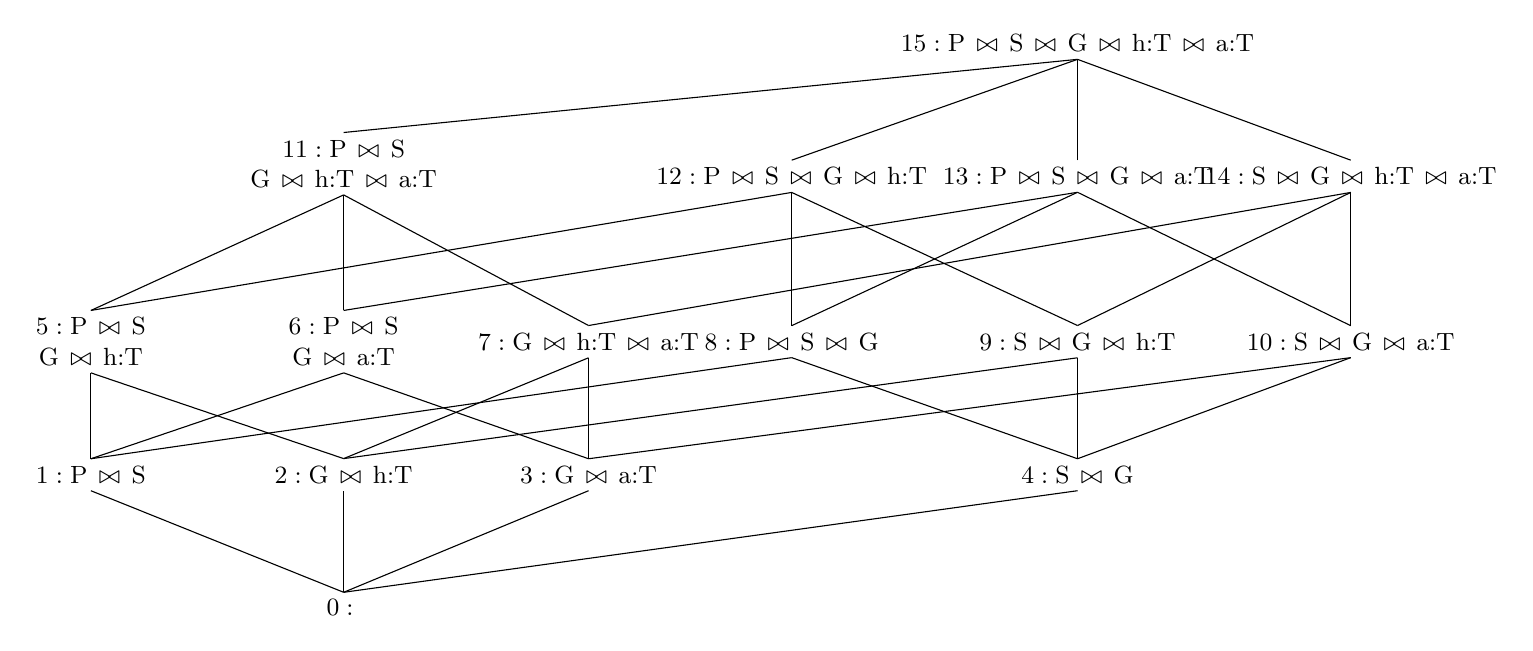
\begin{tikzpicture}[
  every node/.style={align=center, font=\small, inner xsep=3pt, inner ysep=2.5pt},
  edge/.style={draw=black, thin}
]
\newcommand{\J}{\,\bowtie\,}


%% Layer 0
\node (e)      at ( 3.68, 0.73) {$\mathrm{0:\; }\varnothing$};

%% Layer 1
\node (PS)     at ( 0.47, 2.42) {$\mathrm{1:\; }\mathrm{P}\J\mathrm{S}$};
\node (Gh)     at ( 3.68, 2.42) {$\mathrm{2:\; }\mathrm{G}\J \mathrm{h}{:}\mathrm{T}$};
\node (Ga)     at ( 6.79, 2.42) {$\mathrm{3:\; }\mathrm{G}\J \mathrm{a}{:}\mathrm{T}$};
\node (SG)     at (13.00, 2.42) {$\mathrm{4:\; }\mathrm{S}\J\mathrm{G}$};

%% Layer 2
\node (PSGh)   at ( 0.47, 4.11) {$\mathrm{5:\; }\mathrm{P}\J\mathrm{S}$\\$\mathrm{G}\J \mathrm{h}{:}\mathrm{T}$};
\node (PSGa)   at ( 3.68, 4.11) {$\mathrm{6:\; }\mathrm{P}\J\mathrm{S}$\\$\mathrm{G}\J \mathrm{a}{:}\mathrm{T}$};
\node (GhGa)   at ( 6.79, 4.11) {$\mathrm{7:\; }\mathrm{G}\J \mathrm{h}{:}\mathrm{T}\J \mathrm{a}{:}\mathrm{T}$};
\node (PSSG)   at ( 9.37, 4.11) {$\mathrm{8:\; }\mathrm{P}\J\mathrm{S}\J\mathrm{G}$};
\node (SGGh)   at (13.00, 4.11) {$\mathrm{9:\; }\mathrm{S}\J\mathrm{G}\J \mathrm{h}{:}\mathrm{T}$};
\node (SGGa)   at (16.47, 4.11) {$\mathrm{10:\; }\mathrm{S}\J\mathrm{G}\J \mathrm{a}{:}\mathrm{T}$};

%% Layer 3
\node (PSGhGa) at ( 3.68, 6.37) {$\mathrm{11:\; }\mathrm{P}\J\mathrm{S}$\\$\mathrm{G}\J \mathrm{h}{:}\mathrm{T}\J \mathrm{a}{:}\mathrm{T}$};
\node (PSSGGh) at ( 9.37, 6.21) {$\mathrm{12:\; }\mathrm{P}\J\mathrm{S}\J\mathrm{G}\J \mathrm{h}{:}\mathrm{T}$};
\node (PSSGGa) at (13.00, 6.21) {$\mathrm{13:\; }\mathrm{P}\J\mathrm{S}\J\mathrm{G}\J \mathrm{a}{:}\mathrm{T}$};
\node (SGGhGa) at (16.47, 6.21) {$\mathrm{14:\; }\mathrm{S}\J\mathrm{G}\J \mathrm{h}{:}\mathrm{T}\J \mathrm{a}{:}\mathrm{T}$};

%% Layer 4 : top
\node (TOP)    at (13.00, 7.9) {$\mathrm{15:\; }\mathrm{P}\J\mathrm{S}\J\mathrm{G}\J \mathrm{h}{:}\mathrm{T}\J \mathrm{a}{:}\mathrm{T}$};


%% L0 -> L1
\draw[edge] (e.north)--(PS.south); \draw[edge] (e.north)--(Gh.south);
\draw[edge] (e.north)--(Ga.south); \draw[edge] (e.north)--(SG.south);

%% L1 -> L2
\draw[edge] (PS.north)--(PSGh.south); \draw[edge] (PS.north)--(PSGa.south); \draw[edge] (PS.north)--(PSSG.south);
\draw[edge] (Gh.north)--(PSGh.south); \draw[edge] (Gh.north)--(GhGa.south); \draw[edge] (Gh.north)--(SGGh.south);
\draw[edge] (Ga.north)--(PSGa.south); \draw[edge] (Ga.north)--(GhGa.south); \draw[edge] (Ga.north)--(SGGa.south);
\draw[edge] (SG.north)--(PSSG.south); \draw[edge] (SG.north)--(SGGh.south); \draw[edge] (SG.north)--(SGGa.south);

%% L2 -> L3
\draw[edge] (PSGh.north)--(PSGhGa.south); \draw[edge] (PSGh.north)--(PSSGGh.south);
\draw[edge] (PSGa.north)--(PSGhGa.south); \draw[edge] (PSGa.north)--(PSSGGa.south);
\draw[edge] (GhGa.north)--(PSGhGa.south); \draw[edge] (GhGa.north)--(SGGhGa.south);
\draw[edge] (PSSG.north)--(PSSGGh.south); \draw[edge] (PSSG.north)--(PSSGGa.south);
\draw[edge] (SGGh.north)--(PSSGGh.south); \draw[edge] (SGGh.north)--(SGGhGa.south);
\draw[edge] (SGGa.north)--(PSSGGa.south); \draw[edge] (SGGa.north)--(SGGhGa.south);

%% L3 -> L4
\draw[edge] (PSGhGa.north)--(TOP.south); \draw[edge] (PSSGGh.north)--(TOP.south);
\draw[edge] (PSSGGa.north)--(TOP.south); \draw[edge] (SGGhGa.north)--(TOP.south);

\end{tikzpicture}%
}%
\caption{The denormalization lattice over the four join atoms \textbf{PS} ($\mathrm{P}\bowtie\mathrm{S}$), \textbf{SG} ($\mathrm{S}\bowtie\mathrm{G}$), \textbf{Gh} ($\mathrm{G}\bowtie \mathrm{h}{:}\mathrm{T}$, home \textsf{Team}), and \textbf{Ga} ($\mathrm{G}\bowtie \mathrm{a}{:}\mathrm{T}$, away \textsf{Team}).
  Each node $i > 0$ is a denormalized instance~$\mathrm{DB}_i$; the bottom $\varnothing$ is the normalized $\mathrm{DB}_0$ and the top is the full join $\mathrm{DB}_{15}$.
  An edge connects a node to each node obtained by adding one join atom.}
\label{fig:lattice}
\end{figure*}

\end{comment}

\paragraph{Denormalization lattice.}
We study denormalization as a lattice over four join \emph{atoms}: \textbf{PS} (\textsf{Player}\,$\bowtie$\,\textsf{Stats}), \textbf{SG} (\textsf{Stats}\,$\bowtie$\,\textsf{Game}), \textbf{Gh} (\textsf{Game}\,$\bowtie$\,home:\textsf{Team}), and \textbf{Ga} (\textsf{Game}\,$\bowtie$\,away:\textsf{Team}), as illustrated in Fig.~\ref{fig:bad}. Here, PS and SG are \emph{fact-incident} (one end is the fact table \textsf{Stats}), whereas Gh and Ga are \emph{dimension-side} (they join dimension tables only).
Each of the $2^4$ subsets of atoms defines a denormalized instance $\mathrm{DB}_i$ ($i=0,\dots,15$): the base relations participating in chosen joins \emph{coexist} with the corresponding materialized view, while non-participating base relations remain unchanged.
$\mathrm{DB}_0$ (the empty subset) is the fully normalized baseline.

\paragraph{Denormalization strategy.}
For every node we materialize the join relation(s) of $\mathrm{DB}_i$ as \emph{materialized views}, which physically store the join result alongside the base tables.
Building a view incurs a one-time \emph{create} cost and adds storage redundancy, in exchange for answering the workload from the pre-computed join.

\paragraph{Workload and answering policy.}
The workload consists of $15$ join queries $Q_1,\dots,Q_{15}$, one for each non-empty subset of the four join atoms; each $Q_j$ is the join over its join atoms in $\mathrm{atoms}(Q_j)$.
We treat each materialized view as a stored relation \emph{at its own grain}, so that a query reads every relation it needs from a view that carries it whenever one exists.
Concretely, on $\mathrm{DB}_i$ a query $Q_j$ is answered at the granularity of \emph{individual relations}:
\begin{itemize}[leftmargin=1.5em,itemsep=1pt,parsep=0pt,topsep=2pt]
  \item \emph{covered}: a single view contains every atom of $Q_j$
        ($\mathrm{atoms}(Q_j)\subseteq\mathrm{atoms}(\mathrm{DB}_i)$), and $Q_j$ is
        answered as projection over that view;
  \item \emph{partially covered}: no single view subsumes $Q_j$, but some view
        carries a relation it needs, so each required relation is read from a
        covering view where one exists and from its base table otherwise, and
        results are joined;
  \item \emph{uncovered}: no view carries any relation $Q_j$ needs, and $Q_j$ is
        computed entirely from the base relations, exactly as on $\mathrm{DB}_0$.
\end{itemize}
This relation-level policy reflects a realistic deployment of materialized views. The \emph{workload time} of an instance is the total execution time of $Q_1,\dots,Q_{15}$.

\paragraph{Metrics.}
For each instance we report four quantities, all defined against the normalized baseline $\mathrm{DB}_0$. The \emph{create time} (cr.) is the time to build the view(s), and the \emph{workload time} (wl.) is one pass over $Q_1,\dots,Q_{15}$, both in seconds. The \emph{workload gain} $\Delta_i = \mathrm{wl}(\mathrm{DB}_0)-\mathrm{wl}(\mathrm{DB}_i)$ is the per-pass query time saved, directly comparable to the build cost. The \emph{recoup ratio} $\kappa_i = \lceil \mathrm{cr}_i/\Delta_i \rceil$ is the number of workload passes before the build cost is repaid by that saving; it is undefined when $\Delta_i \le 0$, when the view never pays for itself. Finally, the \emph{redundancy} $\mathit{red}_i$ is the total number of stored attribute values (rows $\times$ columns, over all relations of $\mathrm{DB}_i$) divided by that of $\mathrm{DB}_0$.
All experiments run on PostgreSQL~18 on a commodity workstation (Intel Core i7-12700, 128\,GB RAM, Windows~11); times are means over repeated runs after warm-up.
The complete statistics are given in Table~\ref{tab:results}.


\begin{comment}
\begin{figure*}[htbp]
  \centering
  \begin{subfigure}[t]{\textwidth}
    \includegraphics[width=\linewidth]{figures/sports_case_study/tradeoff_sf10_100.png}
  \end{subfigure}
  \caption{Storage redundancy and materialized workload efficiency across the lattice ($sf=10$ upper, $sf=100$ lower).
           The rightmost seven groups (labelled $i\!+\!j$) are the complementary multi-view pairs.
           For each node the two bars are the redundancy increase (blue) and the materialized workload speed-up (red), both in percent.
           A positive red bar means the materialized instance answers the workload faster than the normalized $\mathrm{DB}_0$, while a taller blue bar means the instance stores more redundant data than $\mathrm{DB}_0$.
           Only the four split pairs show a negative (downward) red bar.}
  \label{fig:rw}
\end{figure*}
\end{comment}

\begin{comment}
\begin{figure*}[htbp]
  \centering
  \begin{subfigure}[t]{\textwidth}
    \includegraphics[width=\linewidth]{figures/sports_case_study/create_saved_workload_sf10_100.png}
  \end{subfigure}
 \caption{View computation time (blue) and workload time saved versus $\mathrm{DB}_0$ (red), in seconds, for each instance ($sf=10$ upper, $sf=100$ lower).
           The only negative red bars are the four split node pairs $\mathrm{DB}_{6+9}$, $\mathrm{DB}_{5+10}$, $\mathrm{DB}_{4+11}$, $\mathrm{DB}_{1+14}$, which alone are slower than $\mathrm{DB}_0$; every single view has a positive saving.
           The side-by-side bars make the one-time build cost directly comparable to the recurring per-pass query gain.}
  \label{fig:cw}
\end{figure*}
\end{comment}

\begin{comment}
  \caption{Materialized-view results for all $16$ single-view lattice instances and the $7$ complementary multi-view pairs, with the two scale factors shown side by side.
           We report create time (cr.) and workload time (wl.) in seconds, the workload gain ($\Delta = \mathrm{wl}(\mathrm{DB}_0)-\mathrm{wl}(\mathrm{DB}_i)$, the per-pass query time saved over $\mathrm{DB}_0$, directly comparable to cr.), and the recoup ratio ($\kappa = \lceil \mathrm{cr.}/\Delta \rceil$), the number of workload passes before the view's build cost is recouped by its per-pass saving.
           A dash (--) indicates $\Delta \le 0$, i.e.\ the view never pays for itself.
           ``Red.'' is the redundancy relative to $\mathrm{DB}_0$; it is essentially scale-factor independent (it varies by $<0.3\%$) and is therefore listed once.
           Rows shaded in orange correspond to single materialized views, whereas rows shaded in blue correspond to complementary multi-views covering all join atoms.
           Times are means over repeated runs.}
\end{comment}

\begin{table}[t]
  \centering
  \caption{Materialized-view results for all $16$ single-view lattice instances and the $7$ complementary multi-view pairs.}
  \label{tab:results}
  \Huge
  \setlength{\tabcolsep}{6pt}
  \resizebox{\columnwidth}{!}{
  \begin{tabular}{l l c cccc cccc}
    \toprule
    & & & \multicolumn{4}{c}{$sf = 10$}
        & \multicolumn{4}{c}{$sf = 100$} \\
    \cmidrule(lr){4-7}\cmidrule(lr){8-11}
    $i$ & View & Red.
        & cr.\ & wl.\ & $\Delta$ & $\kappa$
        & cr.\ & wl.\ & $\Delta$ & $\kappa$ \\
    \midrule

\rowcolor{singleviewbg}
0 & $\varnothing$ & 1.000 & 0.000 & 2.178 & 0.000 & -- & 0.000 & 23.172 & 0.000 & -- \\

\rowcolor{singleviewbg}
1 & PS & 1.953 & 2.996 & 1.468 & 0.710 & 5 & 22.209 & 17.136 & 6.036 & 4 \\

\rowcolor{singleviewbg}
2 & Gh & 1.024 & 0.187 & 1.957 & 0.221 & 1 & 0.916 & 22.832 & 0.340 & 3 \\

\rowcolor{singleviewbg}
3 & Ga & 1.024 & 0.177 & 1.960 & 0.218 & 1 & 0.810 & 22.859 & 0.313 & 3 \\

\rowcolor{singleviewbg}
4 & SG & 2.156 & 3.957 & 1.809 & 0.369 & 11 & 24.692 & 20.020 & 3.152 & 8 \\

\rowcolor{singleviewbg}
5 & PS$\cdot$Gh & 1.976 & 3.199 & 1.449 & 0.729 & 5 & 22.979 & 16.943 & 6.229 & 4 \\

\rowcolor{singleviewbg}
6 & PS$\cdot$Ga & 1.976 & 3.237 & 1.481 & 0.697 & 5 & 22.849 & 16.950 & 6.222 & 4 \\

\rowcolor{singleviewbg}
7 & Gh$\cdot$Ga & 1.048 & 0.273 & 1.990 & 0.188 & 2 & 1.138 & 22.919 & 0.252 & 5 \\

\rowcolor{singleviewbg}
8 & PS$\cdot$SG & 3.108 & 4.556 & 1.487 & 0.691 & 7 & 34.174 & 16.324 & 6.848 & 5 \\

\rowcolor{singleviewbg}
9 & SG$\cdot$Gh & 2.873 & 4.239 & 1.872 & 0.306 & 14 & 25.230 & 21.423 & 1.749 & 15 \\

\rowcolor{singleviewbg}
10 & SG$\cdot$Ga & 2.873 & 4.162 & 1.854 & 0.324 & 13 & 27.097 & 21.012 & 2.159 & 13 \\

\rowcolor{singleviewbg}
11 & PS$\cdot$Gh$\cdot$Ga & 2.000 & 3.323 & 1.406 & 0.772 & 5 & 22.951 & 16.726 & 6.446 & 4 \\

\rowcolor{singleviewbg}
12 & PS$\cdot$SG$\cdot$Gh & 3.825 & 4.944 & 1.582 & 0.596 & 9 & 29.596 & 17.630 & 5.541 & 6 \\

\rowcolor{singleviewbg}
13 & PS$\cdot$SG$\cdot$Ga & 3.825 & 5.001 & 1.537 & 0.641 & 8 & 31.041 & 16.616 & 6.556 & 5 \\

\rowcolor{singleviewbg}
14 & SG$\cdot$Gh$\cdot$Ga & 3.590 & 4.870 & 1.926 & 0.252 & 20 & 29.164 & 22.257 & 0.915 & 32 \\

\rowcolor{singleviewbg}
15 & PS$\cdot$SG$\cdot$Gh$\cdot$Ga & 4.543 & 5.681 & 1.657 & 0.521 & 11 & 33.231 & 17.916 & 5.256 & 7 \\

\midrule

\rowcolor{multiviewbg}
7+8 & Gh$\cdot$Ga $\mid$ PS$\cdot$SG & 3.196 & 3.507 & 0.925 & 1.253 & 3 & 20.010 & 9.144 & 14.028 & 2 \\

\rowcolor{multiviewbg}
6+9 & PS$\cdot$Ga $\mid$ SG$\cdot$Gh & 4.845 & 5.899 & 12.364 & -10.186 & -- & 32.904 & 84.844 & -61.672 & -- \\

\rowcolor{multiviewbg}
5+10 & PS$\cdot$Gh $\mid$ SG$\cdot$Ga & 4.845 & 5.677 & 12.062 & -9.884 & -- & 31.088 & 85.512 & -62.340 & -- \\

\rowcolor{multiviewbg}
4+11 & SG $\mid$ PS$\cdot$Gh$\cdot$Ga & 4.152 & 6.357 & 11.255 & -9.077 & -- & 31.761 & 100.447 & -77.275 & -- \\

\rowcolor{multiviewbg}
3+12 & Ga $\mid$ PS$\cdot$SG$\cdot$Gh & 3.889 & 3.799 & 1.565 & 0.614 & 7 & 21.841 & 17.298 & 5.874 & 4 \\

\rowcolor{multiviewbg}
2+13 & Gh $\mid$ PS$\cdot$SG$\cdot$Ga & 3.889 & 3.786 & 1.529 & 0.650 & 6 & 22.036 & 16.933 & 6.239 & 4 \\

\rowcolor{multiviewbg}
1+14 & PS $\mid$ SG$\cdot$Gh$\cdot$Ga & 5.499 & 5.573 & 11.715 & -9.537 & -- & 34.662 & 40.536 & -17.364 & -- \\
    \bottomrule
  \end{tabular}}
\end{table}
\raggedbottom



\begin{comment}
\begin{table}[htbp]
  \centering
  \caption{Materialized-view results for a representative subset of the lattice: the single-view instances $\mathrm{DB}_1$, $\mathrm{DB}_3$, $\mathrm{DB}_4$, $\mathrm{DB}_6$, $\mathrm{DB}_8$, $\mathrm{DB}_{10}$, $\mathrm{DB}_{13}$ (plus the normalized baseline $\mathrm{DB}_0$), evaluated on a reduced workload of seven queries $\{$$Q_1$, $Q_3$, $Q_4$, $Q_6$, $Q_8$, $Q_{10}$, $Q_{13}$$\}$.
           This subset is illustrative: it reproduces, at a readable size, the same patterns seen across the full lattice in Table~\ref{tab:results}.
           We report the recoup ratio $\kappa = \lceil \mathrm{cr.}/\Delta \rceil$, the number of workload passes before the view's build cost is recouped by its per-pass saving.}
  \label{tab:results-partial}
  \Huge
  \setlength{\tabcolsep}{6pt}
  \resizebox{\columnwidth}{!}{
  \begin{tabular}{l l c cccc cccc}
    \toprule
    & & & \multicolumn{4}{c}{$sf = 10$}
        & \multicolumn{4}{c}{$sf = 100$} \\
    \cmidrule(lr){4-7}\cmidrule(lr){8-11}
    $i$ & View & Red.
        & cr.\ & wl.\ & $\Delta$ & $\kappa$
        & cr.\ & wl.\ & $\Delta$ & $\kappa$ \\
    \midrule
\rowcolor{singleviewbg}
0 & $\varnothing$ & 1.000 & 0.000 & 1.143 & 0.000 & -- & 0.000 & 11.673 & 0.000 & -- \\
\rowcolor{singleviewbg}
1 & PS & 1.953 & 2.955 & 0.721 & 0.422 & 8 & 21.570 & 8.493 & 3.180 & 7 \\
\rowcolor{singleviewbg}
3 & Ga & 1.024 & 0.200 & 0.978 & 0.166 & 2 & 0.825 & 11.279 & 0.394 & 3 \\
\rowcolor{singleviewbg}
4 & SG & 2.156 & 3.993 & 0.683 & 0.460 & 9 & 25.172 & 7.717 & 3.956 & 7 \\
\rowcolor{singleviewbg}
6 & PS$\cdot$Ga & 1.976 & 3.087 & 0.707 & 0.436 & 8 & 22.788 & 8.499 & 3.174 & 8 \\
\rowcolor{singleviewbg}
8 & PS$\cdot$SG & 3.108 & 4.435 & 0.523 & 0.620 & 8 & 27.828 & 5.949 & 5.724 & 5 \\
\rowcolor{singleviewbg}
10 & SG$\cdot$Ga & 2.873 & 4.307 & 0.708 & 0.435 & 10 & 25.733 & 8.190 & 3.482 & 8 \\
\rowcolor{singleviewbg}
13 & PS$\cdot$SG$\cdot$Ga & 3.825 & 5.000 & 0.566 & 0.577 & 9 & 29.940 & 5.958 & 5.715 & 6 \\
    \bottomrule
  \end{tabular}}
\end{table}
\end{comment}


\begin{comment}
\caption{Per-query workload saving versus $\mathrm{DB}_0$ at $sf=100$: cell $(\mathrm{DB}_i,Q_j)$ is $\mathrm{wl}_{\mathrm{DB}_0}(Q_j)-\mathrm{wl}_{\mathrm{DB}_i}(Q_j)$ in seconds (blue $=$ faster than $\mathrm{DB}_0$, red $=$ slower; symmetric-log colour scale).
    Each query $Q_j$ is the join that defines lattice node $j$, so its column is annotated with the atoms it touches.
    Each row sums to the instance's total saving $\Delta$ in Table~\ref{tab:results}, so a node's net result is the algebraic sum of opposite per-query effects.
    Three findings here: \emph{(a)} a query speeds up exactly when its atoms are covered by a reused view (the blue PS- and SG-bearing columns); \emph{(b)}~splitting PS from SG makes the \textsf{Stats}-heavy PS$\cdot$SG queries ($Q_{12}$, $Q_{13}$, $Q_{15}$) re-join two wide \textsf{Stats} views, costing about $30$\,s each (the deep-red blocks of $\mathrm{DB}_{6+9}$, $\mathrm{DB}_{5+10}$, $\mathrm{DB}_{4+11}$); and \emph{(c)}~answering a dimension-side query from a wide \textsf{Stats}-bearing view incurs a \textsc{distinct} penalty, visible as the red cells on the dimension-side queries $Q_2$, $Q_3$, $Q_5$, $Q_6$, $Q_7$, $Q_{11}$ across \emph{every} \textsf{Stats}-bearing view ($\mathrm{DB}_4$, $\mathrm{DB}_8$--$\mathrm{DB}_{10}$, $\mathrm{DB}_{12}$--$\mathrm{DB}_{15}$), each cell costing $1$--$3$\,s.
    Pattern (c) erodes but rarely reverses a node's net gain; unlike (b), no single view is slower than $\mathrm{DB}_0$.
    }
  \label{fig:perquery}
  \end{figure}}
  \end{comment}


\begin{comment}
\begin{figure}[htbp]
  \centering
  \includegraphics[width=\columnwidth]{figures/sports_case_study/per_query_saving_heatmap_sf100_partial.png}
  \caption{Per-query workload saving versus $\mathrm{DB}_0$ at $sf=100$ for the subset of Table~\ref{tab:results-partial} (the single views $\mathrm{DB}_1$, $\mathrm{DB}_3$, $\mathrm{DB}_4$, $\mathrm{DB}_6$, $\mathrm{DB}_8$, $\mathrm{DB}_{10}$, $\mathrm{DB}_{13}$ on the seven queries $\{$$Q_1$, $Q_3$, $Q_4$, $Q_6$, $Q_8$, $Q_{10}$, $Q_{13}$$\}$): cell $(\mathrm{DB}_i,Q_j)$ is $\mathrm{wl}_{\mathrm{DB}_0}(Q_j)-\mathrm{wl}_{\mathrm{DB}_i}(Q_j)$ in seconds (blue $=$ faster than $\mathrm{DB}_0$, red $=$ slower; symmetric-log colour scale).
    This subset illustrates patterns (a) and (b) at a readable size: \emph{(a)} a query speeds up exactly when its atoms are covered by the view (the blue PS- and SG-bearing columns); and \emph{(b)} answering a dimension-side query from a wide \textsf{Stats}-bearing view incurs a \textsc{distinct} penalty (the red cells of $\mathrm{DB}_4$, $\mathrm{DB}_{10}$, and $\mathrm{DB}_{13}$ on the dimension-side queries $Q_3$ and $Q_6$, each costing about $1$--$2$\,s).
    }
  \label{fig:perquery-partial}
\end{figure}
\end{comment}


\subsection{Schema-Driven View Selection}
\label{sec:exp:analysis}

Our lattice in Fig.~\ref{fig:bad} yields $16$ single views $\mathrm{DB}_0$--$\mathrm{DB}_{15}$, each materializing one subset of join atoms, and $7$ view pairs, each materializing two subsets whose atoms exhaust the set $\{$PS,\,SG,\,Gh,\,Ga$\}$ such that the workload is answered from the views alone.
%Reading across both families, we take up the three schema-driven questions (RQ1--RQ3) in turn. Each is answered by Tables~\ref{tab:results}--\ref{tab:results-partial} and Figs.~\ref{fig:rw}--\ref{fig:perquery-partial}, and consolidated into a design principle in Sec.~\ref{sec:exp:discussion}.

\subsubsection{RQ1: What drives the storage redundancy of a denormalization?}
\label{sec:exp:rq1}
The redundancy increase, column ``Red.'' of Table~\ref{tab:results}, ranges widely. It is a negligible $2\%$ for the dimension-side joins alone (Gh, Ga), but reaches $354\%$ for the view of $\mathrm{DB}_{15}$ and $450\%$ for the views of $\mathrm{DB}_{1+14}$. The cause is structural. Because \textsf{Stats} dominates the database, redundancy depends almost entirely on whether a materialized view replicates fact-table tuples.
The two fact-incident atoms PS and SG cost $95\%$ and $116\%$ on their own, since materializing them multiplies \textsf{Stats} by its fan-out. The dimension-side atoms Gh and Ga add only $2\%$ each, since they replicate only the tiny \textsf{Team} dimension.
Redundancy is thus predictable from the schema, set by how many fact-incident joins a design admits.

\noindent\emph{Takeaway.} Budget storage by controlling which fact-incident joins are materialized. Each multiplies the dominant \textsf{Stats} relation by its fan-out, while dimension-side joins are essentially free.

\subsubsection{RQ2: How should the fact-incident joins be distributed across views?}
\label{sec:exp:rq2}

Every single materialized view improves query performance, see Table~\ref{tab:results} ($\Delta>0$), so the major question is how to place the two fact-incident joins PS and SG. Shown most clearly by the multi-views, these joins must be \emph{co-located} in one materialized view.

Co-locating PS and SG in one view ($\mathrm{DB}_8$, PS$\cdot$SG) can answer a \textsf{Player}-\textsf{Stats}-\textsf{Game} query by one scan, for a speed-up by $+32\%$ ($+30\%$) at $\textit{sf}=10$ ($100$). Every multi-view can answer the workload from the views alone. The three pairs that co-locate PS and SG ($\mathrm{DB}_{7+8}$, $\mathrm{DB}_{2+13}$, $\mathrm{DB}_{3+12}$) are all faster than $\mathrm{DB}_0$, by $+25\%$ to $+61\%$. %$\mathrm{DB}_{7+8}$ is the fastest design in the lattice ($+58\%$/$+61\%$): it co-locates PS and SG \emph{and} keeps the two dimension-side joins in a separate narrow view, obeying every principle below. The other two co-located pairs, $\mathrm{DB}_{3+12}$ ($+28\%$/$+25\%$) and $\mathrm{DB}_{2+13}$ ($+30\%$/$+27\%$), are near mirror images and perform almost identically.

The opposite placement is the dominant failure mode. The four pairs that split PS and SG across \emph{different} views ($\mathrm{DB}_{1+14}$, $\mathrm{DB}_{4+11}$, $\mathrm{DB}_{5+10}$, $\mathrm{DB}_{6+9}$) are the \emph{only} instances slower than $\mathrm{DB}_0$, by $1.7\times$ to $5.7\times$. %Every \textsf{Player}-\textsf{Stats}-\textsf{Game} query must now re-join two wide \textsf{Stats}-bearing views on the composite \textsf{Stats} key.
The per-query heatmap (Fig.~\ref{fig:perquery}) pins down the penalty: the deep-red blocks of $\mathrm{DB}_{6+9}$, $\mathrm{DB}_{5+10}$, and $\mathrm{DB}_{4+11}$ fall on the \textsf{Stats}-heavy PS$\cdot$SG queries $Q_{12}$, $Q_{13}$, $Q_{15}$, each costing about $30$\,s. These few queries turn the whole workload negative. %while the other rows stay positive.

%Because these gains and losses recur on every pass, they must be weighed against the one-time build cost, which Fig.~\ref{fig:cw} compares with the saving $\Delta$. The co-located views recoup their build cost in a handful of passes; $\mathrm{DB}_8$ breaks even in about five ($\Delta=6.8$\,s, build $34$\,s at $sf=100$). The split pairs are worse on both counts: a build cost among the highest in the lattice ($\sim$$31$--$35$\,s at $sf=100$) \emph{and} a \emph{negative} saving, so they never pay off.

Tab.~\ref{tab:results} shows the recoup ratio $\kappa=\lceil\mathrm{cr}/\Delta\rceil$ for every database. In particular, the co-located pairs recoup within a few passes (only two for $\mathrm{DB}_{7+8}$), while every split pair never breaks even ($\kappa=\infty$).

\begin{comment}
\begin{figure}[t!]
  \centering
  \includegraphics[width=\columnwidth]{figures/sports_case_study/kappa_sf10_100.png}
  %\caption{The build-vs-query trade-off condensed to the single ratio $\kappa=\lceil\mathrm{cr}/\Delta\rceil$ (workload passes to recoup a view's build cost; lower is better), for every lattice instance ($sf=10$ upper, $sf=100$ lower).Bars are single views (blue) and co-located complementary pairs (green); the four split pairs have a non-positive saving and never recoup ($\kappa=\infty$, hatched).}
  \caption{Build-vs-query trade-off $\kappa=\lceil\mathrm{cr}/\Delta\rceil$ (top: \textit{sf}=10)}
  \label{fig:kappa}
\end{figure}
\end{comment}

\noindent\emph{Takeaway.} Co-locate the two fact-incident joins in one materialized view. Splitting them across views forces an expensive view-to-view re-join on the fact key and falls behind the baseline. The co-location slows down the other half of the workload as answering a dimension-side query from a wide \textsf{Stats} view is expensive.

\begin{figure*}[t]
  \centering
 \includegraphics[width=\textwidth]{figures/sports_case_study/per_query_saving_heatmap_sf100.png}
\caption{Per-query workload saving versus $\mathrm{DB}_0$ at $sf=100$\label{fig:perquery}}
\end{figure*}

\subsubsection{RQ3: How should dimension-side queries be answered?}
\label{sec:exp:rq3}
A materialized view covers its base tables, so a dimension-side query that needs \textsf{Game} or \textsf{Team} must read them from whatever view carries them. When that view also carries \textsf{Stats}, the query needs a \textsc{distinct} over millions of \textsf{Stats}-inflated rows.
Fig.~\ref{fig:perquery} shows the effect is systematic. On the dimension-side queries $Q_2$, $Q_3$, $Q_5$, $Q_6$, $Q_7$, $Q_{11}$, every \textsf{Stats}-bearing view ($\mathrm{DB}_4$, $\mathrm{DB}_8$--$\mathrm{DB}_{10}$, $\mathrm{DB}_{12}$--$\mathrm{DB}_{15}$) turns red, each cell showing a loss of $1$--$3$\,s. A narrow \textsf{Game}-\textsf{Team} view that carries no \textsf{Stats} ($\mathrm{DB}_7$, atoms Gh$\cdot$Ga; $\mathrm{DB}_{11}$, atoms PS$\cdot$Gh$\cdot$Ga) answers the same queries with a positive saving. %The penalty rarely reverses a node's overall gain, but it steadily erodes it.
Isolating dimension-side joins in a separate narrow component improves the net gain markedly. $\mathrm{DB}_{14}$ (SG$\cdot$Gh$\cdot$Ga) fuses the two dimension-side joins into its wide \textsf{Stats} view and gains only $+12\%$/$+4\%$. $\mathrm{DB}_{11}$ (PS$\cdot$Gh$\cdot$Ga) keeps the same Gh$\cdot$Ga joins in a narrow component of its own, disconnected from any \textsf{Stats} view, and gains $+35\%$/$+28\%$, despite far less redundancy ($+100\%$ vs.\ $+259\%$). The disconnected nodes $\mathrm{DB}_5$, $\mathrm{DB}_6$, $\mathrm{DB}_{11}$ share this structure and all keep solid speed-ups ($+27\%$ to $+35\%$).

\noindent\emph{Takeaway.} Answer dimension-side queries from a narrow relation of their own grain. Folding them into a wide fact-inflated view forces a duplicate-eliminating scan over the multiplied fact tuples and leaves much of the speed-up unrealized.


\subsection{Query-Driven View Selection: Meet and Join}
\label{sec:exp:meetjoin}

Fixing a concrete query set $W$ replaces the general guidance of the schema-driven principles by a single, workload-specific decision. The Boolean algebra of Sec.~\ref{sec:conceptual-view-selection} brackets that decision with two canonical choices: The \emph{join} $\sqcup W$ and \emph{meet} $\sqcap W$. Indeed, $\sqcap W$ and $\sqcup W$ are the atom-wise intersection and union of the query indices. Table~\ref{tab:meetjoin} illustrates their performance on three workloads $W$, including redundancy storage (red.), query speed-up (sp.) and recoup ratio $\kappa=\lceil\mathrm{cr.}/\Delta\rceil$ of their meet and join at $sf=10$ and $sf=100$.

\begin{table}[t!]
  \caption{Query-driven view selection}
  \label{tab:meetjoin}
  \setlength{\tabcolsep}{6pt}
  \resizebox{\columnwidth}{!}{
  \begin{tabular}{l l c cc cc}
    \toprule
    & & & \multicolumn{2}{c}{$sf = 10$} & \multicolumn{2}{c}{$sf = 100$} \\
    \cmidrule(lr){4-5}\cmidrule(lr){6-7}
    Strategy & View & red. & sp.\ & $\kappa$ & sp.\ & $\kappa$ \\
    \midrule
\rowcolor{singleviewbg}
\multicolumn{7}{l}{\itshape $W_1=\{Q_{5},Q_{7},Q_{9}\}$:\ $Q_{5}=\mathrm{PS}\cdot\mathrm{Gh}$,\ $Q_{7}=\mathrm{Gh}\cdot\mathrm{Ga}$,\ $Q_{9}=\mathrm{SG}\cdot\mathrm{Gh}$} \\
normalized & $\mathrm{DB}_{0}$ ($\varnothing$) & 1.00 & $1.00\times$ & -- & $1.00\times$ & -- \\
meet $\sqcap$ & $\mathrm{DB}_{2}$ ($\mathrm{Gh}$) & 1.02 & $1.18\times$ & 5 & $1.03\times$ & 13 \\
join $\sqcup$ & $\mathrm{DB}_{15}$ ($\mathrm{PS}\cdot\mathrm{SG}\cdot\mathrm{Gh}\cdot\mathrm{Ga}$) & 4.54 & $0.56\times$ & $\infty$ & $0.51\times$ & $\infty$ \\
\midrule
\rowcolor{singleviewbg}
\multicolumn{7}{l}{\itshape $W_2=\{Q_{8},Q_{9}\}$:\ $Q_{8}=\mathrm{PS}\cdot\mathrm{SG}$,\ $Q_{9}=\mathrm{SG}\cdot\mathrm{Gh}$} \\
normalized & $\mathrm{DB}_{0}$ ($\varnothing$) & 1.00 & $1.00\times$ & -- & $1.00\times$ & -- \\
meet $\sqcap$ & $\mathrm{DB}_{4}$ ($\mathrm{SG}$) & 2.16 & $3.62\times$ & 12 & $3.35\times$ & 8 \\
join $\sqcup$ & $\mathrm{DB}_{12}$ ($\mathrm{PS}\cdot\mathrm{SG}\cdot\mathrm{Gh}$) & 3.83 & $9.16\times$ & 12 & $9.84\times$ & 7 \\
\midrule
\rowcolor{singleviewbg}
\multicolumn{7}{l}{\itshape $W_3=\{Q_{12},Q_{13}\}$:\ $Q_{12}=\mathrm{PS}\cdot\mathrm{SG}\cdot\mathrm{Gh}$,\ $Q_{13}=\mathrm{PS}\cdot\mathrm{SG}\cdot\mathrm{Ga}$} \\
normalized & $\mathrm{DB}_{0}$ ($\varnothing$) & 1.00 & $1.00\times$ & -- & $1.00\times$ & -- \\
meet $\sqcap$ & $\mathrm{DB}_{8}$ ($\mathrm{PS}\cdot\mathrm{SG}$) & 3.11 & $3.66\times$ & 12 & $3.66\times$ & 9 \\
join $\sqcup$ & $\mathrm{DB}_{15}$ ($\mathrm{PS}\cdot\mathrm{SG}\cdot\mathrm{Gh}\cdot\mathrm{Ga}$) & 4.54 & $9.38\times$ & 13 & $11.29\times$ & 7 \\
    \bottomrule
  \end{tabular}
  }
\end{table}

\raggedbottom

\subsubsection{RQ4: Which single view should serve a given workload?}

The join is conceptually the efficient choice: it is the \emph{smallest} view that answers all queries in $W$ by projection. Materializing anything above it wastes redundancy and build cost for no query benefit. The queries for $W_2$ and $W_3$ are all \emph{fact-incident}, each reading \textsf{Stats}, so the join shares their grain and answers each by a single scan. This yields the table's largest speed-ups ($9.8\times$ and $11.3\times$ at $sf=100$).

Operationally, though, a projection is cheap only when the query needs the join's \emph{row grain}, the granularity of its finest stored relation. This grain equals that of the finest query in $W$, so a coarser query must first eliminate the duplicates the finer grain introduces. $W_1$ is such a case. Its fact-incident queries $Q_5$ and $Q_9$ make $\sqcup W_1=\mathrm{DB}_{15}$ materialize \textsf{Stats}, but $Q_7$ (Gh$\cdot$Ga) never reads \textsf{Stats} and lives at the coarser \textsf{Game} grain. Answering $Q_7$ from $\mathrm{DB}_{15}$ therefore needs a \textsc{distinct} over the \textsf{Stats}-inflated rows (the RQ3 penalty), which costs more than recomputing it from the base tables: the join falls \emph{below} the baseline ($0.51\times$, i.e.\ $2\times$ slower) and never recoups its build cost ($\kappa=\infty$). This is exactly the operational gap the disclaimer of Sec.~\ref{sec:conceptual-view-selection} anticipates: a lattice projection may be expensive.

The stored relations of a meet are those common to every query in $W$, so its row grain never exceeds that of any query in $W$ and it never triggers a \textsc{distinct}; every workload is at least as fast under its meet as under $\mathrm{DB}_0$. Its benefit, though, is only as large as what the queries share. When they share just a cheap dimension join ($W_1$, meet $\mathrm{DB}_2=$\,Gh), the meet pre-computes little and the speed-up is marginal ($1.03\times$ at $sf=100$), but almost free ($+2\%$ redundancy, $\kappa=13$). When they share the whole fact chain ($W_3$, meet $\mathrm{DB}_8=$\,PS$\cdot$SG), it already captures most of the gain ($3.7\times$) at $3.1\times$ redundancy, and the join adds only about $3\times$ more. The meet is thus the low-redundancy, always-positive fallback.

%Between these ends, the choice turns on recoup cost, which is itself workload- and scale-relative. The same $\mathrm{DB}_{15}$ has $\kappa=\infty$ for $W_1$ but $\kappa=7$ for $W_3$, since $\kappa$ divides a fixed build cost by the \emph{workload's} own saving.

A higher-degree, more redundant view need not amortize more slowly: at $sf=100$ the join recoups in \emph{fewer} passes than the meet for both viable workloads ($\kappa=7$ vs.\ $8$ for $W_2$, $7$ vs.\ $9$ for $W_3$), because its much larger per-pass saving outweighs the extra build cost. Higher maintenance (Sec.~\ref{sec:conceptual-view-selection}) therefore need not mean slower payback.

\noindent\emph{Takeaway.} For a given workload, build its join $\sqcup W$ when the queries share a row grain (all read the fact table \textsf{Stats}, or none do). When $W$ mixes grains, the join forces every \textsf{Stats}-free query into a \textsc{distinct} over the \textsf{Stats}-inflated view, so fall back to the small meet $\sqcap W$.

%\begin{comment}
\subsection{Discussion}
\label{sec:exp:discussion}

Every effect above is stable in sign and magnitude between $sf=10$ and $sf=100$, so the trade-off is governed by schema and workload, not by data volume. This lets the three schema-driven takeaways (RQ1--RQ3) stand as design principles for any fact-centric star or snowflake schema. %budget redundancy through the fact-incident joins, co-locate those joins in one view, and answer dimension-side queries from a narrow relation of their own grain. The workload-driven analysis (RQ4) adds a fourth: for a given query set, build the join $\sqcup W$ when its queries share a row grain, and the small meet $\sqcap W$ otherwise, since a grain-mixed join forces the \textsf{Stats}-free queries into a \textsc{distinct}.
All four takeaways rest on one structural quantity: the grain at which \textsf{Stats} is materialized. It sets the redundancy (RQ1), decides whether a query is a single scan or a duplicate-eliminating re-aggregation (RQ2, RQ3), and, reading off a workload as its meet or join fixes which view to build (RQ4). Sec.~\ref{sec:tpch-exp} tests these principles where they are needed most: on a schema too large to enumerate and under recurring updates. %The recoup ratio $\kappa$ then reduces the build cost and query saving to one number. We established this on a four-atom schema small enough to enumerate in full; the next section carries the same trade-offs to the industrial benchmark TPC-H, whose larger relation set puts exhaustive enumeration out of reach.
%\end{comment}



\section{Experiments on TPC-H}\label{sec:tpch-exp}

% \begin{enumerate}
% \item Float idea of query-driven materialized views
% \item Query results with schema views under budget
% \item[] Contrast with query results with query views under budget
% \item Trade-off results with schema views under budget
% \item[] Contrast with trade-off results with query views under budget
% \end{enumerate}

The \textsc{Sports} study enumerated its full lattice. TPC-H rules this out: Its E/R diagram (Fig.~\ref{fig:TPC-H}) has eight schema links, so Theorem~\ref{thm:boolean} yields $2^8=256$ Join Views. Its $22$ queries add selective predicates, aggregation, and correlated subqueries, which the \textsc{Sports} workload excluded deliberately. We therefore move from full enumeration to selecting views based on a budget, asking two main questions. First, do the schema-driven principles of Sec.~\ref{sec:case-exp} (RQ1--RQ3) carry over to an industrial benchmark? Second, the workload joins relations beyond the schema's foreign keys, see the red links in Fig.~\ref{erd:tpch-keys}. Do the query-driven candidates built from these predicates repay the maintenance of the larger joins they induce? TPC-H prescribes recurring update streams, so this maintenance is now measurable alongside the one-time build cost.

\subsection{Experimental Setup}\label{sec:tpch:setup}

\paragraph{Candidate space.}
Each of the eight E/R links in Fig.~\ref{fig:TPC-H} is realized as a primary-key/foreign-key join. Folding any subset yields the $2^8$ conceptual Join Views of Sec.~\ref{sec:boolean}. Query-driven generation adds three links that appear as join predicates in the workload but match no foreign key: \texttt{C--S} (\textsf{Customer}--\textsf{Supplier}; $Q_5$), \texttt{L--S} (\textsf{LineItem}--\textsf{Supplier}; $Q_5$, $Q_7$--$Q_9$, $Q_{15}$, $Q_{21}$), and \texttt{L--P} (\textsf{LineItem}--\textsf{Part}; $Q_8$, $Q_9$, $Q_{14}$, $Q_{17}$, $Q_{19}$). These augment query-specific occurrence graphs, from which connected candidate subgraphs are generated. A candidate is named by one letter per folded relation (\texttt{R}, \texttt{N}, \texttt{S}, \texttt{C}, \texttt{O}, \texttt{L}, \texttt{P}, and \texttt{PS} for \textsf{PartSupp}). These names match the figures and tables below; they are unrelated to the \textsc{Sports} atoms.

\paragraph{SQL realization.}
Candidate views store the joined base columns under SQL bag semantics, without duplicate elimination or pre-aggregation. Per-query templates recover each query's semantics on top of the substituted view. They filter null-extended keys, restore a coarser grain by \textsc{distinct} or grouping (the row-grain step of Sec.~\ref{sec:exp:meetjoin}), and retain aggregates, subqueries, ordering, and limits. Join trees are rooted deterministically. The only outer join is \textsf{Orders}\,$\bowtie$\,\textsf{Customer} for $Q_{13}$ and $Q_{22}$, which must preserve customers without orders. Before timing, we compare the full output bag of every rewrite with the normalized query on one parameter binding. This check preserves duplicates and nulls but proves no general equivalence: the algebra guides the join topology without certifying mixed inner- and outer-join SQL.

\paragraph{Protocol and metrics.}
DBGEN data at scale factor $\textit{sf}=0.5$ is loaded into PostgreSQL~18.2 under Red Hat Enterprise Linux~8.10 (two AMD EPYC~7742 processors, 1\,TiB RAM, NVMe storage); all primary- and foreign-key columns are indexed. The workload comprises the $20$ join queries $Q_2$--$Q_5$, $Q_7$--$Q_{22}$ ($Q_1$ and $Q_6$ read a single relation), with baseline time $T_0=10.4312$\,s; timings are warm-cache means over repeated parameter bindings. Crossing materialized views (MVs) against standard views, and single- against multi-view rewrites, yields four strategy families. A budget $b$ counts selected view definitions. After dominance pruning, we enumerate candidate sets of size $b$; each query uses its fastest beneficial rewrite or falls back to the baseline. The per-pass saving $\Delta Q$ corresponds to $\Delta$ in \textsc{Sports}. The recurring cost is new: $\Delta M$ is the time to refresh the selected MVs over one update cycle (\texttt{REFRESH MATERIALIZED VIEW}, including index maintenance). A cycle inserts 70 \textsf{Customer}, 100 \textsf{Part}, 400 \textsf{PartSupp}, 750 \textsf{Orders}, and 2,981 \textsf{LineItem} tuples, then deletes them again; \textsf{Nation} and \textsf{Region} are static, and \textsf{Supplier} receives no updates at this scale. The recoup ratio $\kappa$ amortized a one-time build. Its counterpart $\kappa_{\mathrm r}=\lceil\Delta M/\Delta Q\rceil$ counts the workload passes that amortize \emph{one} refresh cycle; a beneficial standard view has $\Delta M=0$ and thus $\kappa_{\mathrm r}=0$. A build is repaid once, but a refresh recurs. An MV thus is profitable only if the workload runs at least $\kappa_{\mathrm r}$ times between updates.

\subsection{Schema-Driven View Selection under Budget}\label{sec:tpch:schema}

Fig.~\ref{fig:tpch-budget-savings} plots the best workload saving of every strategy family for budgets $b\le 7$. Table~\ref{tab:tpch-budgets} details the strongest family, multi-MV rewrites, their performance and view ids. Read from small to large budgets, its schema-driven column reproduces the \textsc{Sports} principles at benchmark scale.

\begin{figure}[t]
    \centering
    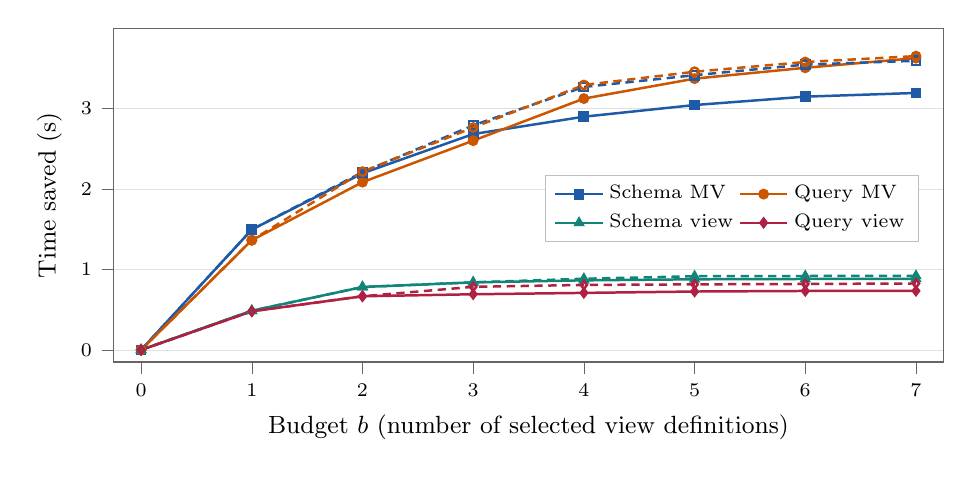
\begin{tikzpicture}
    \begin{axis}[
        tpchaxis,
        height=0.48\columnwidth,
        xlabel={Budget $b$ (number of selected view definitions)},
        ylabel={Time saved (s)},
        xmin=-0.25, xmax=7.25, ymin=-0.15, ymax=4.0,
        xtick={0,1,2,3,4,5,6,7}, ytick={0,1,2,3},
        legend style={font=\scriptsize, at={(0.97,0.46)}, anchor=east,
          legend columns=2, draw=black!25, inner xsep=3pt, inner ysep=1.5pt},
        legend cell align=left,
        every axis plot/.append style={line width=0.9pt, mark size=1.5pt},
    ]
    \addplot[tpchS, mark=square*] coordinates {(0,0) (1,1.496) (2,2.196) (3,2.684) (4,2.900) (5,3.045) (6,3.149) (7,3.195)};
    \addlegendentry{Schema MV}
    \addplot[tpchQ, mark=*] coordinates {(0,0) (1,1.364) (2,2.086) (3,2.602) (4,3.125) (5,3.373) (6,3.508) (7,3.628)};
    \addlegendentry{Query MV}
    \addplot[tpchS, densely dashed, mark=square, mark options={solid}, forget plot] coordinates {(0,0) (1,1.496) (2,2.210) (3,2.792) (4,3.270) (5,3.416) (6,3.548) (7,3.595)};
    \addplot[tpchQ, densely dashed, mark=o, mark options={solid}, forget plot] coordinates {(0,0) (1,1.364) (2,2.216) (3,2.765) (4,3.294) (5,3.459) (6,3.580) (7,3.653)};
    \addplot[tpchT, mark=triangle*] coordinates {(0,0) (1,0.487) (2,0.782) (3,0.840) (4,0.865) (5,0.878) (6,0.882) (7,0.884)};
    \addlegendentry{Schema view}
    \addplot[tpchR, mark=diamond*] coordinates {(0,0) (1,0.480) (2,0.667) (3,0.692) (4,0.709) (5,0.726) (6,0.733) (7,0.734)};
    \addlegendentry{Query view}
    \addplot[tpchT, densely dashed, mark=triangle, mark options={solid}, forget plot] coordinates {(0,0) (1,0.487) (2,0.782) (3,0.840) (4,0.885) (5,0.916) (6,0.919) (7,0.921)};
    \addplot[tpchR, densely dashed, mark=diamond, mark options={solid}, forget plot] coordinates {(0,0) (1,0.480) (2,0.667) (3,0.784) (4,0.808) (5,0.815) (6,0.820) (7,0.826)};
    \end{axis}
    \end{tikzpicture}
    \caption{Best workload saving per budget for every strategy family. Solid lines with filled marks are single-view rewrites; dashed lines with open marks are multi-view rewrites.}
    \Description{Workload runtime savings under different MV/view global budgets. Materialized views save up to 3.65 seconds, standard views below one second; schema-driven and query-driven curves nearly coincide.}
    \label{fig:tpch-budget-savings}
\end{figure}

Selection starts on the dimension side. The first picks are \texttt{N\_R} and \texttt{S\_N}, the TPC-H counterparts of the Gh and Ga folds. They replicate only small reference relations, refresh in milliseconds, and repay their maintenance within one workload pass ($\kappa_{\mathrm r}\le 1$); \texttt{N\_R} alone reaches $\Delta Q/\Delta M=227.35$. Fact-incident folds enter next and carry the bulk of the saving. Here \textsf{LineItem}, \textsf{Orders}, and \textsf{PartSupp} play the role of \textsf{Stats}: folds around them lift the saving to $3.60$\,s ($34.47\%$) at $b=7$ for multi-MV rewrites, but their refresh costs grow to tens of seconds.

Both effects saturate quickly. Savings flatten once the early picks cover the shared joins, around $b=4$--$6$, while $\Delta M$ keeps climbing with every wider fold. From $b=6$ onward even the refresh-aware selection of Fig.~\ref{fig:tpch-tradeoff} has $\Delta Q/\Delta M<1$: one refresh cycle costs more than one workload pass saves. Standard views mark the other extreme. They need no refresh, but they save at most $0.92$\,s (below $9\%$; Fig.~\ref{fig:tpch-budget-savings}). On TPC-H, as on \textsc{Sports}, the benefit lies in materializing the fold, not in the logical rewrite.

\noindent\emph{Takeaway.} The schema-driven principles transfer. Dimension-side folds are almost free and are picked first. Fact-incident folds buy the large savings, at redundancy and refresh costs that scale with the replicated fact rows. Whether they pay is a question of workload repetition, captured by $\kappa_{\mathrm r}$.

\begin{table}[t]
  \centering
  \caption{Best multi-MV selections per budget $b$: Workload saving $\Delta Q$, refresh cost $\Delta M$ in seconds, recoup ratio $\kappa_{\mathrm r}$ next to selected view IDs; bold marks the larger saving. Single-MV rewrites are dominated throughout, and standard views need no refresh but save at most $0.92$\,s (Fig.~\ref{fig:tpch-budget-savings}).}
  \label{tab:tpch-budgets}
  \small
  \setlength{\tabcolsep}{4pt}
  \begin{tabular}{c l l l l}
    \toprule
    $b$ & \multicolumn{2}{c}{Schema-driven} & \multicolumn{2}{c}{Query-driven} \\
    \cmidrule(lr){2-3}\cmidrule(lr){4-5}
    & $\Delta Q$/$\Delta M$/$\kappa_{\mathrm r}$ & View IDs & $\Delta Q$/$\Delta M$/$\kappa_{\mathrm r}$ & View IDs \\ \midrule
    1 & \textbf{1.50 / <0.01 / 1} & {\scriptsize $\mathbf{[3]}$} & 1.36 / 0.01 / 1 & {\scriptsize $[3]$} \\
    %\addlinespace[2pt]
    2 & 2.21 / 0.02 / 1 & {\scriptsize $[3,4]$} & \textbf{2.22 / 24.00 / 11} & {\scriptsize $\mathbf{[2,3]}$} \\
    %\addlinespace[2pt]
    3 & \textbf{2.79 / 10.76 / 4} & {\scriptsize $\mathbf{[2,3,4]}$} & 2.77 / 26.75 / 10 & {\scriptsize $[2,3,9]$} \\
    %\addlinespace[2pt]
    4 & 3.27 / 13.86 / 5 & {\scriptsize $[1,2,3,9]$} & \textbf{3.29 / 30.71 / 10}
      & {\scriptsize $\mathbf{[1,2,3,9]}$} \\
    5 & 3.42 / 25.70 / 8 & {\scriptsize $[1,2,3,8,9]$} & \textbf{3.46 / 32.47 / 10} & {\scriptsize $\mathbf{[1,2,3,9,12]}$} \\
    %\addlinespace[2pt]
    6 & 3.55 / 25.72 / 8 & {\scriptsize $[1,2,3,4,8,9]$} & \textbf{3.58 / 52.72 / 15} & {\scriptsize $\mathbf{[1,2,3,8,9,12]}$} \\
    %\addlinespace[2pt]
    7 & 3.60 / 32.11 / 9 & {\scriptsize $[1,2,3,4,7,8,9]$} & \textbf{3.65 / 52.92 / 15}
       & {\scriptsize $\mathbf{[1,2,3,4,8,9,12]}$} \\
    \bottomrule
  \end{tabular}
  \vspace{2pt}
  \begin{center}
  {\small \textit{Note:} IDs: 1=\texttt{O\_C}, 2=\texttt{L\_O\_C}, 3=\texttt{N\_R}, 4=\texttt{S\_N}, 7=\texttt{L\_O}, 8=\texttt{L\_O\_PS}, 9=\texttt{PS\_P}, 12=\texttt{L\_O\_C\_S\_N}$^{*}$; the asterisk marks a query-driven candidate.}
  \end{center}
\end{table}

\subsection{Query-Driven View Selection under Budget}\label{sec:tpch:query}

Query-driven denormalization treats the workload as evidence for missing E/R links. The predicates \texttt{C--S}, \texttt{L--S}, and \texttt{L--P} join relations that the schema connects only through longer foreign-key paths. Folding them promises exactly the joins the queries execute. Candidates that fold them, such as the asterisked \texttt{L\_O\_C\_S\_N} in Table~\ref{tab:tpch-budgets}, exist only in this enlarged space.

The enlarged space wins the query-only race, but narrowly and at a price. At $b=7$, the best query-driven multi-MV selection saves $3.65$\,s ($35.02\%$); its schema-driven counterpart saves $3.60$\,s ($34.47\%$). The margin is $0.05$\,s. The refresh cost, however, rises from $32.11$\,s to $52.92$\,s, and $\kappa_{\mathrm r}$ from $9$ to $15$. Small budgets show the same pattern. At $b=2$, the query-driven frontier gains $0.01$\,s but pays $\Delta M=24.00$\,s instead of $0.02$\,s: the wide \texttt{L\_O\_C} fold displaces the cheap dimension fold \texttt{S\_N}.

The cause is structural. The added links are fact-incident: \texttt{L--S} and \texttt{L--P} pull \textsf{LineItem}, the dominant fact table, into wider joins. The links that make query-driven candidates attractive thus also make them expensive to maintain; this is the TPC-H form of the fan-out effect behind RQ1. Fig.~\ref{fig:tpch-tradeoff} shows both refresh-aware frontiers: the query-driven curves match the schema-driven ones in saving but run consistently higher in refresh cost. Two further limits apply. Without materialization, the extra links add nothing; the best standard-view saving is $0.83$\,s, against $0.92$\,s schema-driven. Moreover, several of these predicates occur as semi- or anti-joins inside correlated subqueries ($Q_{16}$, $Q_{20}$, $Q_{22}$), which a materialized join cannot always serve.

\noindent\emph{Takeaway.} Workload-derived links extend the fold space legitimately, but they mostly add large fact-incident joins. Their maintenance grows faster than their marginal query benefit. Under refresh-aware selection, the schema-driven frontier remains the safer default; the query-driven one pays only when the workload repeats often enough between updates.

\begin{figure}[t]
    \centering
    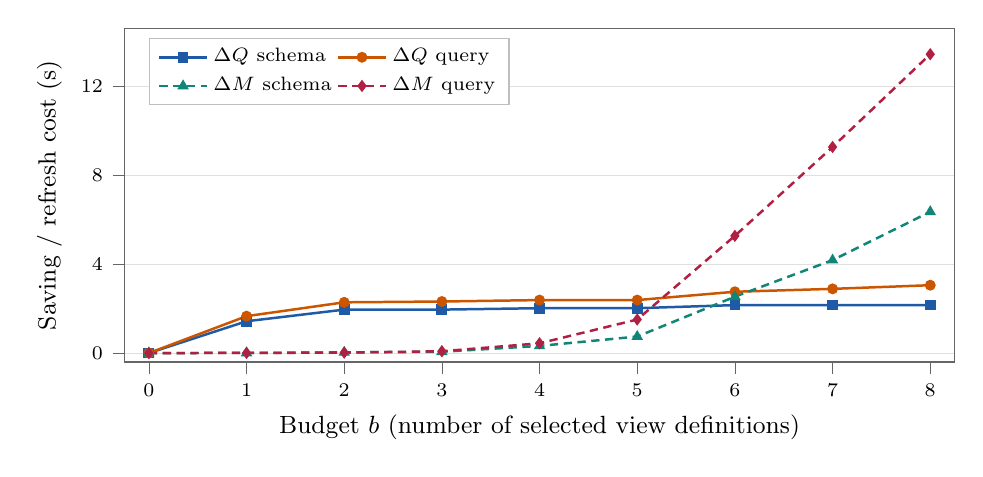
\begin{tikzpicture}
    \begin{axis}[
        tpchaxis,
        height=0.48\columnwidth,
        xlabel={Budget $b$ (number of selected view definitions)},
        ylabel={Saving / refresh cost (s)},
        xmin=-0.25, xmax=8.25, ymin=-0.4, ymax=14.6,
        xtick={0,1,2,3,4,5,6,7,8}, ytick={0,4,8,12},
        legend style={font=\scriptsize, at={(0.03,0.97)}, anchor=north west,
          legend columns=2, draw=black!25, inner xsep=3pt, inner ysep=1.5pt},
        legend cell align=left,
        every axis plot/.append style={line width=0.9pt, mark size=1.5pt},
    ]
    \addplot[tpchS, mark=square*] coordinates {(0,0) (1,1.430) (2,1.953) (3,1.953) (4,2.017) (5,2.017) (6,2.156) (7,2.156) (8,2.159)};
    \addlegendentry{$\Delta Q$ schema}
    \addplot[tpchQ, mark=*] coordinates {(0,0) (1,1.659) (2,2.281) (3,2.317) (4,2.382) (5,2.382) (6,2.756) (7,2.886) (8,3.050)};
    \addlegendentry{$\Delta Q$ query}
    \addplot[tpchT, densely dashed, mark=triangle*, mark options={solid}] coordinates {(0,0) (1,0.006) (2,0.029) (3,0.059) (4,0.321) (5,0.742) (6,2.534) (7,4.176) (8,6.350)};
    \addlegendentry{$\Delta M$ schema}
    \addplot[tpchR, densely dashed, mark=diamond*, mark options={solid}] coordinates {(0,0) (1,0.006) (2,0.022) (3,0.081) (4,0.439) (5,1.508) (6,5.268) (7,9.262) (8,13.432)};
    \addlegendentry{$\Delta M$ query}
    \end{axis}
    \end{tikzpicture}
    \caption{Refresh-aware trade-off: the per-pass query saving $\Delta Q$ (solid) against the refresh cost $\Delta M$ of one update cycle (dashed). From $b=6$ onward a refresh cycle costs more than a workload pass saves.}
    \Description{Line chart of query saving and total refresh cost per budget for schema-driven and query-driven selection. Savings stay between two and three seconds while refresh costs rise steeply beyond budget five, to 6.4 seconds schema-driven and 13.4 seconds query-driven.}
    \label{fig:tpch-tradeoff}
\end{figure}


\subsection{Discussion}\label{sec:tpch:discussion}

The TPC-H results confirm the framework in benchmark setting: the principles illustrated in \textsc{Sports} recurs in TPC-H. Redundancy and refresh are determined by the fact-incident folds, of \textsf{Stats} there and of \textsf{LineItem} and \textsf{PartSupp} here (RQ1). The large savings originate from a few widely shared folds around the fact table (RQ2). Dimension-side folds are picked first with marginal costs, Gh and Ga there, \texttt{N\_R} and \texttt{S\_N} here (RQ3). And the workload's canonical fold can lose operationally, through row grain there and selectivity here (RQ4).

$Q_2$ is the TPC-H witness: even for a single query, full folding is not monotone in benefit. Its join footprint is the chain \textsf{Part}--\textsf{PartSupp}--\textsf{Supplier}--\textsf{Nation}--\textsf{Region}, yet its full fold \texttt{PS\_S\_P\_N\_R} is the only evaluated configuration that \emph{loses} time ($-0.245$\,s). $Q_2$ restricts \textsf{Part} and \textsf{Region} with selective predicates and computes a correlated \texttt{MIN(ps\_supplycost)} subquery; the query-independent MV stores the join before these predicates apply and forfeits early filtering. Partial folds avoid the loss: the pair \texttt{N\_R} $\mid$ \texttt{PS\_S} matches the $0.211$\,s saving of the best single MV at a refresh cost of $0.843$\,s instead of $1.353$\,s. Exactly as the disclaimer of Sec.~\ref{sec:conceptual-view-selection} anticipates, a lattice projection need not be cheap.

TPC-H adds the recurring cost dimension. The recoup ratio $\kappa$ of Sec.~\ref{sec:case-exp} amortizes a one-time build; $\kappa_{\mathrm r}$ amortizes every refresh cycle. This reorders the answers: the query-driven frontier wins the pure query race yet loses the refresh-aware one. View selection on an evolving database is therefore a rate question: a fold is worth materializing when the workload repeats at least $\kappa_{\mathrm r}$ times per update cycle. The role of the algebra is to keep the candidate set for this test principled and small.

% \subsection{Schema-driven}

% \begin{comment}
% \begin{figure}[htbp]
%     \centering
%     \includegraphics[width=0.47\textwidth]{figures/schema_driven/trade_off_mv/budget_exact_tradeoff_lines.png}
%     \caption{Trade-off between Query and Refresh (Schema-driven)}
%     \Description{Trade-off between Query and Refresh (Schema-driven)}
%     \label{fig:trade_off_between_schema}
% \end{figure}

% \begin{table*}[htbp]
% \centering
% % \setlength{\tabcolsep}{6pt}
% % \renewcommand{\arraystretch}{1}
% \caption{Trade-off between Query Savings and Refresh Cost under Different Budgets (Schema-driven)}
% \label{tab:trade-off between best-case query savings schema}
% \resizebox{0.98\textwidth}{!}{
% \begin{tabular}{c c c c c c l}
% \hline
% $k$ & Q-Save (s) & R-Lost (s) & $r_k$ & Gain(\%) & Lost(\%) & MV Set \\
% \hline
% 0  & 0.0000 & 0.0000 & N/A      & 0.0  & 0.0    & \texttt{baseline} \\
% 1  & 1.4298 & 0.0063 & 227.35   & 14.6 & 0.6    & \texttt{N\_R} \\
% 2  & 1.9533 & 0.0287 & 68.03    & 19.9 & 2.8    & \texttt{N\_R}, \texttt{S\_N} \\
% 3  & 1.9533 & 0.0586 & 33.36    & 19.9 & 5.6    & \texttt{N\_R}, \texttt{S\_N}, \texttt{S\_N\_R} \\
% 4  & 2.0169 & 0.3206 & 6.29     & 20.5 & 30.8   & \texttt{N\_R}, \texttt{S\_N}, \texttt{S\_N\_R}, \texttt{C\_N} \\
% 5  & 2.0169 & 0.7424 & 2.72     & 20.5 & 71.4   & \texttt{N\_R}, \texttt{S\_N}, \texttt{S\_N\_R}, \texttt{C\_N}, \texttt{C\_N\_R} \\
% 6  & 2.1555 & 2.5342 & 0.85     & 21.9 & 243.8  & \texttt{N\_R}, \texttt{S\_N}, \texttt{S\_N\_R}, \texttt{C\_N}, \texttt{C\_N\_R}, \texttt{PS\_P} \\
% 7  & 2.1555 & 4.1756 & 0.52     & 21.9 & 401.7  & \texttt{N\_R}, \texttt{S\_N}, \texttt{S\_N\_R}, \texttt{C\_N}, \texttt{C\_N\_R}, \texttt{PS\_P}, \texttt{PS\_S} \\
% 8  & 2.1593 & 6.3498 & 0.34     & 22.0 & 610.8  & \texttt{N\_R}, \texttt{S\_N}, \texttt{S\_N\_R}, \texttt{C\_N}, \texttt{C\_N\_R}, \texttt{PS\_P}, \texttt{PS\_S}, \texttt{PS\_S\_N} \\
% 9  & 2.2637 & 8.9901 & 0.25     & 23.0 & 864.8  & \texttt{N\_R}, \texttt{S\_N}, \texttt{S\_N\_R}, \texttt{C\_N}, \texttt{C\_N\_R}, \texttt{PS\_P}, \texttt{PS\_S}, \texttt{PS\_S\_N}, \texttt{PS\_S\_N\_R} \\
% 10 & 2.2637 & 11.3358 & 0.20    & 23.0 & 1090.5 & \texttt{N\_R}, \texttt{S\_N}, \texttt{S\_N\_R}, \texttt{C\_N}, \texttt{C\_N\_R}, \texttt{PS\_P}, \texttt{PS\_S}, \texttt{PS\_S\_N}, \texttt{PS\_S\_N\_R}, \texttt{PS\_S\_P} \\
% \hline
% \end{tabular}
% }
% \end{table*}
% \end{comment}


% \subsection{Query-driven}

% \begin{comment}
% \begin{table*}[htbp]
% \centering
% % \setlength{\tabcolsep}{2pt}
% % \renewcommand{\arraystretch}{1}
% \caption{Trade-off between Query Savings and Refresh Cost under Different Budgets (Query-driven)}
% \label{tab:trade_off_between_best_case_query_savings_query}
% \resizebox{0.98\textwidth}{!}{
% \begin{tabular}{r l l l l l l}
% \hline
% $k$ & Q-Save (s) & R-Lost (s) & $r_k$ & Gain(\%) & Lost(\%) & MV Set \\
% \hline
% 0  & 0.0000 & 0.0000 & N/A     & 0.0 & 0.0    & \texttt{baseline} \\
% 1  & 1.6593 & 0.0054 & 306.67 & 14.9 & 0.3   & \texttt{N\_R} \\
% 2  & 2.2809 & 0.0141 & 162.02 & 20.5 & 0.9   & \texttt{N\_R}, \texttt{S\_N} \\
% 3  & 2.3173 & 0.0376 & 61.569  & 20.8 & 2.3   & \texttt{N\_R}, \texttt{S\_N}, \texttt{S\_N\_R} \\
% 4  & 2.3173 & 0.5410 & 4.2831   & 20.8 & 33.3  & \texttt{N\_R}, \texttt{S\_N}, \texttt{S\_N\_R}, \texttt{C\_N\_R} \\
% 5  & 2.3822 & 1.1053 & 2.1551   & 21.4 & 68.1  & \texttt{N\_R}, \texttt{S\_N}, \texttt{S\_N\_R}, \texttt{C\_N\_R}, \texttt{C\_N} \\
% 6  & 2.3932 & 3.1109 & 0.7693   & 21.5 & 191.7 & \texttt{N\_R}, \texttt{S\_N}, \texttt{S\_N\_R}, \texttt{C\_N\_R}, \texttt{C\_N}, \texttt{PS\_S} \\
% 7  & 2.5456 & 5.5262 & 0.4606   & 22.8 & 340.5 & \texttt{N\_R}, \texttt{S\_N}, \texttt{S\_N\_R}, \texttt{C\_N\_R}, \texttt{C\_N}, \texttt{PS\_S}, \texttt{PS\_P} \\
% 8  & 2.9159 & 8.7794 & 0.3321   & 26.2 & 541.0 & \texttt{N\_R}, \texttt{S\_N}, \texttt{S\_N\_R}, \texttt{C\_N\_R}, \texttt{C\_N}, \texttt{PS\_S}, \texttt{PS\_P}, \texttt{L\_O\_C\_S}$^{*}$ \\
% 9  & 3.0457 & 12.7022 & 0.2398  & 27.3 & 782.7 & \texttt{N\_R}, \texttt{S\_N}, \texttt{S\_N\_R}, \texttt{C\_N\_R}, \texttt{C\_N}, \texttt{PS\_S}, \texttt{PS\_P}, \texttt{L\_O\_C\_S}$^{*}$, \texttt{L\_O\_C\_S\_N1\_N2\_R}$^{*}$ \\
% 10 & 3.0496 & 16.3091 & 0.1870  & 27.3 & 1005.0 & \texttt{N\_R}, \texttt{S\_N}, \texttt{S\_N\_R}, \texttt{C\_N\_R}, \texttt{C\_N}, \texttt{PS\_S}, \texttt{PS\_P}, \texttt{L\_O\_C\_S}$^{*}$, \texttt{L\_O\_C\_S\_N1\_N2\_R}$^{*}$, \texttt{L\_O\_C\_S\_N}$^{*}$ \\
% \hline
% \end{tabular}
% }
% \end{table*}
% \end{comment}


% \begin{figure}[htbp]
%     \centering
%     \includegraphics[width=0.47\textwidth]{figures/query_driven/trade_off_new/budget_exact_tradeoff_lines.png}
%     \caption{Trade-off between Query and Refresh (Query-driven)}
%     \Description{Trade-off between Query and Refresh (Query-driven)}
%     \label{fig:trade_off-query}
% \end{figure}







\begin{comment}
\clearpage

\section{Experiments on TPC-H (\textcolor{red}{Version 1})}\label{app:tpch}
The fully enumerated \textsc{Sports} study in Sec.~\ref{sec:case-exp} identified materialized row grain as the main driver of redundancy and query cost, with lattice meet and join bracketing workload choices. TPC-H tests these principles on a larger link set under selective predicates, aggregation, correlated subqueries, and recurring refresh costs. We construct folds, compare reusable query savings with maintenance, and examine when full folding fails.

\subsection{Applying the Algebra to TPC-H}

By the theorem in Sec.~\ref{sec:boolean}, TPC-H's eight primary-key/foreign-key links yield $2^8=256$ schema-driven Join Views. The query-driven method builds on these folds but does not enlarge their Boolean algebra: it adds \texttt{C--S}, \texttt{L--S}, and \texttt{L--P}, the only non-schema predicate types among the 20 join-containing queries. Candidates are generated from query-specific occurrence graphs, where repeated roles are distinct vertices. For example, \texttt{N1} and \texttt{N2} both represent \texttt{NATION}. These augmented graphs support customized views and rewrites but need not themselves form an E/R Boolean algebra.

We translate each candidate into canonical SQL using a spanning tree and the occurrence order \texttt{LineItem(L)}, \texttt{Orders(O)}, \texttt{Customer (C)}, \texttt{PartSupp(PS)}, \texttt{Supplier(S)}, \texttt{Part(P)}, \texttt{Nation(N)}, \texttt{N1}, \texttt{N2}, \texttt{Region(R)}. Non-tree predicates are retained, while PostgreSQL chooses the physical plan. Schema-style candidates containing \texttt{Customer--Orders} are rooted at \texttt{Customer} and use left joins throughout the \texttt{Orders} branch to preserve customers without orders. Elsewhere, inner joins are used canonically because non-null foreign keys make the corresponding inner and outer joins result-equivalent. Query-style candidates use inner joins, except the \texttt{Orders--Customer} candidates for Q13 and Q22, whose full outer join is equivalent to \texttt{Customer LEFT JOIN Orders} under the non-null foreign-key constraint. Different occurrences, predicates, join types, columns, or indexes define distinct physical candidates.

Views retain all joined columns, bag multiplicities, and null-extended rows without duplicate elimination or pre-aggregation. Rewrites restore query semantics using null-key filters, \texttt{DISTINCT}, grouping, aggregates, or correlated subqueries as needed. Before timing, we compare sorted complete outputs with the normalized baseline for the first parameter binding. This check ensures result and logical equivalence between each rewrite and the normalized baseline.

\subsection{Reproducibility}
Experiments use TPC-H at SF$\,=\,0.5$ on PostgreSQL~18.2 and Red Hat Enterprise Linux~8.10, with two AMD EPYC 7742 processors, 1.0\,TiB RAM, and NVMe RAID10 storage. A private DBGEN derivative based on TPC-H Parameter Substitution v.3.0.0 generates the data. Relevant primary- and foreign-key columns, including composite-key components, are indexed. In one warm-cache session, each baseline and rewrite receives ten warm-up runs on its first binding and up to 100 timed bindings (seed 20260101), stopping after ten consecutive runs above 1.5\,s. We report the arithmetic mean of the central 60\% of client times. For each indexed MV, the post-insert and post-delete \texttt{REFRESH MATERIALIZED VIEW} invocations are each timed once in \texttt{psql}, including index maintenance.

We test materialized and standard views with single- and multi-view rewrites. Budget $b$ limits the number of selected view definitions. For single-view rewrites, candidates dominated across their per-query runtime vectors are pruned before exact enumeration. Multi-view frontiers are solved exactly by a binary integer program over beneficial rewrite templates. Each query uses its fastest beneficial enabled rewrite or the normalized baseline, and the selected set minimizes workload runtime. We report workload saving $\Delta Q$, recurring refresh cost $\Delta M$, and, for $\Delta Q>0$, refresh payback $\kappa_{\mathrm{r}}=\lceil\Delta M/\Delta Q\rceil$. Beneficial standard views have $\kappa_{\mathrm{r}}=0$, while for $\Delta Q\leq0$ it is undefined. This recurring-refresh metric is not directly comparable to the earlier build-payback $\kappa$.

\subsection{Budgeted View Selection}

With TPC-H's larger candidate set, budget $b$ poses the small-set question from Sec.~\ref{sec:conceptual-view-selection}: how much of the workload can $b$ globally shared views support?

\begin{figure}[htbp]
    \centering
    \includegraphics[width=\columnwidth]{figures/mix_query_schema_driven/all_budget_tradeoff_saved_time.png}
    \caption{Query Savings Under Different MV/View Budgets}
    \Description{Workload Runtime Savings Under Different MV/View Global Budgets}
    \label{fig:runtime_saving_under_different_mv_v_budgets}
\end{figure}


\definecolor{viewset}{RGB}{232,245,233}    % light green
% \definecolor{viewset}{RGB}{243,229,245}    % light purple
% \definecolor{viewset}{RGB}{255,235,238}    % light pink
% \definecolor{viewset}{RGB}{245,245,245}    % light gray

\begin{table*}[htbp]
\centering
\caption{Best workload savings, refresh losses, and $\kappa_{\mathrm{r}}$ under different MV and view budgets}
\label{tab:best_saving_all_budgets}
\resizebox{0.98\textwidth}{!}{
\begin{tabular}{c c c c c c c c c}
\toprule
& \multicolumn{4}{c}{Materialized View (precomputed data)}
& \multicolumn{4}{c}{View (not precomputed)} \\
\cmidrule(lr){2-5}
\cmidrule(lr){6-9}

& \multicolumn{2}{c}{Schema-driven}
& \multicolumn{2}{c}{Query-driven}
& \multicolumn{2}{c}{Schema-driven}
& \multicolumn{2}{c}{Query-driven} \\
\cmidrule(lr){2-3}
\cmidrule(lr){4-5}
\cmidrule(lr){6-7}
\cmidrule(lr){8-9}

$b$ & MV & Multi-MV & MV & Multi-MV
& View & Multi-View & View & Multi-View \\
\midrule
0
& 0.00s / 0.00s / --
& 0.00s / 0.00s / --
& 0.00s / 0.00s / --
& 0.00s / 0.00s / --
& 0.00s / 0.00s / --
& 0.00s / 0.00s / --
& 0.00s / 0.00s / --
& 0.00s / 0.00s / -- \\

1
& \textbf{1.50s / $<$0.01s / 1}
& \textbf{1.50s / $<$0.01s / 1}
& 1.36s / 0.01s / 1
& 1.36s / 0.01s / 1
& 0.49s / 0.00s / 0
& 0.49s / 0.00s / 0
& 0.48s / 0.00s / 0
& 0.48s / 0.00s / 0 \\
\rowcolor{viewset}
&
$\mathbf{[3]}$
& $\mathbf{[3]}$
& $[3]$
& $[3]$
& $[6]$
& $[6]$
& $[5]$
& $[5]$ \\


2
& 2.20s / 0.02s / 1
& 2.21s / 0.02s / 1
& 2.09s / 24.00s / 12
& \textbf{2.22s / 24.00s / 11}
& 0.78s / 0.00s / 0
& 0.78s / 0.00s / 0
& 0.67s / 0.00s / 0
& 0.67s / 0.00s / 0 \\
\rowcolor{viewset}
&
$[3,4]$
& $[3,4]$
& $[2,3]$
& $\mathbf{[2,3]}$
& $[1,6]$
& $[1,6]$
& $[1,5]$
& $[1,5]$ \\


3
& 2.68s / 10.76s / 5
& \textbf{2.79s / 10.76s / 4}
& 2.60s / 24.19s / 10
& 2.77s / 26.75s / 10
& 0.84s / 0.00s / 0
& 0.84s / 0.00s / 0
& 0.69s / 0.00s / 0
& 0.78s / 0.00s / 0 \\
\rowcolor{viewset}
&
$[2,3,4]$
& $\mathbf{[2,3,4]}$
& $[2,3,4]$
& $[2,3,9]$
& $[1,6,7]$
& $[1,6,7]$
& $[1,5,11]$
& $[1,4,5]$ \\


4
& 2.90s / 14.05s / 5
& 3.27s / 13.86s / 5
& 3.13s / 27.83s / 9
& \textbf{3.29s / 30.71s / 10}
& 0.87s / 0.00s / 0
& 0.89s / 0.00s / 0
& 0.71s / 0.00s / 0
& 0.81s / 0.00s / 0 \\
\rowcolor{viewset}
&
$[1,2,3,10]$
& $[1,2,3,9]$
& $[2,4,12,13]$
& $\mathbf{[1,2,3,9]}$
& $[1,4,6,7]$
& $[1,4,6,7]$
& $[1,5,10,11]$
& $[1,4,5,11]$ \\


5
& 3.05s / 25.89s / 9
& 3.42s / 25.70s / 8
& 3.37s / 33.78s / 11
& \textbf{3.46s / 32.47s / 10}
& 0.88s / 0.00s / 0
& 0.92s / 0.00s / 0
& 0.73s / 0.00s / 0
& 0.82s / 0.00s / 0 \\
\rowcolor{viewset}
&
$[1,2,3,8,10]$
& $[1,2,3,8,9]$
& $[1,2,10,12,13]$
& $\mathbf{[1,2,3,9,12]}$
& $[1,4,6,7,8]$
& $[1,2,4,6,7]$
& $[1,5,10,11,13]$
& $[1,2,4,5,11]$ \\


6
& 3.15s / 27.25s / 9
& 3.55s / 25.72s / 8
& 3.51s / 39.36s / 12
& \textbf{3.58s / 52.72s / 15}
& 0.88s / 0.00s / 0
& 0.92s / 0.00s / 0
& 0.73s / 0.00s / 0
& 0.82s / 0.00s / 0 \\
\rowcolor{viewset}
&
$[1,2,3,8,10,14]$
& $[1,2,3,4,8,9]$
& $[1,2,10,12,13,14]$
& $\mathbf{[1,2,3,8,9,12]}$
& $[1,2,4,6,7,8]$
& $[1,2,4,6,7,9]$
& $[1,2,5,10,11,13]$
& $[1,2,4,5,11,16]$ \\


7
& 3.20s / 33.64s / 11
& 3.60s / 32.11s / 9
& 3.63s / 59.61s / 17
& \textbf{3.65s / 52.92s / 15}
& 0.88s / 0.00s / 0
& 0.92s / 0.00s / 0
& 0.73s / 0.00s / 0
& 0.83s / 0.00s / 0 \\
\rowcolor{viewset}
&
$[1,2,3,7,8,10,14]$
& $[1,2,3,4,7,8,9]$
& $[1,2,8,10,12,13,14]$
& $\mathbf{[1,2,3,4,8,9,12]}$
& $[1,2,4,6,7,8,9]$
& $[1,2,4,6,7,9,15]$
& $[1,2,5,10,11,13,17]$
& $[1,2,4,5,7,11,15]$ \\

\bottomrule
\end{tabular}
}
\begin{center}
{\small\textit{Note:} Entries report
$\Delta Q/\Delta M/\kappa_{\mathrm r}$. Green-shaded rows give the
candidate IDs of the view set selected for each strategy. Boldface marks the largest $\Delta Q$ at each cardinality.}
\end{center}
\end{table*}























\begin{table}[htbp]
\centering
\caption{Mapping between view candidates and their IDs}
\label{tab:mapping_between_view_candidates_and_their_ids}
\resizebox{\columnwidth}{!}{%
\begin{tabular}{c l c l c l}
\hline
ID & View (Count)
& ID & View (Count)
& ID & View (Count) \\
\hline

1  & \texttt{O\_C} (39)
& 7  & \texttt{L\_O} (13)
& 13 & \texttt{L\_O\_C\_S\_N1\_N2\_R}$^{*}$ (7) \\

2  & \texttt{L\_O\_C} (32)
& 8  & \texttt{L\_O\_PS} (12)
& 14 & \texttt{PS\_S\_N\_R} (4) \\

3  & \texttt{N\_R} (24)
& 9  & \texttt{PS\_P} (12)
& 15 & \texttt{C\_N} (2) \\

4  & \texttt{S\_N} (22)
& 10 & \texttt{PS\_S\_N} (11)
& 16 & \texttt{O\_C\_N\_R} (1) \\

5  & \texttt{L\_PS} (14)
& 11 & \texttt{L\_S\_P}$^{*}$ (9)
& 17 & \texttt{O\_C\_S\_N\_R}$^{*}$ (1) \\

6  & \texttt{L\_PS\_S\_P\_N} (14)
& 12 & \texttt{L\_O\_C\_S\_N}$^{*}$ (7)
&    & \\

\hline
\end{tabular}
}
\begin{center}
{\small \textit{Note:} Count is frequency. Asterisk ($^{*}$) marks query-driven candidates.}
\end{center}
\end{table}





Figure~\ref{fig:runtime_saving_under_different_mv_v_budgets} and Table~\ref{tab:best_saving_all_budgets} share the normalized-workload baseline $T_0=10.4312$\,s. Table~\ref{tab:mapping_between_view_candidates_and_their_ids} decodes the candidate IDs. At $b=7$, query-driven multi-MVs save $3.65$\,s ($35.02\%$, $\kappa_{\mathrm{r}}=15$), versus $3.60$\,s ($34.47\%$, $\kappa_{\mathrm{r}}=9$) for schema-driven multi-MVs: only $0.05$\,s more query saving at greater refresh exposure.

Standard views avoid refresh but save at most about $0.92$\,s (below $9\%$). MV gains flatten around $b=4$--$6$ once common joins are covered. Later query-specific candidates add little saving.

\subsection{Query Savings versus Refresh Cost}

Refresh-aware frontiers consider both query saving $\Delta Q_b$ and refresh cost $\Delta M_b$, with $\Delta M_b$ approximated by summing the independently measured post-insert and post-delete full-refresh times of the selected MVs. The batch contains 70 \texttt{Customer}, 100 \texttt{Part}, 400 \texttt{PartSupp}, 750 \texttt{Orders}, and 2,981 \texttt{LineItem} tuples. At SF$\,=\,0.5$, \texttt{Nation} and \texttt{Region} are static, and \texttt{Supplier} receives no update tuple. Within a candidate pool pre-filtered by standalone net benefit, exact size-$b$ enumeration retains the set maximizing $r_b=\Delta Q_b/\Delta M_b$. For $\Delta Q_b>0$ and $\Delta M_b>0$, $\kappa_{\mathrm r}=\lceil1/r_b\rceil$ is computed from unrounded measurements.


\begin{figure}[htbp]
    \centering
    \includegraphics[width=0.47\textwidth]
    {figures/mix_query_schema_driven/combined_budget_exact_tradeoff_lines.png}
    \caption{Trade-off between query savings and refresh cost}
    \Description{A combined line chart compares schema-driven solid lines and query-driven dashed lines for query-time savings and insertion, deletion, and total refresh costs as the materialized-view budget increases.}
    \label{fig:trade_off_combined}
\end{figure}

At small budgets, Fig.~\ref{fig:trade_off_combined} shows that the refresh-aware frontier selects the compact dimension folds \texttt{N\_R} and then \texttt{S\_N}. For \texttt{N\_R}, $r_1=227.35$ under schema-driven and $306.67$ under query-driven selection. These folds are cheap to recompute because the relations are small. The update batch contains no \texttt{Nation}, \texttt{Region}, or \texttt{Supplier} tuples, although the measurements conservatively charge full refreshes. Later selections increasingly involve larger relations such as \texttt{PartSupp}, \texttt{Orders}, and \texttt{LineItem}, so refresh grows faster than marginal saving. From $b=6$ onward, $r_b<1$ in both settings. Thus workload repetition determines whether broad folds amortize maintenance. Q2 next tests full folding before maintenance is charged.


\subsection{TPC-H Q2: When Full Folding Hurts}

Q2 sharpens the operational gap exposed by RQ4 in Sec.~\ref{sec:exp:meetjoin}: even the canonical full fold for one query can lose once selectivity and a correlated aggregate shape the physical plan. Its join footprint is the chain \texttt{Part}--\texttt{PartSupp}--\texttt{Supplier}--\texttt{Nation}--\texttt{Region}, suggesting \texttt{PS\_S\_P\_N\_R}. Yet Q2 combines selective predicates on \texttt{Part} and \texttt{Region} with a correlated \texttt{MIN(ps\_supplycost)} subquery. Because a query-independent MV stores the join before these predicates are applied, the full fold materializes unfiltered rows. Its observed slowdown is consistent with forfeiting early filtering.

\begin{table}[htbp]
\centering
\caption{Q2 cost--benefit by MV configuration}
\label{tab:mv_cost_benefit}
\resizebox{\columnwidth}{!}{%
\begin{tabular}{clcccc@{\hspace{5pt}}ccc}
\toprule
& & & \multicolumn{3}{c}{Schema-driven}
& \multicolumn{3}{c}{Query-driven} \\
\cmidrule(lr){4-6}\cmidrule(lr){7-9}
$i$ & View & Red.
& Q-Saved & R-Cost & $\kappa_{\mathrm{r}}$
& Q-Saved & R-Cost & $\kappa_{\mathrm{r}}$ \\
\midrule
\rowcolor{singleviewbg} 0 & $\varnothing$ & 1.000 & 0.000 & 0.000 & -- & 0.000 & 0.000 & -- \\
\rowcolor{singleviewbg} 1 & \texttt{N\_R} & 1.000 & +0.107 & 0.003 & 1 & +0.103 & 0.013 & 1 \\
\rowcolor{singleviewbg} 2 & \texttt{S\_N} & 1.000 & +0.077 & 0.012 & 1 & +0.085 & 0.195 & 3 \\
\rowcolor{singleviewbg} 3 & \texttt{PS\_P} & 1.046 & +0.075 & 0.910 & 13 & +0.067 & 2.755 & 42 \\
\rowcolor{singleviewbg} 4 & \texttt{PS\_S} & 1.047 & +0.036 & 0.840 & 24 & +0.043 & 2.156 & 51 \\
\rowcolor{singleviewbg} 5 & \texttt{S\_N\_R} & 1.001 & +0.098 & 0.016 & 1 & +0.092 & 0.053 & 1 \\
\rowcolor{singleviewbg} 6 & \texttt{PS\_S\_N} & 1.075 & +0.064 & 1.100 & 18 & +0.070 & 2.192 & 32 \\
\rowcolor{singleviewbg} 7 & \texttt{PS\_S\_P} & 1.094 & +0.014 & 1.181 & 86 & +0.041 & 2.095 & 52 \\
\rowcolor{singleviewbg} 8 & \texttt{PS\_S\_N\_R} & 1.096 & +0.211 & 1.353 & 7 & +0.205 & 5.579 & 28 \\
\rowcolor{singleviewbg} 9 & \texttt{PS\_S\_P\_N} & 1.121 & +0.146 & 1.507 & 11 & +0.137 & 4.720 & 35 \\
\rowcolor{singleviewbg} 10 & \texttt{PS\_S\_P\_N\_R} & 1.142 & -0.245 & 1.605 & -- & -0.282 & 1.461 & -- \\
\midrule
\rowcolor{multiviewbg} 1+3 & \texttt{N\_R $\mid$ PS\_P} & 1.046 & +0.185 & 0.913 & 5 & +0.160 & 2.768 & 18 \\
\rowcolor{multiviewbg} 1+4 & \texttt{N\_R $\mid$ PS\_S} & 1.047 & +0.211 & 0.843 & 4 & +0.202 & 2.170 & 11 \\
\rowcolor{multiviewbg} 3+2 & \texttt{PS\_P $\mid$ S\_N} & 1.047 & +0.185 & 0.922 & 5 & +0.159 & 2.949 & 19 \\
\rowcolor{multiviewbg} 1+7 & \texttt{N\_R $\mid$ PS\_S\_P} & 1.094 & +0.073 & 1.184 & 17 & +0.008 & 2.109 & 251 \\
\rowcolor{multiviewbg} 3+5 & \texttt{PS\_P $\mid$ S\_N\_R} & 1.047 & +0.186 & 0.926 & 5 & +0.167 & 2.808 & 17 \\
\bottomrule
\end{tabular}}
\begin{center}
\textit{Note:} Positive Q-Saved means faster. Negative means slower.
\end{center}
\end{table}

In Table~\ref{tab:mv_cost_benefit}, Q-Saved and R-Cost are seconds, Red.\ is the ratio from Sec.~\ref{sec:exp:setup}, and a dash denotes non-positive saving. For schema-driven realizations, the full fold is $0.245$\,s slower than baseline, whereas the best single partial fold, \texttt{PS\_S\_N\_R}, saves $0.211$\,s with refresh cost $1.353$\,s and $\kappa_{\mathrm r}=7$. Thus, seven executions of Q2 are required to amortize one update-maintenance cycle. The pair \texttt{N\_R $\mid$ PS\_S} gives essentially the same saving with refresh cost $0.843$\,s and $\kappa_{\mathrm r}=4$. However, it leaves the \texttt{S--N} link unfolded and therefore does not have the same edge coverage as \texttt{PS\_S\_N\_R}. This is not a controlled split-versus-single comparison and cannot establish that splitting itself is better. It shows only that smaller partial folds are more suitable among the evaluated Q2 realizations.

\noindent\emph{Cross-benchmark takeaway} The \textsc{Sports} principles carry over: the Boolean algebra supplies a principled candidate space, while row grain, reuse, and refresh cost determine which candidates are operationally worthwhile. Reuse compact shared folds and materialize broad fact-incident folds only when repeated workloads amortize maintenance. Workload-derived links enlarge the choice set without changing these rules.
\end{comment}






\section{Conclusion and Future Work}\label{sec:conclusion}

Starting from the observation that E/R links represent principled degrees of data redundancy already during the conceptual design of database schemata, our research has established Boolean algebras of (de-)normalized Entity/Relationship diagrams and Join Views. Operations of join, meet, and negation provide conceptual insight which selections of join views are appropriate for a given workload of join queries. Experiments with our running example and the TPC-H benchmark have illustrated how principles from our conceptual framework apply to view selection at logical and operational level.

Future work may focus on several directions: a) investigate our framework on more relational datasets with specific workloads, b) apply the framework to other data models at logical and physical level, or c) extend the approach to dynamic view selection.

\section*{Artifacts}

The source code, experimental scripts, documents and instructions on how to reproduce the results from our research can be found under https://github.com/denormalizationexp/denormalizationExp.git.

























%%
%% The next two lines define the bibliography style to be used, and
%% the bibliography file.
\bibliographystyle{ACM-Reference-Format}
\bibliography{references}

%%
%% If your work has an appendix, this is the place to put it.
%\appendix

%\section{Research Methods}






\appendix
\begin{comment}


\section{TPC-H}
We use the TPC-H database and query workload to evaluate the performance impact of different denormalization configurations.

\end{comment}

\begin{comment}
TPC-H is a widely used decision support benchmark designed to evaluate the performance of analytical query processing systems. It models a business-oriented data warehouse environment and consists of a suite of complex queries and large-scale relational tables.
\end{comment}

\begin{comment}
\subsection{TPC-H Benchmark}

The TPC-H database consists of eight base relations: \texttt{Region}, \texttt{Nation}, \texttt{Customer}, \texttt{Orders}, \texttt{LineItem}, \texttt{Supplier}, \texttt{Part}, and \texttt{PartSupp}, as shown in Figure~\ref{fig:schema_driven_graph}. Each edge represents a primary-key and foreign-key relationship between two relations. The benchmark is parameterized by a scale factor $sf$, which determines the size of the generated instance. Table~\ref{tab:tpch_schema_new} provides an overview of the TPC-H relations at scale factor 0.5, including the number of attributes, cardinalities, row counts, and key constraints. At this scale factor, the dataset size is approximately 0.5 GB. Primary-key attributes are shown in bold, while foreign-key attributes are underlined. Figure~\ref{fig:query_driven_graph} extends the schema graph with workload-derived relationships identified from the TPC-H query workload, shown as dashed edges.


\begin{figure}[htbp]
    \centering

    \begin{subfigure}[b]{0.48\linewidth}
        \centering
        \includegraphics[width=\linewidth]{figures/tpch_database/tpch_schema_graph.png}
        \caption{Schema-driven}
        \label{fig:schema_driven_graph}
    \end{subfigure}
    \hfill
    \begin{subfigure}[b]{0.48\linewidth}
        \centering
        \includegraphics[width=\linewidth]{figures/tpch_database/tpch_schema_graph_query.png}
        \caption{Query-driven}
        \label{fig:query_driven_graph}
    \end{subfigure}

    \caption{Comparison of schema-driven and query-driven diagram for TPC-H.}

    \Description{schema-driven and query-driven}

    \label{fig:tpch_driven_graphs}
\end{figure}


\begin{comment}
\begin{table*}[htbp]
\centering
\setlength{\tabcolsep}{5pt}
\renewcommand{\arraystretch}{1}
\caption{TPC-H Schema Overview and Key Constraints (SF = 0.5)}
\label{tab:tpch_schema_new}
\resizebox{0.95\textwidth}{!}{
\begin{tabular}{l p{8cm} l p{4cm}}
\hline
\textbf{Table} & \textbf{Attributes} & \textbf{Primary Key} & \textbf{Foreign Keys} \\
\hline

region (5)
& regionkey, name, comment
& regionkey
& -- \\

nation (25)
& nationkey, name, regionkey, comment
& nationkey
& regionkey $\rightarrow$ region \\

supplier (5K)
& suppkey, name, address, nationkey, phone, acctbal, comment
& suppkey
& nationkey $\rightarrow$ nation \\

customer (75K)
& custkey, name, address, nationkey, phone, acctbal, mktsegment, comment
& custkey
& nationkey $\rightarrow$ nation \\

part (100K)
& partkey, name, mfgr, brand, type, size, container, retailprice, comment
& partkey
& -- \\

partsupp (400K)
& partkey, suppkey, availqty, supplycost, comment
& (partkey, suppkey)
& partkey $\rightarrow$ part \newline suppkey $\rightarrow$ supplier \\

orders (750K)
& orderkey, custkey, orderstatus, totalprice, orderdate, orderpriority, clerk, shippriority, comment
& orderkey
& custkey $\rightarrow$ customer \\

lineitem (3M)
& orderkey, partkey, suppkey, linenumber, quantity, extendedprice, discount, tax, returnflag, linestatus, shipdate, commitdate, receiptdate, shipinstruct, shipmode, comment
& (orderkey, linenumber)
& orderkey $\rightarrow$ orders \newline (partkey, suppkey) $\rightarrow$ partsupp \\

\hline
\end{tabular}
}
\end{table*}
\end{comment}

\begin{comment}
\begin{table}[htbp]
\centering
\small
\setlength{\tabcolsep}{5pt}
\renewcommand{\arraystretch}{1.05}
\caption{TPC-H schema overview (SF\,=\,0.5). Primary keys in \textbf{bold}, foreign keys \underline{underlined} (a shared underline marks a composite foreign key).}
\label{tab:tpch_schema_new}
\begin{tabular}{@{}l p{6cm}@{}}
\toprule
\textbf{Table (rows)} & \textbf{Attributes} \\
\midrule
region (5)      & \textbf{regionkey}, name, comment \\
nation (25)     & \textbf{nationkey}, name, \underline{regionkey}, comment \\
supplier (5K)   & \textbf{suppkey}, name, address, \underline{nationkey}, phone, acctbal, comment \\
customer (75K)  & \textbf{custkey}, name, address, \underline{nationkey}, phone, acctbal, mktsegment, comment \\
part (0.1M)     & \textbf{partkey}, name, mfgr, brand, type, size, container, retailprice, comment \\
partsupp (0.4M) & \textbf{(\underline{partkey}, \underline{suppkey})}, availqty, supplycost, comment \\
orders (0.75M)  & \textbf{orderkey}, \underline{custkey}, orderstatus, totalprice, orderdate, orderpriority, clerk, shippriority, comment \\
lineitem (3M)   & \textbf{(\underline{orderkey}, linenumber)}, \underline{partkey, suppkey}, quantity, extendedprice, discount, tax, returnflag, linestatus, shipdate, commitdate, receiptdate, shipinstruct, shipmode, comment \\
\bottomrule
\end{tabular}
\end{table}


\begin{table*}[t]
\centering
% \scriptsize
% \setlength{\tabcolsep}{2.2pt}
% \renewcommand{\arraystretch}{0.9}
\caption{TPC-H Query Schema \textcolor{red}{Warning: Q20}}
\label{tab:query_schema}
\resizebox{0.97\textwidth}{!}{
\begin{tabular}{l*{22}{c}r}
\toprule

\textbf{Edge}
& \textbf{Q1} & \textbf{Q2} & \textbf{Q3} & \textbf{Q4} & \textbf{Q5} & \textbf{Q6}
& \textbf{Q7} & \textbf{Q8} & \textbf{Q9} & \textbf{Q10} & \textbf{Q11}
& \textbf{Q12} & \textbf{Q13} & \textbf{Q14} & \textbf{Q15} & \textbf{Q16}
& \textbf{Q17} & \textbf{Q18} & \textbf{Q19} & \textbf{Q20} & \textbf{Q21} & \textbf{Q22}
& \textbf{Count} \\
\midrule

$L$ only   & $\bullet$ &        &        &        &        & $\bullet$ &        &        &        &        &        &        &        &        &        &        &        &        &        &        &        &        & 2 \\
\midrule
PS--P  &        & $\bullet$ &        &        &        &        &        &        &        &        &        &        &        &        &        & $\bullet$ &        &        &        &        &        &        & 2 \\
PS--S  &        & $\bullet$ &        &        &        &        &        &        &        &        & $\bullet$ &        &        &        &        &        &        &        &        &        &        &        & 2 \\
S--N   &        & $\bullet$ &        &        & $\bullet$ &        & $\bullet$ & $\bullet$ & $\bullet$ &        & $\bullet$ &        &        &        &        &        &        &        &        & $\bullet$ & $\bullet$ &        & 8 \\
N--R   &        & $\bullet$ &        &        & $\bullet$ &        &        & $\bullet$ &        &        &        &        &        &        &        &        &        &        &        &        &        &        & 3 \\
L--O   &        &        & $\bullet$ & $\bullet$ & $\bullet$ &        & $\bullet$ & $\bullet$ & $\bullet$ & $\bullet$ &        & $\bullet$ &        &        &        &        &        & $\bullet$ &        &        & $\bullet$ &        & 10 \\
O--C   &        &        & $\bullet$ &        & $\bullet$ &        & $\bullet$ & $\bullet$ &        & $\bullet$ &        &        & $\bullet$ &        &        &        &        & $\bullet$ &        &        &        & $\bullet$ & 8 \\
C--S$^{*}$   &        &        &        &        & $\bullet$ &        &        &        &        &        &        &        &        &        &        &        &        &        &        &        &        &        & 1 \\
L--S$^{*}$   &        &        &        &        & $\bullet$ &        & $\bullet$ & $\bullet$ & $\bullet$ &        &        &        &        &        & $\bullet$ &        &        &        &        &        & $\bullet$ &        & 6 \\
C--N   &        &        &        &        &        &        & $\bullet$ & $\bullet$ &        & $\bullet$ &        &        &        &        &        &        &        &        &        &        &        &        & 3 \\
L--P$^{*}$   &        &        &        &        &        &        &        & $\bullet$ & $\bullet$ &        &        &        &        & $\bullet$ &        &        & $\bullet$ &        & $\bullet$ &        &        &        & 5 \\
L--PS  &        &        &        &        &        &        &        &        & $\bullet$ &        &        &        &        &        &        &        &        &        &        & $\bullet$ &        &        & 2 \\
\midrule
\#Tables & 1 & 5 & 3 & 2 & 6 & 1 & 5 & 7 & 6 & 4 & 3 & 2 & 2 & 2 & 2 & 2 & 2 & 3 & 2 & 4 & 4 & 2 & -- \\
\#Edges  & 0 & 4 & 2 & 1 & 6 & 0 & 5 & 7 & 5 & 3 & 2 & 1 & 1 & 1 & 1 & 1 & 1 & 2 & 1 & 2 & 3 & 1 & 50 \\
\bottomrule
\end{tabular}
}
\begin{center}
\textit{Note:} MVs marked with an asterisk ($^{*}$) denote query-driven candidates, while unmarked MVs denote schema-driven candidates.
\end{center}
\end{table*}


Table~\ref{tab:query_schema} summarizes the join relationships appearing in the TPC-H workload. Each column corresponds to a query $Q_i$, while each row represents either a join relationship or a single-table query pattern. Edges marked with an asterisk ($^{*}$) denote query-driven candidates, while unmarked edges denote schema-driven candidates. A marked entry indicates that the corresponding relationship appears in the query. For example, Q3 contains the schema-defined relationships \texttt{LineItem--Orders} and \texttt{Orders--Customer}. Q1 and Q6 access only \texttt{LineItem} and therefore do not require any joins. The \texttt{Count} column reports the number of queries in the workload that involve each join relationship. In particular, edge $L$--$O$, corresponding to the join between \texttt{LineItem} and \texttt{Orders} appears in ten queries, making it the most frequently used relationship in the benchmark. The table also reveals several workload-specific relationships that do not correspond directly to foreign-key relationships in the schema, such as the join between \texttt{LineItem} and \texttt{Part} appearing in Q14, Q17, and Q19. Such relationships provide additional denormalization opportunities beyond the schema-defined relationships. The bottom two rows summarize the complexity of each query. \texttt{\#Tables} indicates the number of relations referenced by the query, while \texttt{\#Edges} indicates the number of join relationships required by the query.

\subsection{Schema- and Query-Driven Examples}
Figure~\ref{fig:tpch_driven_graphs} compares schema-driven and query-driven denormalization. Following the E/R algebra introduced in Sections~\ref{sec:er-model}--\ref{sec:boolean}, each relationship corresponds to a foldable edge in the Boolean algebra, where every relationship may either be folded or left unfolded. The schema-driven graph shown in Figure~\ref{fig:schema_driven_graph} contains eight schema relationships, resulting in $2^8=256$ possible denormalization configurations. The query-driven approach, shown in Figure~\ref{fig:query_driven_graph}, extends the schema graph by introducing three additional workload-specific relationships, represented by the dashed edges \texttt{C--S}, \texttt{L--S}, and \texttt{L--P}. Unlike schema relationships, these edges do not correspond to primary-key/foreign-key constraints. Instead, they are derived from join predicates appearing in the \texttt{WHERE} clauses of TPC-H queries and therefore reflect workload requirements rather than schema semantics. Within the same Boolean algebra framework, these additional relationships simply become additional foldable edges, extending the relationship set from eight to eleven and increasing the theoretical configuration space to $2^{11}=2048$. These numbers represent the theoretical upper bound on the number of denormalization configurations. In practice, only valid configurations are considered during the experiments, resulting in a substantially smaller search space.

The two denormalization approaches also differ in how relationships are materialized. Since schema-driven denormalization follows the semantics of the database schema, relationships are materialized using \texttt{LEFT JOIN} to preserve all tuples of the parent relation. Consider the relationship between \texttt{Customer} and \texttt{Orders} in TPC-H. Not every customer has corresponding order records. Consequently, the relationship \texttt{c\_custkey = o\_custkey} is materialized as \texttt{Customer LEFT JOIN Orders}. When additional relations are incorporated, the same preservation rule applies. For example, a denormalized structure involving \texttt{Customer}, \texttt{Orders}, and \texttt{LineItem} is constructed as \texttt{Customer LEFT JOIN Orders LEFT JOIN LineItem}. In contrast, query-driven denormalization follows the semantics of the query workload. Since only tuples contributing to the query result need to be preserved, workload-derived relationships are materialized using \texttt{INNER JOIN} whenever possible. Thus, queries requiring only customers with associated orders can be materialized as \texttt{Customer INNER JOIN Orders INNER JOIN LineItem}. Q13 and Q22 are exceptions because they explicitly consider customers without orders and therefore require the corresponding outer-join semantics. Compared with schema-driven denormalization, query-driven materialization typically produces smaller intermediate structures, reducing both storage overhead and query-processing cost.


\ynote{[Move into the main paper: the asterisked edges \texttt{C--S}, \texttt{L--S}, \texttt{L--P} in Table~\ref{tab:query_schema} are workload joins with no schema foreign key, and adding them as the dashed links of Fig.~\ref{fig:query_driven_graph} takes the schema graph from $8$ to $11$ relationships ($2^{8}\!\to\!2^{11}$ folds). Lift this dashed-edge construction, together with the LEFT- vs.\ INNER-JOIN contrast in the paragraph below, and tie it back to the E/R algebra of Sec.~\ref{sec:er-model}--\ref{sec:boolean}.]}



\section{Experiments}

\subsection{Research questions}

\subsection{Data}
\label{sec:data}
Experimental data were generated using the DBGEN tool provided by the TPC-H benchmark. We considered three scale factors, namely 0.1, 0.25, and 0.5, to evaluate the impact of denormalization under different data sizes. For each scale factor, DBGEN generates a complete TPC-H dataset consisting of eight relations, which are subsequently loaded into PostgreSQL. After loading the data, we validated the generated datasets using the verification scripts provided with TPC-H to confirm relation cardinalities and key constraints before conducting the experiments.

In addition to the initial datasets, update data were generated to evaluate materialized view refresh costs. The update data were generated using the \texttt{-U} mode of DBGEN. In the official TPC-H implementation, random update data is provided only for \textit{orders} and \textit{lineitem}. To support refresh experiments on the full schema, we modify DBGen so that it can generate update data for the remaining base tables using the same update-generation logic. The number of inserted rows is determined by the scaled table cardinality and the refresh percentage. Since the refresh row count is computed using integer division, small tables may receive no inserted rows under small scale factors. At $SF=0.5$, insert data is generated for five base tables: \textit{customer} (70 rows), \textit{part} (100 rows), \textit{partsupp} (400 rows), \textit{orders} (750 rows), and \textit{lineitem} (2,981 rows). The \textit{supplier} table is not included at $SF=0.5$ because its scaled cardinality is too small. The \textit{nation} and \textit{region} tables are treated as static reference tables and are excluded from refresh operations.


\subsection{Approaches}

This section describes the experimental approach used to evaluate de-normalization strategies. We first define configuration-level metrics to quantify the effectiveness, coverage, and stability of each candidate configuration. Based on these metrics, we then formulate a workload-level top-$k$ selection problem, where a limited number of globally selected materialized views are shared across multiple queries. We further extend the analysis by studying the trade-off between query-time savings and refresh overhead, multi-MV rewriting within a single query, and standard-view selection without maintenance overhead.


\subsubsection{Configuration Evaluation Metrics}

To compare different de-normalization strategies, we first define a set of configuration metrics. These metrics evaluate runtime improvement, query coverage, and performance consistency across the selected TPC-H queries. For each de-normalization configuration, we record the set of queries in which the configuration appears and compare its execution time with the corresponding baseline runtime. The improvement coverage of a configuration is denoted by \textit{I/T}, where $T$ is the number of distinct queries in which the configuration appears, and $I$ is the number of those queries where the configuration execution time outperforms the baseline. For example, $2/3$ indicates that the configuration appears in three queries and improves performance in two of them.


Let $b_q$ denote the baseline execution time of query $q$, and let $t_{s,q}$ denote the execution time of query $q$ under configuration $s$. Based on these definitions, we define:

\[
g_{s,q}
=
\frac{b_q - t_{s,q}}{b_q},
\quad
u_{s,q}
=
\frac{b_q}{t_{s,q}}.
\]

Here, $g_{s,q}$ represents the relative performance gain of configuration $s$ on query $q$, while $u_{s,q}$ denotes the corresponding speed-up ratio. A positive gain value means that the configuration is faster than the baseline, while a negative gain value means that it is slower. Let $Q_s$ denote the set of queries in which configuration $s$ appears, and let $Q_s^{+} = \{\, q \in Q_s \mid g_{s,q} > 0 \,\}$ denote the subset of queries where a positive gain is observed. For each configuration $s$, we report:
\[
\begin{aligned}
\text{Rel}(s)
&= \frac{1}{|Q_s|}\sum_{q \in Q_s} g_{s,q}, &
\text{PRel}(s)
&= \frac{1}{|Q_s^{+}|}\sum_{q \in Q_s^{+}} g_{s,q}, \\
\text{Spd}(s)
&= \frac{1}{|Q_s|}\sum_{q \in Q_s} u_{s,q}, &
\text{PSpd}(s)
&= \frac{1}{|Q_s^{+}|}\sum_{q \in Q_s^{+}} u_{s,q}.
\end{aligned}
\]
Rel and Spd average gain and speed-up over all covered queries, while PRel and PSpd consider only positively improved queries. The impact score summarizes the cumulative positive contribution:
\[
\text{Imp}(s) = \sum_{q \in Q_s} \max(0, g_{s,q}).
\]




\subsubsection{Workload-level Top-$k$ MV Selection}

After defining the configuration metrics, we further evaluate MV selection from a workload-level perspective. This analysis studies how a limited number of globally selected MVs affects the total runtime of the workload under a fixed MV budget, where the selected MVs are allowed to be shared across multiple queries.

For each query with beneficial de-normalization candidates, we collect the join combinations whose runtime is lower than the \textcolor{olive}{mean} baseline runtime. Queries without beneficial candidates use their baseline runtimes. Given a budget $k$, we select $k$ MVs globally, and each query uses the fastest selected MV if it improves performance; otherwise, it falls back to the baseline. Because selected MVs are shared across the workload, we optimize the global MV set rather than choosing the locally best MV for each query. To reduce redundancy before enumeration, we apply dominance pruning: an MV is discarded if another MV performs no worse on all relevant queries and strictly better on at least one query. Formally, a materialized view $mv_i$ is pruned if there exists another materialized view $mv_j$ such that $t_{j,q} \leq t_{i,q}$ for all $q \in Q$, and $t_{j,q} < t_{i,q}$ for at least one $q \in Q$, where $t_{i,q}$ and $t_{j,q}$ denote the runtimes of query $q$ using $mv_i$ and $mv_j$, respectively. The remaining candidates are then enumerated under different MV budgets, and the best workload runtime is selected for each budget.




\subsubsection{Trade-off between Queries and Updates}

To evaluate the trade-off between query performance and update maintenance cost, we further perform a refresh-aware MV selection analysis. Unlike the query-only analysis, this experiment considers both the query-time benefit provided by the selected materialized views and the refresh overhead introduced by database updates. The refresh process consists of two types of base-table updates: \texttt{INSERT} and \texttt{DELETE} operations. The update data used in this experiment is generated using our modified DBGen tools, as described in Section~\ref{sec:data}.



For each materialized view, we measure refresh overhead under both insertion and deletion workloads. Before each measurement, the database is restored to the baseline state by removing previously inserted refresh tuples. The insertion workload updates the five base tables in the order \texttt{customer} $\rightarrow$ \texttt{part} $\rightarrow$ \texttt{partsupp} $\rightarrow$ \texttt{orders} $\rightarrow$ \texttt{lineitem}, and the total base-table insertion time is recorded as $t_1$. The materialized view is then updated using \texttt{REFRESH MATERIALIZED VIEW}, and the corresponding refresh time after insertion is recorded as $t_2$. For the deletion workload, the same refresh tuples are removed in the dependency-safe order \texttt{lineitem} $\rightarrow$ \texttt{orders} $\rightarrow$ \texttt{partsupp} $\rightarrow$ \texttt{part} $\rightarrow$ \texttt{customer}, and the total deletion time is recorded as $t_3$. The materialized view is refreshed again, and the refresh time after deletion is recorded as $t_4$. Therefore, the total base-table update cost is measured as $t_1 + t_3$, while the total MV refresh cost is measured as $t_2 + t_4$.


For each budget $k$, we compute the query benefit as the total runtime saved relative to the baseline, and the refresh cost as the time spent refreshing the selected MVs after insert and delete operations. We define the trade-off ratio as $r_k = \Delta Q_k / \Delta M_k$, where $\Delta Q_k$ denotes the total query-time reduction and $\Delta M_k$ denotes the total MV refresh cost under budget $k$.


To reduce redundant candidates, MV tags containing \texttt{N1} and \texttt{N2} are canonicalized to \texttt{N}. Equivalent variants such as \texttt{N1\_R}/\texttt{N\_R}, \texttt{S\_N1}/\texttt{S\_N2}/\texttt{S\_N}, and \texttt{C\_N1}/\texttt{C\_N2}/\texttt{C\_N} are treated as the same MV type. Candidate MVs are first ranked by their individual net benefit, $\textit{net\_benefit}=\Delta Q_i - \Delta M_i$, where $\Delta Q_i$ is the individual query-time reduction and $\Delta M_i$ is the individual refresh cost. Only candidates whose individual net benefit exceeds the filtering threshold are retained. For each budget $k$, all MV combinations of size $k$ within the retained candidate pool are enumerated, and the combination with the highest combined net benefit is selected.

\subsubsection{Extension to Multi-MV Rewriting}
To evaluate the effect of multiple MVs, we extend the previous single-MV experiments to the multi-MV setting, where a query is allowed to use multiple materialized views. We first apply the same evaluation procedure as in the single-MV setting, and then use a synergy scatter plot to further analyse whether the full multi-MV rewrite provides additional benefit over its strongest individual component. Each point represents one multi-MV configuration for a specific query. The x-axis shows the gain of the best single-MV component over the baseline, computed as $T_b - T_s$, where $T_b$ is the baseline runtime and $T_s$ is the runtime of the fastest individual MV component. The y-axis shows the gain of the full multi-MV rewrite over the same baseline, computed as $T_b - T_m$, where $T_m$ is the runtime when multiple MVs are used together. Points above zero on the y-axis indicate that the multi-MV rewrite outperforms the baseline, while points below zero indicate a slowdown.

\subsubsection{Extension to Standard View and Multi-View Selection}
We repeat the same budget-based selection procedure using standard views instead of materialized views. This makes the results comparable with the MV-based experiments, but the analysis only considers query execution time because standard views do not require a separate refresh phase. In addition to the single-view setting, we also evaluate multi-view rewriting with standard views, following the same idea as the multi-MV experiment.









\section{Results: Schema-driven De-Normalization of TPC-H}



\subsection{Top-k Materialized Views}
Schema-driven de-normalization shows clear query-dependent behaviour. In the TPC-H workload, Q2, Q5, Q7, Q8, Q9, Q13, Q18, and Q20 benefit from MVs, with particularly large gains for Q2, Q5, Q8, and Q20. In contrast, several queries do not improve over the baseline, and Q14, Q15, Q17, and Q19 have no valid schema-driven de-normalization configuration. Table~\ref{tab:Join_Configurations_schema} further shows that effective configurations are not simply those that remove more joins, but those that align well with query access patterns. Compact schema-aligned configurations such as \texttt{N\_R} and \texttt{PS\_P} are more reliable, while broader configurations such as \texttt{O\_C}, \texttt{L\_O}, and \texttt{L\_O\_C} are more query-dependent and less stable overall.


\begin{table}[htbp]
\centering
% \renewcommand{\arraystretch}{1}
% \setlength{\tabcolsep}{1pt}
\caption{MV Configurations Ranked by Performance Impact (Schema-driven)}
\label{tab:Join_Configurations_schema}
\resizebox{0.47\textwidth}{!}{
\begin{tabular}{cccrrrrr}
\hline
\textbf{Configuration} & \textbf{I/T} & \textbf{QIDs} & \textbf{Rel} & \textbf{PRel} & \textbf{Spd} & \textbf{PSpd} & \textbf{Imp} \\
\hline

$\{N,R\}$ & 3/3 & $\{2,5,8\}$ & 56.65\% & 56.65\% & 3.340 & 3.340 & 1.6994 \\
$\{S,N\}$ & 4/8 & $\{2,7,9,20\}$ & -10.31\% & 33.67\% & 1.245 & 1.732 & 1.3469 \\
$\{PS,P\}$ & 2/3 & $\{2,20\}$ & 34.45\% & 62.81\% & 5.927 & 8.482 & 1.2563 \\
$\{PS,S,N\}$ & 2/3 & $\{2,20\}$ & -104.29\% & 62.62\% & 6.371 & 9.464 & 1.2524 \\
$\{PS,S,P,N\}$ & 2/2 & $\{2,20\}$ & 57.59\% & 57.59\% & 2.391 & 2.391 & 1.1518 \\
$\{PS,S,P\}$ & 2/3 & $\{2,20\}$ & 19.38\% & 51.38\% & 4.753 & 6.784 & 1.0275 \\
$\{PS,S,N,R\}$ & 1/1 & $\{2\}$ & 88.34\% & 88.34\% & 8.576 & 8.576 & 0.8834 \\
$\{PS,S\}$ & 2/4 & $\{2,20\}$ & -23.04\% & 43.18\% & 1.398 & 2.142 & 0.8637 \\
$\{C,N,R\}$ & 1/1 & $\{8\}$ & 82.85\% & 82.85\% & 5.831 & 5.831 & 0.8285 \\
$\{C,N\}$ & 2/3 & $\{7,8\}$ & 24.08\% & 39.95\% & 1.425 & 1.672 & 0.7990 \\

$\{S,N,R\}$ & 2/2 & $\{2,5\}$ & 38.18\% & 38.18\% & 1.629 & 1.629 & 0.7637 \\
$\{O,C,N,R\}$ & 1/1 & $\{8\}$ & 76.02\% & 76.02\% & 4.170 & 4.170 & 0.7602 \\
$\{O,C\}$ & 3/8 & $\{7,8,13\}$ & -86.62\% & 23.26\% & 0.900 & 1.348 & 0.6977 \\
$\{O,C,N\}$ & 1/3 & $\{8\}$ & -3.28\% & 61.42\% & 1.372 & 2.592 & 0.6142 \\
$\{L,PS,S,N\}$ & 1/1 & $\{20\}$ & 60.93\% & 60.93\% & 2.560 & 2.560 & 0.6093 \\
$\{L,O\}$ & 2/10 & $\{7,8\}$ & -81.32\% & 25.83\% & 0.787 & 1.500 & 0.5165 \\
$\{L,O,C\}$ & 2/6 & $\{8,18\}$ & -100.61\% & 13.29\% & 0.678 & 1.157 & 0.2659 \\
$\{L,O,C,N\}$ & 1/3 & $\{8\}$ & -103.65\% & 25.18\% & 0.719 & 1.337 & 0.2518 \\
$\{L,PS,S\}$ & 1/1 & $\{20\}$ & 21.73\% & 21.73\% & 1.278 & 1.278 & 0.2173 \\
$\{L,O,C,N,R\}$ & 1/1 & $\{8\}$ & 20.38\% & 20.38\% & 1.256 & 1.256 & 0.2038 \\

$\{L,O,PS\}$ & 1/1 & $\{9\}$ & 10.98\% & 10.98\% & 1.123 & 1.123 & 0.1098 \\
$\{L,PS\}$ & 1/2 & $\{9\}$ & -90.75\% & 9.25\% & 0.723 & 1.102 & 0.0925 \\
$\{L,PS,S,P\}$ & 1/1 & $\{20\}$ & 6.24\% & 6.24\% & 1.067 & 1.067 & 0.0624 \\
$\{L,PS,P\}$ & 0/1 & $-$ & -16.96\% & 0.00\% & 0.855 & 0.000 & 0.0000 \\
$\{PS,S,P,N,R\}$ & 0/1 & $-$ & -89.19\% & 0.00\% & 0.529 & 0.000 & 0.0000 \\
$\{L,PS,S,P,N\}$ & 0/1 & $-$ & -102.57\% & 0.00\% & 0.494 & 0.000 & 0.0000 \\

\hline
\end{tabular}
}
\end{table}


Figure~\ref{fig:trade_off_schema} shows the total runtime of all evaluated combinations under different MV budgets, while Table~\ref{tab:Best_runtime_under_diff_mv_budgets_schema} reports the best runtime for each budget. The results show a clear diminishing-return pattern. With no materialized view ($k=0$), the total runtime over the recorded queries is 10.4312\,s. With a single MV, the best choice is \texttt{mv\_N\_R}, which reduces the total runtime to 8.9351\,s, achieving a 14.34\% improvement over the baseline.



\begin{figure}[htbp]
    \centering
    \includegraphics[width=0.47\textwidth]{figures/schema_driven/mv/mv_count_vs_total_runtime.png}
    \caption{Workload Runtime under Different Global MV Budgets (Schema-driven)}
    \Description{Workload Runtime under Different Global MV Budgets (Schema-driven)}
    \label{fig:trade_off_schema}
\end{figure}




\begin{table}[htbp]
\centering
% \setlength{\tabcolsep}{1.2pt}
% \renewcommand{\arraystretch}{1}
\caption{Best Runtime under Different Global MV Budgets (Schema-driven)}
\label{tab:Best_runtime_under_diff_mv_budgets_schema}
\resizebox{0.47\textwidth}{!}{
\begin{tabular}{c c c l}
\hline
\textbf{k} & \textbf{Time} & \textbf{Gain} & \textbf{MV Set} \\
\hline
0 & 10.43 & 0.00\% & \texttt{baseline} \\
1 & 8.94 & 14.34\% & \texttt{N\_R} \\
2 & 8.24 & 21.05\% & \texttt{N\_R}, \texttt{S\_N} \\
3 & 7.75 & 25.73\% & \texttt{N\_R}, \texttt{S\_N}, \texttt{L\_O\_C} \\
4 & 7.53 & 27.80\% & \texttt{N\_R}, \texttt{L\_O\_C}, \texttt{O\_C}, \texttt{PS\_S\_N} \\
5 & 7.39 & 29.19\% & \texttt{N\_R}, \texttt{L\_O\_C}, \texttt{O\_C}, \texttt{PS\_S\_N}, \texttt{L\_O\_PS} \\
6 & 7.28 & 30.19\% & \texttt{N\_R}, \texttt{L\_O\_C}, \texttt{O\_C}, \texttt{PS\_S\_N}, \texttt{L\_O\_PS}, \texttt{PS\_S\_N\_R} \\
7 & 7.24 & 30.63\% & \texttt{N\_R}, \texttt{L\_O\_C}, \texttt{O\_C}, \texttt{PS\_S\_N}, \texttt{L\_O\_PS}, \texttt{PS\_S\_N\_R}, \texttt{L\_O} \\
\hline
\end{tabular}
}
\end{table}






As the number of available views increases, the workload runtime continues to decrease, but each additional view brings a smaller improvement. For example, using 4 views reduces the runtime to 7.5316\,s, corresponding to a 27.80\% improvement. Increasing the budget to 6 views further reduces the runtime to 7.2818\,s, corresponding to a 30.19\% improvement. Using 7 views achieves the best runtime of 7.2364\,s, or a total reduction of 30.63\%. However, the marginal gain beyond 6 views is very limited, indicating a clear saturation effect.

The optimal 7-view configuration is \texttt{N\_R}, \texttt{L\_O\_C}, \texttt{O\_C}, \texttt{PS\_S\_N}, \texttt{L\_O\_PS}, \texttt{PS\_S\_N\_R}, and \texttt{L\_O}. This configuration improves all eight improvable queries, with especially large gains on Q2, Q8, Q18, and Q20. The best-runtime frontier is well fitted by $f(x)=7.1765+3.2261e^{-0.5640x}$ with $R^2=0.9991$, showing that most gains are achieved with 4--6 views and that the full 7-view setting adds only limited improvement.



\subsection{Top-k Materialized Multi-Views}
We further evaluate the combined impact of multiple materialized views (multi-MVs) at scale factor 0.5. Since the detailed behaviour of MV-based optimization has already been discussed in the single-MV analysis, this section only summarizes the main observations for multi-MVs.

\begin{table}[htbp]
\centering
% \renewcommand{\arraystretch}{1}
% \setlength{\tabcolsep}{1pt}
\caption{Multi-MV Configurations Ranked by Performance Impact (Schema-driven)}
\label{tab:top30_strategies_multi_schema}
\resizebox{0.47\textwidth}{!}{
\begin{tabular}{cccrrrrr}
\hline
\textbf{Configuration} & \textbf{I/T} & \textbf{QIDs} & \textbf{Rel} & \textbf{PRel} & \textbf{Spd} & \textbf{PSpd} & \textbf{Imp} \\
\hline

$\{\{PS,P\}, \{S,N\}\}$ & 2/2 & $\{2,20\}$ & 85.10\% & 85.10\% & 10.294 & 10.294 & 1.7020 \\
$\{\{N,R\}, \{O,C\}\}$ & 2/2 & $\{5,8\}$ & 78.10\% & 78.10\% & 4.887 & 4.887 & 1.5621 \\
$\{\{L,O\}, \{N,R\}\}$ & 2/2 & $\{5,8\}$ & 48.62\% & 48.62\% & 6.301 & 6.301 & 0.9724 \\
$\{\{L,O,C\}, \{N,R\}\}$ & 1/2 & $\{8\}$ & -126.45\% & 92.56\% & 6.833 & 13.441 & 0.9256 \\
$\{\{C,N,R\}, \{L,O\}\}$ & 1/1 & $\{8\}$ & 91.22\% & 91.22\% & 11.385 & 11.385 & 0.9122 \\
$\{\{N,R\}, \{PS,S\}\}$ & 1/1 & $\{2\}$ & 87.08\% & 87.08\% & 7.742 & 7.742 & 0.8708 \\
$\{\{PS,P\}, \{S,N,R\}\}$ & 1/1 & $\{2\}$ & 76.60\% & 76.60\% & 4.274 & 4.274 & 0.7660 \\
$\{\{N,R\}, \{PS,P\}\}$ & 1/1 & $\{2\}$ & 76.25\% & 76.25\% & 4.210 & 4.210 & 0.7625 \\
$\{\{L,PS\}, \{S,N\}\}$ & 2/2 & $\{9,20\}$ & 28.17\% & 28.17\% & 1.402 & 1.402 & 0.5633 \\
$\{\{L,O\}, \{S,N\}\}$ & 2/5 & $\{7,8\}$ & -75.70\% & 27.84\% & 0.987 & 1.540 & 0.5569 \\

$\{\{O,C\}, \{S,N\}\}$ & 2/3 & $\{7,8\}$ & 12.13\% & 25.21\% & 1.229 & 1.405 & 0.5042 \\
$\{\{O,C\}, \{S,N,R\}\}$ & 1/1 & $\{5\}$ & 44.66\% & 44.66\% & 1.807 & 1.807 & 0.4466 \\
$\{\{C,N\}, \{L,O\}\}$ & 1/3 & $\{8\}$ & -63.76\% & 41.20\% & 0.880 & 1.701 & 0.4120 \\
$\{\{L,O\}, \{S,N,R\}\}$ & 1/1 & $\{5\}$ & 40.19\% & 40.19\% & 1.672 & 1.672 & 0.4019 \\
$\{\{L,O,C\}, \{S,N,R\}\}$ & 1/1 & $\{5\}$ & 37.82\% & 37.82\% & 1.608 & 1.608 & 0.3782 \\
$\{\{L,O,PS\}, \{S,N\}\}$ & 1/1 & $\{9\}$ & 29.69\% & 29.69\% & 1.422 & 1.422 & 0.2969 \\
$\{\{N,R\}, \{PS,S,P\}\}$ & 1/1 & $\{2\}$ & 28.47\% & 28.47\% & 1.398 & 1.398 & 0.2847 \\
$\{\{L,O,C\}, \{S,N\}\}$ & 2/3 & $\{7,8\}$ & -107.84\% & 11.18\% & 0.825 & 1.126 & 0.2236 \\
$\{\{L,PS,P\}, \{S,N\}\}$ & 0/1 & $-$ & -0.11\% & 0.00\% & 0.999 & 0.000 & 0.0000 \\

\hline
\end{tabular}
}
\end{table}


Multi-MVs provide clear improvements for Q2, Q5, Q7, Q8, Q9, and Q20, with particularly large gains for Q2, Q8, and Q20. This indicates that combining non-overlapping MVs can further reduce join cost when the selected views closely match the query structure. However, Q10 and Q21 become slower than the baseline, showing that multi-MVs may introduce additional overhead when the materialized results are not well aligned with the query plan. The Table~\ref{tab:top30_strategies_multi_schema} shows the same pattern at the configuration level: high-impact configurations tend to benefit only a small number of queries, while broader query coverage does not necessarily lead to better performance.

\begin{figure}[htbp]
    \centering
    \includegraphics[width=0.47\textwidth]{figures/schema_driven/multi_mv/mv_count_vs_total_runtime_multi.png}
    \caption{Workload Runtime under Different Global Multi-MV Budgets (Schema-driven)}
    \Description{Workload Runtime under Different Global Multi-MV Budgets (Schema-driven)}
    \label{fig:trade_off_multi_schema}
\end{figure}




\begin{table}[htbp]
\centering
% \setlength{\tabcolsep}{4pt}
% \renewcommand{\arraystretch}{1}
\caption{Best Runtime under Different Global Multi-MV Budgets (Schema-driven)}
\label{tab:Best_runtime_under_diff_view_budgets_schema_multi}
\resizebox{0.47\textwidth}{!}{
\begin{tabular}{c c c l}
\hline
\textbf{k} & \textbf{Time} & \textbf{Gain} & \textbf{View Set} \\
\hline
0 & 10.43 & 0.00\% & \texttt{baseline} \\
1 & 8.94 & 14.34\% & \texttt{N\_R} \\
2 & 8.22 & 21.18\% & \texttt{N\_R}, \texttt{S\_N} \\
3 & 7.64 & 26.77\% & \texttt{N\_R}, \texttt{S\_N}, \texttt{L\_O\_C} \\
4 & 7.16 & 31.35\% & \texttt{N\_R}, \texttt{L\_O\_C}, \texttt{O\_C}, \texttt{PS\_P} \\
5 & 7.02 & 32.74\% & \texttt{N\_R}, \texttt{L\_O\_C}, \texttt{O\_C}, \texttt{PS\_P}, \texttt{L\_O\_PS} \\
6 & 6.88 & 34.01\% & \texttt{N\_R}, \texttt{L\_O\_C}, \texttt{O\_C}, \texttt{PS\_P}, \texttt{L\_O\_PS}, \texttt{S\_N} \\
7 & 6.84 & 34.47\% & \texttt{N\_R}, \texttt{L\_O\_C}, \texttt{O\_C}, \texttt{PS\_P}, \texttt{L\_O\_PS}, \texttt{S\_N}, \texttt{L\_O} \\
8 & 6.80 & 34.78\% & \texttt{N\_R}, \texttt{L\_O\_C}, \texttt{O\_C}, \texttt{L\_O\_PS}, \texttt{S\_N}, \texttt{L\_O}, \texttt{PS\_S\_N}, \texttt{PS\_S} \\
9 & 6.80 & 34.78\% & \texttt{N\_R}, \texttt{L\_O\_C}, \texttt{O\_C}, \texttt{L\_O\_PS}, \texttt{S\_N}, \texttt{L\_O}, \texttt{PS\_S\_N}, \texttt{PS\_S}, \texttt{PS\_S\_N\_R} \\
\hline
\end{tabular}
}
\end{table}




We also study the workload-level trade-off between the global MV budget and total runtime. For a budget of $k$, each query may reuse one or more selected MVs if they support a faster template; otherwise, it falls back to the baseline. As shown in Figure~\ref{fig:trade_off_multi_schema} and Table~\ref{tab:Best_runtime_under_diff_view_budgets_schema_multi}, the total runtime decreases from 10.4312\,s with no MV to 7.1610\,s with 4 MVs, and reaches 6.8035\,s with the best 9-MV configuration. This corresponds to a maximum improvement of 34.78\%.

The best-runtime frontier follows an exponential saturation trend: $f(x)=6.7523+3.6369e^{-0.5167x}$, with $R^2=0.9961$. This indicates a clear diminishing-return effect: 4--6 MVs already capture most of the benefit, while additional views provide only limited improvement.


\begin{table}[htbp]
\centering
% \renewcommand{\arraystretch}{1}
% \setlength{\tabcolsep}{1pt}
\caption{Component-Level Analysis of Top Multi-MV Configurations (Schema-driven)}
\label{tab:component_level_analysis_schema}
\resizebox{0.47\textwidth}{!}{
\begin{tabular}{llll}
\hline
\textbf{Q} & \textbf{Configuration ($\Delta$ Time)} & \textbf{Faster} & \textbf{Slower} \\
\hline

Q2 & $\{\{N,R\},\{PS,P\}\}$ (-0.1967) & \texttt{N\_R} (0.1343s) & - \\
   &                                  & \texttt{PS\_P} (0.1665s) & - \\

Q2 & $\{\{N,R\},\{PS,S\}\}$ (-0.2230) & \texttt{N\_R} (0.1343s) & - \\
   &                                  & \texttt{PS\_S} (0.2050s) & - \\

Q2 & $\{\{N,R\},\{PS,S,P\}\}$ (-0.0851) & \texttt{N\_R} (0.1343s) & - \\
   &                                    & \texttt{PS\_S\_P} (0.2273s) & - \\

Q2 & $\{\{PS,P\},\{S,N\}\}$ (-0.1971) & \texttt{PS\_P} (0.1665s) & - \\
   &                                  & \texttt{S\_N} (0.1637s) & - \\

Q2 & $\{\{PS,P\},\{S,N,R\}\}$ (-0.1977) & \texttt{PS\_P} (0.1665s) & - \\
   &                                    & \texttt{S\_N\_R} (0.1436s) & - \\

Q5 & $\{\{L,O,C\},\{N,R\}\}$ (+2.1021) & \texttt{N\_R} (0.3645s) & \texttt{L\_O\_C} (2.6122s) \\

Q5 & $\{\{L,O,C\},\{S,N\}\}$ (+2.1090) & - & \texttt{L\_O\_C} (2.6122s) \\
   &                                  & - & \texttt{S\_N} (0.7986s) \\

Q5 & $\{\{L,O,C\},\{S,N,R\}\}$ (-0.2282) & \texttt{S\_N\_R} (0.3999s) & \texttt{L\_O\_C} (2.6122s) \\

Q5 & $\{\{L,O\},\{N,R\}\}$ (-0.0355) & \texttt{N\_R} (0.3645s) & \texttt{L\_O} (2.8992s) \\

Q5 & $\{\{L,O\},\{S,N\}\}$ (+2.4067) & - & \texttt{L\_O} (2.8992s) \\
   &                                & - & \texttt{S\_N} (0.7986s) \\

Q5 & $\{\{L,O\},\{S,N,R\}\}$ (-0.2436) & \texttt{S\_N\_R} (0.3999s) & \texttt{L\_O} (2.8992s) \\

Q5 & $\{\{N,R\},\{O,C\}\}$ (-0.4420) & \texttt{N\_R} (0.3645s) & \texttt{O\_C} (0.6533s) \\

Q5 & $\{\{O,C\},\{S,N\}\}$ (+0.0935) & - & \texttt{O\_C} (0.6533s) \\
   &                                & - & \texttt{S\_N} (0.7986s) \\

Q5 & $\{\{O,C\},\{S,N,R\}\}$ (-0.2623) & \texttt{S\_N\_R} (0.3999s) & \texttt{O\_C} (0.6533s) \\

Q7 & $\{\{C,N\},\{L,O\}\}$ (+0.7474) & \texttt{C\_N} (0.2839s) & - \\
   &                                  & \texttt{L\_O} (0.2502s) & - \\

Q7 & $\{\{L,O,C\},\{S,N\}\}$ (-0.0451) & \texttt{S\_N} (0.3475s) & \texttt{L\_O\_C} (1.0366s) \\

Q7 & $\{\{L,O\},\{S,N\}\}$ (-0.2462) & \texttt{L\_O} (0.2502s) & - \\
   &                                  & \texttt{S\_N} (0.3475s) & - \\

Q7 & $\{\{O,C\},\{S,N\}\}$ (-0.2055) & \texttt{O\_C} (0.2957s) & - \\
   &                                  & \texttt{S\_N} (0.3475s) & - \\

Q8 & $\{\{C,N,R\},\{L,O\}\}$ (-1.1629) & \texttt{C\_N\_R} (0.2199s) & - \\
   &                                    & \texttt{L\_O} (1.2506s) & - \\

Q8 & $\{\{C,N\},\{L,O\}\}$ (-0.4968) & \texttt{C\_N} (0.8136s) & - \\
   &                                  & \texttt{L\_O} (1.2506s) & - \\

Q8 & $\{\{L,O,C\},\{N,R\}\}$ (-1.1796) & \texttt{L\_O\_C} (1.1706s) & - \\
   &                                    & \texttt{N\_R} (0.1939s) & - \\

Q8 & $\{\{L,O,C\},\{S,N\}\}$ (-0.0989) & \texttt{L\_O\_C} (1.1706s) & \texttt{S\_N} (1.2817s) \\

Q8 & $\{\{L,O\},\{N,R\}\}$ (-1.1608) & \texttt{L\_O} (1.2506s) & - \\
   &                                  & \texttt{N\_R} (0.1939s) & - \\

Q8 & $\{\{L,O\},\{S,N\}\}$ (-0.0061) & \texttt{L\_O} (1.2506s) & \texttt{S\_N} (1.2817s) \\

Q8 & $\{\{N,R\},\{O,C\}\}$ (-1.0619) & \texttt{N\_R} (0.1939s) & - \\
   &                                  & \texttt{O\_C} (1.1828s) & - \\

Q8 & $\{\{O,C\},\{S,N\}\}$ (-0.0570) & \texttt{O\_C} (1.1828s) & \texttt{S\_N} (1.2817s) \\

Q9 & $\{\{L,O,PS\},\{S,N\}\}$ (-0.2027) & \texttt{L\_O\_PS} (0.6193s) & - \\
   &                                    & \texttt{S\_N} (0.6497s) & - \\

Q9 & $\{\{L,O\},\{S,N\}\}$ (+0.2140) & \texttt{S\_N} (0.6497s) & \texttt{L\_O} (0.8202s) \\

Q9 & $\{\{L,PS\},\{S,N\}\}$ (-0.1564) & \texttt{L\_PS} (0.6460s) & - \\
   &                                  & \texttt{S\_N} (0.6497s) & - \\

Q10 & $\{\{C,N\},\{L,O\}\}$ (+0.2355) & - & \texttt{C\_N} (0.2459s) \\
    &                                & - & \texttt{L\_O} (0.4179s) \\

Q20 & $\{\{L,PS,P\},\{S,N\}\}$ (+0.0449) & \texttt{S\_N} (0.1712s) & \texttt{L\_PS\_P} (0.5905s) \\

Q20 & $\{\{L,PS\},\{S,N\}\}$ (-0.1449) & \texttt{S\_N} (0.1712s) & \texttt{L\_PS} (1.4602s) \\

Q20 & $\{\{PS,P\},\{S,N\}\}$ (-0.4693) & \texttt{PS\_P} (0.0326s) & - \\
    &                                  & \texttt{S\_N} (0.1712s) & - \\

Q21 & $\{\{L,O\},\{S,N\}\}$ (+0.1039) & - & \texttt{L\_O} (0.7343s) \\
    &                                & - & \texttt{S\_N} (0.3414s) \\

\hline
\end{tabular}
}
\end{table}

\begin{figure}[htbp]
    \centering
    \includegraphics[width=0.47\textwidth]{figures/schema_driven/multi_mv/factor05_mv_synergy.png}
    \caption{Synergy Analysis of Multi-MV Rewriting(Schema-driven)}
    \Description{Synergy Analysis of Multi-MV Rewriting (Schema-driven)}
    \label{fig:synergy_analysis_schema}
\end{figure}

We further analyse the relationship between single-MV components and their combined multi-MV performance, as shown in Table~\ref{tab:component_level_analysis_schema} and Figure~\ref{fig:synergy_analysis_schema}. The x-axis shows the gain of the best single-MV component over the baseline, while the y-axis shows the gain of the full multi-MV configuration over the same baseline. Therefore, positive values on the y-axis indicate that the multi-MV configuration outperforms the baseline.


The results show that strong individual components do not always lead to an effective multi-MV configuration. Positive cases are mainly observed in Q8, Q20, Q5, and Q2, such as $\{\{L,O,C\},\{N,R\}\}$ in Q8 and $\{\{PS,P\},\{S,N\}\}$ in Q20. However, several configurations become slower than the baseline even when at least one component is individually useful. For example, $\{\{L,O\},\{S,N\}\}$ in Q9 and $\{\{L,O,C\},\{N,R\}\}$ in Q5 show substantial slowdowns. Overall, the synergy analysis confirms that multi-MV selection must evaluate the full combination rather than relying only on the performance of individual views.





\subsection{Top-k Views}

We apply the same top-$k$ budget analysis to standard views to make the results comparable with the MV experiment. Since standard views do not require refresh or maintenance, this analysis only considers query execution time.



\begin{figure}[htbp]
    \centering
    \includegraphics[width=0.47\textwidth]{figures/schema_driven/view/view_count_vs_total_runtime.png}
    \caption{Workload Runtime under Different Global View Budgets (Schema-driven)}
    \Description{Workload Runtime under Different Global View Budgets (Schema-driven)}
    \label{fig:trade_off_view_schema}
\end{figure}



\begin{table}[htbp]
\centering
% \setlength{\tabcolsep}{1.2pt}
% \renewcommand{\arraystretch}{1}
\caption{Best Runtime under Different Global View Budgets (Schema-driven)}
\label{tab:Best_runtime_under_diff_view_budgets_schema}
\resizebox{0.47\textwidth}{!}{
\begin{tabular}{c c c l}
\hline
\textbf{k} & \textbf{Time} & \textbf{Gain} & \textbf{View Set} \\
\hline
0 & 10.43 & 0.00\% & \texttt{baseline} \\
1 & 9.94 & 4.67\% & \texttt{L\_PS\_S\_P\_N} \\
2 & 9.65 & 7.50\% & \texttt{L\_PS\_S\_P\_N}, \texttt{O\_C} \\
3 & 9.59 & 8.06\% & \texttt{L\_PS\_S\_P\_N}, \texttt{O\_C}, \texttt{L\_O} \\
4 & 9.57 & 8.29\% & \texttt{L\_PS\_S\_P\_N}, \texttt{O\_C}, \texttt{L\_O}, \texttt{S\_N} \\
5 & 9.55 & 8.41\% & \texttt{L\_PS\_S\_P\_N}, \texttt{O\_C}, \texttt{L\_O}, \texttt{S\_N}, \texttt{L\_O\_PS} \\
6 & 9.55 & 8.45\% & \texttt{L\_PS\_S\_P\_N}, \texttt{O\_C}, \texttt{L\_O}, \texttt{S\_N}, \texttt{L\_O\_PS}, \texttt{L\_O\_C} \\
7 & 9.55 & 8.48\% & \texttt{L\_PS\_S\_P\_N}, \texttt{O\_C}, \texttt{L\_O}, \texttt{S\_N}, \texttt{L\_O\_PS}, \texttt{L\_O\_C}, \texttt{PS\_P} \\
8 & 9.55 & 8.48\% & \texttt{L\_PS\_S\_P\_N}, \texttt{O\_C}, \texttt{L\_O}, \texttt{S\_N}, \texttt{L\_O\_PS}, \texttt{L\_O\_C}, \texttt{PS\_P}, \texttt{S\_N\_R} \\
\hline
\end{tabular}
}
\end{table}



Table~\ref{tab:Best_runtime_under_diff_view_budgets_schema} and Figure~\ref{fig:trade_off_view_schema} summarize the budget-based results for standard views. The table reports the best selected view set under each view budget, while the figure visualizes how the total runtime changes as more views are added.

The baseline total runtime across recorded queries is 10.4312\,s. The best single view is \texttt{L\_PS\_S\_P\_N}, reducing the total runtime to 9.9444\,s, which corresponds to a 4.67\% improvement. Adding a second view, \texttt{O\_C}, further reduces the total runtime to 9.6490\,s, with a 7.50\% improvement. The best three views configuration consists of \texttt{L\_PS\_S\_P\_N}, \texttt{O\_C}, and \texttt{L\_O}, reducing the total runtime to 9.5909\,s and covering seven queries.

As more views are added, the marginal improvement becomes smaller. The best eight views configuration achieves a total runtime of 9.5467\,s, saving 0.8845\,s over the baseline, amounting to 8.48\%. The selected eight views set is \texttt{L\_PS\_S\_P\_N}, \texttt{O\_C}, \texttt{L\_O}, \texttt{S\_N}, \texttt{L\_O\_PS}, \texttt{L\_O\_C}, \texttt{PS\_P}, and \texttt{S\_N\_R}. This view set improves 11 queries: Q2, Q5, Q8, Q9, Q10, Q11, Q12, Q13, Q16, Q18, and Q20. Q3, Q4, Q7, Q21, and Q22 fall back to the baseline because none of the selected views provides a faster runtime. Q14, Q15, Q17, and Q19 also use the baseline because the schema-driven approach does not generate any applicable view strategy for these queries. The strongest improvement is observed for Q20, where \texttt{L\_PS\_S\_P\_N} reduces runtime from 0.5315\,s to 0.0448\,s, corresponding to a 91.57\% gain. Q13 also shows a substantial improvement: \texttt{O\_C} reduces runtime from 0.5174\,s to 0.3311\,s, giving a 36.02\% gain. Among the remaining improved queries, Q2 using \texttt{S\_N\_R} achieves a 9.64\% gain, followed by Q8 using \texttt{L\_O\_C} with a 6.36\% gain, Q5 using \texttt{L\_O\_C} and Q10 using \texttt{L\_O} with 5.67\% gains, Q11 using \texttt{S\_N} with a 4.41\% gain, Q12 using \texttt{L\_O} with a 1.89\% gain, Q16 using \texttt{PS\_P} with a 1.86\% gain, Q9 using \texttt{L\_O\_PS} with a 1.64\% gain, and Q18 using \texttt{L\_O} with a 1.15\% gain.

Overall, the updated results show that standard views can improve more queries than in the previous version of the experiment, but the aggregate benefit remains concentrated in a small number of queries. In particular, Q20 accounts for the largest share of the total runtime reduction, followed by Q13. After the first few views are added, the global trade-off curve begins to flatten, indicating diminishing returns from creating additional standard views. Unlike the MV-based methodology, which balances query-time savings against refresh overhead, the standard-view methodology considers only query execution time because standard views require no refresh. The results show that standard views avoid maintenance overhead and improve selected queries, but their overall performance gains are smaller and less widely distributed than those achieved by MVs.\textcolor{red}{MYQ: Need to move after refresh part}



\subsection{Top-k Multi-Views}

We further evaluate the combined impact of multiple views at scale factor 0.5. Since the detailed behaviour of view-based optimization has already been discussed in the single-view analysis, this section focuses on the additional effect of multi-view templates.


Table~\ref{tab:top30_strategies_multi_view_schema} shows the same pattern at the strategy level. The most effective strategies are concentrated on a small number of queries. For example, $\{\{L,PS\},\{S,N\}\}$ improves Q9 and Q20 with an average positive gain of 46.70\%, while $\{\{L,PS,P\},\{S,N\}\}$ mainly benefits Q20. Both strategies improve Q20, which is consistent with the single-view result where \texttt{L\_PS\_P\_S\_N} achieves the largest individual gain.


\begin{table}[htbp]
\centering
\caption{Multi-View Configurations Ranked by Performance Impact (Schema-driven)}
\label{tab:top30_strategies_multi_view_schema}
\resizebox{0.47\textwidth}{!}{
\begin{tabular}{cccrrrrr}
\hline
\textbf{Configuration} & \textbf{I/T} & \textbf{QIDs} & \textbf{Rel} & \textbf{PRel} & \textbf{Spd} & \textbf{PSpd} & \textbf{Imp} \\
\hline

$\{\{L,PS\}, \{S,N\}\}$ & 2/2 & $\{9,20\}$ & 46.70\% & 46.70\% & 5.309 & 5.309 & 0.9341 \\
$\{\{L,PS,P\}, \{S,N\}\}$ & 1/1 & $\{20\}$ & 87.16\% & 87.16\% & 7.789 & 7.789 & 0.8716 \\
$\{\{N,R\}, \{PS,S\}\}$ & 1/1 & $\{2\}$ & 7.00\% & 7.00\% & 1.075 & 1.075 & 0.0700 \\
$\{\{L,O\}, \{S,N\}\}$ & 2/5 & $\{7,9\}$ & -2.57\% & 3.30\% & 0.981 & 1.035 & 0.0660 \\
$\{\{PS,P\}, \{S,N\}\}$ & 1/2 & $\{2\}$ & -21.44\% & 3.83\% & 0.861 & 1.040 & 0.0383 \\

$\{\{PS,P\}, \{S,N,R\}\}$ & 1/1 & $\{2\}$ & 3.20\% & 3.20\% & 1.033 & 1.033 & 0.0320 \\
$\{\{N,R\}, \{PS,S,P\}\}$ & 1/1 & $\{2\}$ & 3.03\% & 3.03\% & 1.031 & 1.031 & 0.0303 \\
$\{\{L,O,C\}, \{S,N\}\}$ & 2/3 & $\{5,8\}$ & -2.94\% & 1.25\% & 0.975 & 1.013 & 0.0250 \\
$\{\{C,N,R\}, \{L,O\}\}$ & 1/1 & $\{8\}$ & 0.83\% & 0.83\% & 1.008 & 1.008 & 0.0083 \\
$\{\{O,C\}, \{S,N,R\}\}$ & 1/1 & $\{5\}$ & 0.73\% & 0.73\% & 1.007 & 1.007 & 0.0073 \\

$\{\{N,R\}, \{PS,P\}\}$ & 1/1 & $\{2\}$ & 0.31\% & 0.31\% & 1.003 & 1.003 & 0.0031 \\
$\{\{L,O,C\}, \{S,N,R\}\}$ & 1/1 & $\{5\}$ & 0.22\% & 0.22\% & 1.002 & 1.002 & 0.0022 \\
$\{\{L,O\}, \{N,R\}\}$ & 2/2 & $\{5,8\}$ & 0.09\% & 0.09\% & 1.001 & 1.001 & 0.0018 \\
$\{\{L,O,C\}, \{N,R\}\}$ & 1/2 & $\{5\}$ & -0.20\% & 0.10\% & 0.998 & 1.001 & 0.0010 \\
$\{\{O,C\}, \{S,N\}\}$ & 1/3 & $\{8\}$ & -1.26\% & 0.10\% & 0.988 & 1.001 & 0.0010 \\

$\{\{N,R\}, \{O,C\}\}$ & 1/2 & $\{5\}$ & -0.10\% & 0.07\% & 0.999 & 1.001 & 0.0007 \\
$\{\{L,O\}, \{S,N,R\}\}$ & 0/1 & $-$ & -0.02\% & 0.00\% & 1.000 & 0.000 & 0.0000 \\
$\{\{L,O,PS\}, \{S,N\}\}$ & 0/1 & $-$ & -0.51\% & 0.00\% & 0.995 & 0.000 & 0.0000 \\
$\{\{C,N\}, \{L,O\}\}$ & 0/3 & $-$ & -1.02\% & 0.00\% & 0.990 & 0.000 & 0.0000 \\

\hline
\end{tabular}
}
\end{table}




We further evaluate the global view-selection problem under the schema-driven setting. As shown in Figure~\ref{fig:trade_off_multi_view_schema} and Table~\ref{tab:Best_runtime_under_diff_multi_view_budgets_schema}, the baseline runtime is 10.4312\,s. With a global view budget, the runtime decreases to 9.5458\,s using 4 views and reaches 9.5091\,s with the best 9-view configuration, corresponding to a maximum improvement of 8.84\%. The best-runtime frontier follows an exponential saturation trend: $f(x) = 9.5020 + 0.5418 e^{-0.5743x}$ with $R^2 = 0.7882$, indicating clear diminishing returns: most of the workload-level benefit is captured by the first several globally selected views.


\begin{figure}[htbp]
    \centering
    \includegraphics[width=0.47\textwidth]{figures/schema_driven/multi_view/mv_count_vs_total_runtime_multi.png}
    \caption{Workload Runtime under Different Global Multi-View Budgets (Schema-driven)}
    \Description{Workload Runtime under Different Global Multi-View Budgets (Schema-driven)}
    \label{fig:trade_off_multi_view_schema}
\end{figure}





\begin{table}[htbp]
\centering
\caption{Best Runtime under Different Global Multi-View Budgets (Schema-driven)}
\label{tab:Best_runtime_under_diff_multi_view_budgets_schema}
\resizebox{0.47\textwidth}{!}{
\begin{tabular}{c c c l}
\hline
\textbf{k} & \textbf{Time} & \textbf{Gain} & \textbf{View Set} \\
\hline
0 & 10.43 & 0.00\% & \texttt{baseline} \\
1 & 9.94 & 4.67\% & \texttt{L\_PS\_S\_P\_N} \\
2 & 9.65 & 7.50\% & \texttt{L\_PS\_S\_P\_N}, \texttt{O\_C} \\
3 & 9.59 & 8.06\% & \texttt{L\_PS\_S\_P\_N}, \texttt{O\_C}, \texttt{L\_O} \\
4 & 9.55 & 8.49\% & \texttt{L\_PS\_S\_P\_N}, \texttt{O\_C}, \texttt{L\_O}, \texttt{S\_N} \\
5 & 9.51 & 8.78\% & \texttt{L\_PS\_S\_P\_N}, \texttt{O\_C}, \texttt{L\_O}, \texttt{S\_N}, \texttt{L\_O\_C} \\
6 & 9.51 & 8.81\% & \texttt{L\_PS\_S\_P\_N}, \texttt{O\_C}, \texttt{L\_O}, \texttt{S\_N}, \texttt{L\_O\_C}, \texttt{PS\_P} \\
7 & 9.51 & 8.83\% & \texttt{L\_PS\_S\_P\_N}, \texttt{O\_C}, \texttt{L\_O}, \texttt{S\_N}, \texttt{L\_O\_C}, \texttt{PS\_P}, \texttt{C\_N} \\
8 & 9.51 & 8.84\% & \texttt{L\_PS\_S\_P\_N}, \texttt{O\_C}, \texttt{L\_O}, \texttt{S\_N}, \texttt{L\_O\_C}, \texttt{PS\_P}, \texttt{C\_N}, \texttt{N\_R} \\
9 & 9.51 & 8.84\% & \texttt{L\_PS\_S\_P\_N}, \texttt{O\_C}, \texttt{L\_O}, \texttt{S\_N}, \texttt{L\_O\_C}, \texttt{PS\_P}, \texttt{C\_N}, \texttt{N\_R}, \texttt{S\_N\_R} \\
\hline
\end{tabular}
}
\end{table}








\begin{figure}[htbp]
    \centering
    \includegraphics[width=0.47\textwidth]{figures/schema_driven/multi_view/factor05_mv_synergy.png}
    \caption{Synergy Analysis of Multi-View Rewriting (Schema-driven)}
    \Description{Synergy Analysis of Multi-View Rewriting (Schema-driven)}
    \label{fig:synergy_analysis_schema_view}
\end{figure}


We further analyse the relationship between individual view components and their combined multi-view performance, as shown in Figure~\ref{fig:synergy_analysis_schema_view}. The results confirm that multi-view performance cannot be inferred only from the best individual component. However, because standard views are not physically stored, their overall performance impact is much weaker than that of MVs. As a result, most points in the synergy analysis are clustered around $(0,0)$, indicating that both the gains and slowdowns of multi-view templates are generally limited.

\subsection{Trade-off between Queries and Updates}


We further evaluate the MV budget by considering both query-time savings and refresh overhead. Unlike the previous query-only analysis, this experiment accounts for the maintenance cost caused by INSERT and DELETE operations. The update data is generated following the TPC-H update-generation logic, and the refresh overhead is measured separately for insert and delete operations.



\begin{figure}[htbp]
    \centering
    \includegraphics[width=0.47\textwidth]{figures/schema_driven/trade_off_mv/budget_exact_tradeoff_lines.png}
    \caption{Trade-off between Query and Refresh (Schema-driven)}
    \Description{Trade-off between Query and Refresh (Schema-driven)}
    \label{fig:trade_off_between_schema}
\end{figure}

\begin{table*}[htbp]
\centering
% \setlength{\tabcolsep}{6pt}
% \renewcommand{\arraystretch}{1}
\caption{Trade-off between Query Savings and Refresh Cost under Different Budgets (Schema-driven)}
\label{tab:trade-off between best-case query savings schema}
\resizebox{0.98\textwidth}{!}{
\begin{tabular}{c c c c c c l}
\hline
$k$ & Q-Save (s) & R-Lost (s) & $r_k$ & Gain(\%) & Lost(\%) & MV Set \\
\hline
0  & 0.0000 & 0.0000 & N/A      & 0.0  & 0.0    & \texttt{baseline} \\
1  & 1.4298 & 0.0063 & 227.35   & 14.6 & 0.6    & \texttt{N\_R} \\
2  & 1.9533 & 0.0287 & 68.03    & 19.9 & 2.8    & \texttt{N\_R}, \texttt{S\_N} \\
3  & 1.9533 & 0.0586 & 33.36    & 19.9 & 5.6    & \texttt{N\_R}, \texttt{S\_N}, \texttt{S\_N\_R} \\
4  & 2.0169 & 0.3206 & 6.29     & 20.5 & 30.8   & \texttt{N\_R}, \texttt{S\_N}, \texttt{S\_N\_R}, \texttt{C\_N} \\
5  & 2.0169 & 0.7424 & 2.72     & 20.5 & 71.4   & \texttt{N\_R}, \texttt{S\_N}, \texttt{S\_N\_R}, \texttt{C\_N}, \texttt{C\_N\_R} \\
6  & 2.1555 & 2.5342 & 0.85     & 21.9 & 243.8  & \texttt{N\_R}, \texttt{S\_N}, \texttt{S\_N\_R}, \texttt{C\_N}, \texttt{C\_N\_R}, \texttt{PS\_P} \\
7  & 2.1555 & 4.1756 & 0.52     & 21.9 & 401.7  & \texttt{N\_R}, \texttt{S\_N}, \texttt{S\_N\_R}, \texttt{C\_N}, \texttt{C\_N\_R}, \texttt{PS\_P}, \texttt{PS\_S} \\
8  & 2.1593 & 6.3498 & 0.34     & 22.0 & 610.8  & \texttt{N\_R}, \texttt{S\_N}, \texttt{S\_N\_R}, \texttt{C\_N}, \texttt{C\_N\_R}, \texttt{PS\_P}, \texttt{PS\_S}, \texttt{PS\_S\_N} \\
9  & 2.2637 & 8.9901 & 0.25     & 23.0 & 864.8  & \texttt{N\_R}, \texttt{S\_N}, \texttt{S\_N\_R}, \texttt{C\_N}, \texttt{C\_N\_R}, \texttt{PS\_P}, \texttt{PS\_S}, \texttt{PS\_S\_N}, \texttt{PS\_S\_N\_R} \\
10 & 2.2637 & 11.3358 & 0.20    & 23.0 & 1090.5 & \texttt{N\_R}, \texttt{S\_N}, \texttt{S\_N\_R}, \texttt{C\_N}, \texttt{C\_N\_R}, \texttt{PS\_P}, \texttt{PS\_S}, \texttt{PS\_S\_N}, \texttt{PS\_S\_N\_R}, \texttt{PS\_S\_P} \\
\hline
\end{tabular}
}
\end{table*}


Figure~\ref{fig:trade_off_between_schema} visualizes the trade-off between query time savings and refresh overhead under different MV budgets. The blue line represents the total query time saved relative to the baseline workload. The orange line represents the refresh overhead caused by insert operations, the green line represents the refresh overhead caused by delete operations, and the red line represents the total refresh overhead, i.e., the sum of insert and delete refresh costs. Each point on the lines corresponds to one budget ($k$), and the value at each point is annotated directly on the figure. A vertical dashed line is used to highlight the budget that achieves the best trade-off ratio ($r_k$). Table~\ref{tab:trade-off between best-case query savings schema} provides the detailed numerical results.


Based on these visualizations, we analyse the trade-off across different MV budgets. The results show that the best trade-off occurs at budget $k = 1$. The optimal single MV is \texttt{N\_R}. It reduces the total query runtime by 1.4298\,s and adds only 0.0063\,s of refresh overhead, yielding $r_1 = 227.35$. \texttt{N\_R} achieves a large query benefit with negligible maintenance cost and is the most cost-effective choice under the overall cost model.


As the budget $k$ increases, total query savings continue to improve, but the trade-off ratio declines sharply. At $k = 2$, the best set is \texttt{N\_R} and \texttt{S\_N}, with query savings increasing to 1.9533\,s, while refresh overhead also increases to 0.0287\,s, reducing the ratio to $r_2 = 68.03$. At $k = 3$, the best set becomes \texttt{N\_R}, \texttt{S\_N}, and \texttt{S\_N\_R}. However, this does not further increase query savings compared with $k = 2$, while refresh overhead rises to 0.0586\,s, reducing the ratio to $r_3 = 33.36$. At $k = 4$, adding \texttt{C\_N} increases query savings slightly to 2.0169\,s, but the refresh overhead grows to 0.3206\,s, reducing $r_4$ to 6.29. From $k = 6$ onward, the trade-off ratio falls below 1, indicating that additional MVs introduce more maintenance cost than query benefit on the same time scale. Overall, these results show that MV sets that are attractive from a query-only perspective are not necessarily optimal once maintenance cost is considered. For this workload, a very small MV budget, especially the single MV \texttt{N\_R}, provides the best balance between runtime improvement and refresh overhead.

\ynote{[Good main-paper material on the operational side. R-Lost reaches $1090\%$ at $k{=}10$ because the added MVs materialize joins over the multi-million-row \texttt{lineitem}/\texttt{orders} tables, whereas the compact \texttt{N\_R} wins on both build and refresh. This is the same fact- vs.\ dimension-side split as Sec.~\ref{sec:conceptual-view-selection}: a fact-incident join replicates the fact table, so feasibility is set by the operational blow-up, not the query gain. Worth stating once as a cross-benchmark principle, linked to the ``compact vs.\ broad'' point at the start of the Top-$k$ MV results.]}




\section{Results: Query-driven De-Normalization of TPC-H}

\subsection{Top-k Materialized Views}

We apply the same workload-level top-$k$ MV selection procedure to the query-driven candidates under SF = 0.5. In this setting, eight queries benefit from at least one MV: Q2, Q5, Q7, Q8, Q9, Q13, Q18, and Q20. The remaining queries fall back to their baseline runtimes. Table~\ref{tab:top30_strategies} further shows that effective configurations depend not only on local performance, but also on coverage and stability across queries. Top-ranked configurations include both extended join chains, such as $\{L,O,C,S,N\}$ and $\{L,O,C,S,N,R\}$, and compact configurations, such as $\{N,R\}$.

\begin{table}[htbp]
\centering
% \renewcommand{\arraystretch}{1}
% \setlength{\tabcolsep}{1pt}
\caption{MV Configurations Ranked by Performance Impact (Query-driven)}
\label{tab:top30_strategies}
\resizebox{0.47\textwidth}{!}{
\begin{tabular}{cccrrrrr}
\hline
\textbf{Configuration} & \textbf{I/T} & \textbf{QIDs} & \textbf{Rel} & \textbf{PRel} & \textbf{Spd} & \textbf{PSpd} & \textbf{Imp} \\
\hline

$\{L,O,C,S,N\}$ & 2/3 & $\{5,8\}$ & 23.41\% & 93.59\% & 10.77 & 15.93 & 1.8718 \\
$\{L,O,C,S,N,R\}$ & 2/2 & $\{5,8\}$ & 91.61\% & 91.61\% & 12.20 & 12.20 & 1.8322 \\
$\{N,R\}$ & 3/3 & $\{2,5,8\}$ & 55.19\% & 55.19\% & 3.260 & 3.260 & 1.6557 \\
$\{S,N\}$ & 4/8 & $\{2,7,9,20\}$ & -2.59\% & 35.87\% & 1.284 & 1.771 & 1.4348 \\
$\{PS,S,N\}$ & 2/3 & $\{2,20\}$ & -68.90\% & 63.33\% & 5.848 & 8.656 & 1.2666 \\
$\{PS,P\}$ & 2/3 & $\{2,20\}$ & 30.62\% & 62.20\% & 5.531 & 7.919 & 1.2441 \\
$\{PS,S,P\}$ & 2/3 & $\{2,20\}$ & 19.37\% & 55.99\% & 4.328 & 6.167 & 1.1198 \\
$\{L,O,C,S\}$ & 2/3 & $\{5,8\}$ & 27.78\% & 52.49\% & 6.219 & 8.918 & 1.0498 \\
$\{PS,S\}$ & 3/4 & $\{2,11,20\}$ & -33.97\% & 31.43\% & 1.405 & 1.772 & 0.9428 \\
$\{PS,S,N,R\}$ & 1/1 & $\{2\}$ & 85.97\% & 85.97\% & 7.125 & 7.125 & 0.8597 \\

$\{S,N,R\}$ & 2/2 & $\{2,5\}$ & 42.10\% & 42.10\% & 1.728 & 1.728 & 0.8420 \\
$\{C,N,R\}$ & 1/1 & $\{8\}$ & 82.11\% & 82.11\% & 5.590 & 5.590 & 0.8211 \\
$\{O,C\}$ & 3/8 & $\{7,8,13\}$ & -82.55\% & 26.97\% & 0.932 & 1.420 & 0.8091 \\
$\{C,N\}$ & 2/3 & $\{7,8\}$ & 24.36\% & 39.64\% & 1.424 & 1.665 & 0.7927 \\
$\{O,C,N,R\}$ & 1/1 & $\{8\}$ & 78.26\% & 78.26\% & 4.599 & 4.599 & 0.7826 \\
$\{L,PS,S,N\}$ & 2/2 & $\{9,20\}$ & 34.14\% & 34.14\% & 1.912 & 1.912 & 0.6827 \\
$\{PS,S,P,N\}$ & 2/2 & $\{2,20\}$ & 32.69\% & 32.69\% & 1.754 & 1.754 & 0.6537 \\
$\{O,C,N\}$ & 1/3 & $\{8\}$ & -2.19\% & 61.86\% & 1.383 & 2.622 & 0.6186 \\
$\{L,O\}$ & 2/10 & $\{7,8\}$ & -77.04\% & 29.21\% & 0.799 & 1.545 & 0.5842 \\
$\{L,O,S\}$ & 2/5 & $\{7,8\}$ & -11.87\% & 24.66\% & 1.037 & 1.459 & 0.4932 \\

$\{L,O,C\}$ & 2/6 & $\{8,18\}$ & -89.96\% & 21.48\% & 0.725 & 1.284 & 0.4296 \\
$\{L,O,C,P\}$ & 1/1 & $\{8\}$ & 37.28\% & 37.28\% & 1.594 & 1.594 & 0.3728 \\
$\{L,O,C,S,P\}$ & 1/1 & $\{8\}$ & 33.47\% & 33.47\% & 1.503 & 1.503 & 0.3347 \\
$\{L,PS,S\}$ & 2/2 & $\{9,20\}$ & 16.13\% & 16.13\% & 1.218 & 1.218 & 0.3226 \\
$\{L,O,C,N,R\}$ & 1/1 & $\{8\}$ & 26.05\% & 26.05\% & 1.352 & 1.352 & 0.2605 \\
$\{L,O,C,N\}$ & 1/3 & $\{8\}$ & -102.26\% & 25.72\% & 0.716 & 1.346 & 0.2572 \\
$\{L,O,C,S,P,N\}$ & 1/1 & $\{8\}$ & 23.35\% & 23.35\% & 1.305 & 1.305 & 0.2335 \\
$\{L,O,PS\}$ & 1/1 & $\{9\}$ & 20.52\% & 20.52\% & 1.258 & 1.258 & 0.2052 \\
$\{L,O,PS,S,N\}$ & 1/1 & $\{9\}$ & 17.81\% & 17.81\% & 1.217 & 1.217 & 0.1781 \\
$\{L,PS,S,P\}$ & 1/2 & $\{20\}$ & -22.12\% & 16.90\% & 0.912 & 1.203 & 0.1690 \\

\hline
\end{tabular}
}
\end{table}

\begin{figure}[htbp]
    \centering
    \includegraphics[width=0.47\textwidth]{figures/query_driven/mv/mv_count_vs_total_runtime.png}
    \caption{Workload Runtime under Different Global MV Budgets (Query-driven)}
    \Description{Workload Runtime under Different Global MV Budgets (Query-driven)}
    \label{fig:trade_off}
\end{figure}


\begin{table*}[htbp]
\centering
% \setlength{\tabcolsep}{5pt}
% \renewcommand{\arraystretch}{1}
\caption{Best Runtime under Different Global MV Budgets (Query-driven)}
\label{tab:Best_runtime_under_diff_mv_budgets}
\resizebox{0.98\textwidth}{!}{
\begin{tabular}{c c c c l}
\hline
\textbf{MV} & \textbf{Runtime} & \textbf{Time Saved (s)} & \textbf{Gain} & \textbf{MV Set} \\
\hline
0 & 10.4312 & 0.0000 & 0.00\% & \texttt{baseline} \\
1 & 8.6336 & 1.7976 & 17.23\% & \texttt{L\_O\_C\_S\_N}$^{*}$ \\
2 & 7.9107 & 2.5205 & 24.16\% & \texttt{L\_O\_C\_S\_N}$^{*}$, \texttt{L\_O\_C} \\
3 & 7.3100 & 3.1211 & 29.92\% & \texttt{L\_O\_C\_S\_N}$^{*}$, \texttt{L\_O\_C}, \texttt{S\_N} \\
4 & 7.0622 & 3.3690 & 32.30\% & \texttt{L\_O\_C\_S\_N}$^{*}$, \texttt{L\_O\_C}, \texttt{O\_C}, \texttt{PS\_S\_N} \\
5 & 6.9268 & 3.5043 & 33.59\% & \texttt{L\_O\_C\_S\_N}$^{*}$, \texttt{L\_O\_C}, \texttt{O\_C}, \texttt{PS\_S\_N}, \texttt{PS\_S\_N\_R} \\
6 & 6.8064 & 3.6247 & 34.75\% & \texttt{L\_O\_C\_S\_N}$^{*}$, \texttt{L\_O\_C}, \texttt{O\_C}, \texttt{PS\_S\_N}, \texttt{PS\_S\_N\_R}, \texttt{L\_O\_PS} \\
7 & 6.7737 & 3.6575 & 35.06\% & \texttt{L\_O\_C\_S\_N}$^{*}$, \texttt{L\_O\_C}, \texttt{O\_C}, \texttt{PS\_S\_N}, \texttt{PS\_S\_N\_R}, \texttt{L\_O\_PS}, \texttt{L\_O} \\
8 & 6.7701 & 3.6611 & 35.10\% & \texttt{L\_O\_C\_S\_N}$^{*}$, \texttt{L\_O\_C}, \texttt{O\_C}, \texttt{PS\_S\_N}, \texttt{PS\_S\_N\_R}, \texttt{L\_O\_PS}, \texttt{L\_O}, \texttt{L\_O\_C\_S\_N\_R}$^{*}$ \\
\hline
\end{tabular}
}
\end{table*}



Figure~\ref{fig:trade_off} and Table~\ref{tab:Best_runtime_under_diff_mv_budgets} summarize the budget-based results. The results again show a clear diminishing-return pattern. With no MV ($k=0$), the total runtime is 10.4312\,s. The best single MV, \texttt{mv\_L\_O\_C\_S\_N}, reduces the runtime to 8.6336\,s, achieving a 17.23\% improvement. Increasing the budget to 4 views reduces the runtime to 7.0622\,s, while 6 views reduce it further to 6.8064\,s. The best 8-view configuration reaches 6.7701\,s, corresponding to a 35.10\% improvement.


The optimal 8-view configuration is \texttt{mv\_L\_O\_C\_S\_N}, \texttt{mv\_L\_O\_C}, \texttt{mv\_O\_C}, \texttt{mv\_PS\_S\_N}, \texttt{mv\_PS\_S\_N\_R}, \texttt{mv\_L\_O\_PS}, \texttt{mv\_L\_O}, and \\ \texttt{mv\_L\_O\_C\_S\_N\_R}. Under this configuration, all eight improvable queries benefit, with the largest gains observed for Q5, Q8, and Q20.

The best-runtime frontier is well fitted by $f(x) = 6.7344 + 3.6791e^{-0.6148x}$ with $R^2 = 0.9983$. This confirms that most of the benefit is obtained with only a small number of MVs. In practice, 4 to 6 views already capture most of the improvement, while using all 8 views provides only limited additional gain.



\subsection{Top-k Materialized Multi-Views}
We apply the same workload-level top-$k$ multi-MV selection procedure to the query-driven candidates under SF = 0.5. In this setting, Q2, Q5, Q7, Q8, Q9, Q11, Q13, Q18, and Q20 show potential benefit from the evaluated single-MV and multi-MV configurations, while the remaining queries fall back to their baseline runtimes. Table~\ref{tab:top30_strategies_multi_query} shows that effective multi-MV configurations depend not only on local performance, but also on coverage and stability across queries \textcolor{olive}{(Already described in Section 10.1.)}. The top-ranked configurations are mainly associated with Q5, Q8, Q2, and Q20, but their benefits do not consistently generalize across queries. This suggests that multi-MV effectiveness still depends on how well the combined views match query access patterns. Figure~\ref{fig:trade_off_multi} and Table~\ref{tab:Best_runtime_under_diff_mv_budgets_multi} summarize the budget-based results.

\begin{table}[htbp]
\centering
\caption{Multi-MV Configurations Ranked by Performance Impact (Query-driven)}
\label{tab:top30_strategies_multi_query}
\resizebox{0.47\textwidth}{!}{
\begin{tabular}{cccrrrrr}
\hline
\textbf{Configuration} & \textbf{I/T} & \textbf{QIDs} & \textbf{Rel} & \textbf{PRel} & \textbf{Spd} & \textbf{PSpd} & \textbf{Imp} \\
\hline

$\{\{L,O,C,S\}, \{N,R\}\}$    & 2/2 & $\{5,8\}$     & 92.99\%  & 92.99\% & 14.615 & 14.615 & 1.8598 \\
$\{\{PS,P\}, \{S,N\}\}$       & 2/2 & $\{2,20\}$    & 80.50\%  & 80.50\% & 9.587  & 9.587  & 1.6101 \\
$\{\{N,R\}, \{O,C\}\}$        & 2/2 & $\{5,8\}$     & 76.79\%  & 76.79\% & 5.005  & 5.005  & 1.5358 \\
$\{\{L,S\}, \{N,R,O,C\}\}$    & 2/2 & $\{5,8\}$     & 75.91\%  & 75.91\% & 4.908  & 4.908  & 1.5181 \\
$\{\{L,S\}, \{N,R\}\}$        & 2/2 & $\{5,8\}$     & 56.51\%  & 56.51\% & 4.111  & 4.111  & 1.1301 \\
$\{\{L,O,C\}, \{N,R\}\}$      & 1/2 & $\{8\}$       & -124.47\% & 92.14\% & 6.478  & 12.730 & 0.9214 \\
$\{\{L,O,S\}, \{N,R\}\}$      & 1/2 & $\{8\}$       & 42.35\%  & 91.99\% & 6.710  & 12.487 & 0.9199 \\
$\{\{L,O\}, \{N,R\}\}$        & 1/2 & $\{8\}$       & 44.29\%  & 91.90\% & 6.654  & 12.341 & 0.9190 \\
$\{\{C,N,R\}, \{L,O\}\}$      & 1/1 & $\{8\}$       & 91.03\%  & 91.03\% & 11.146 & 11.146 & 0.9103 \\
$\{\{C,N,R\}, \{L,O,S\}\}$    & 1/1 & $\{8\}$       & 90.90\%  & 90.90\% & 10.989 & 10.989 & 0.9090 \\

$\{\{L,S\}, \{O,C,N,R\}\}$    & 1/1 & $\{8\}$       & 85.43\%  & 85.43\% & 6.861  & 6.861  & 0.8543 \\
$\{\{N,R\}, \{PS,S\}\}$       & 1/1 & $\{2\}$       & 84.15\%  & 84.15\% & 6.309  & 6.309  & 0.8415 \\
$\{\{C,N,R\}, \{L,S\}\}$      & 1/1 & $\{8\}$       & 83.82\%  & 83.82\% & 6.180  & 6.180  & 0.8382 \\
$\{\{C,N\}, \{L,S\}\}$        & 2/2 & $\{7,8\}$     & 38.66\%  & 38.66\% & 1.675  & 1.675  & 0.7732 \\
$\{\{C,N,R\}, \{L,P\}\}$      & 1/1 & $\{8\}$       & 73.40\%  & 73.40\% & 3.760  & 3.760  & 0.7340 \\
$\{\{L,P\}, \{N,R,O,C\}\}$    & 1/1 & $\{8\}$       & 73.19\%  & 73.19\% & 3.730  & 3.730  & 0.7319 \\
$\{\{L,S\}, \{O,C,N\}\}$      & 2/2 & $\{7,8\}$     & 36.21\%  & 36.21\% & 2.021  & 2.021  & 0.7242 \\
$\{\{C,N,R\}, \{L,S,P\}\}$    & 1/1 & $\{8\}$       & 71.83\%  & 71.83\% & 3.550  & 3.550  & 0.7183 \\
$\{\{L,S,P\}, \{N,R,O,C\}\}$  & 1/1 & $\{8\}$       & 71.55\%  & 71.55\% & 3.515  & 3.515  & 0.7155 \\
$\{\{L,P\}, \{O,C,N\}\}$      & 1/1 & $\{8\}$       & 70.58\%  & 70.58\% & 3.399  & 3.399  & 0.7058 \\

$\{\{L,S,P\}, \{O,C,N\}\}$    & 1/1 & $\{8\}$       & 70.41\%  & 70.41\% & 3.379  & 3.379  & 0.7041 \\
$\{\{PS,P\}, \{S,N,R\}\}$     & 1/1 & $\{2\}$       & 70.24\%  & 70.24\% & 3.361  & 3.361  & 0.7024 \\
$\{\{N,R\}, \{PS,P\}\}$       & 1/1 & $\{2\}$       & 68.38\%  & 68.38\% & 3.162  & 3.162  & 0.6838 \\
$\{\{L,P\}, \{O,C,N,R\}\}$    & 1/1 & $\{8\}$       & 60.79\%  & 60.79\% & 2.550  & 2.550  & 0.6079 \\
$\{\{C,N,R\}, \{L,O,P\}\}$    & 1/1 & $\{8\}$       & 55.90\%  & 55.90\% & 2.268  & 2.268  & 0.5590 \\
$\{\{L,S,P\}, \{O,C,N,R\}\}$  & 1/1 & $\{8\}$       & 49.42\%  & 49.42\% & 1.977  & 1.977  & 0.4942 \\
$\{\{L,O\}, \{S,N\}\}$        & 2/5 & $\{7,8\}$     & -81.15\% & 24.40\% & 0.945  & 1.444  & 0.4880 \\
$\{\{L,PS\}, \{S,N\}\}$       & 2/2 & $\{9,20\}$    & 24.14\%  & 24.14\% & 1.345  & 1.345  & 0.4828 \\
$\{\{L,S\}, \{O,C\}\}$        & 2/3 & $\{7,8\}$     & 11.92\%  & 24.08\% & 1.240  & 1.415  & 0.4817 \\
$\{\{O,C\}, \{S,N\}\}$        & 2/3 & $\{7,8\}$     & 5.61\%   & 23.77\% & 1.181  & 1.389  & 0.4754 \\

\hline
\end{tabular}
}
\end{table}


\begin{figure}[htbp]
    \centering
    \includegraphics[width=0.47\textwidth]{figures/query_driven/multi_mv/mv_count_vs_total_runtime_multi.png}
    \caption{Workload Runtime under Different Global Multi-MV Budgets (Query-driven)}
    \Description{Workload Runtime under Different Global Multi-MV Budgets (Query-driven)}
    \label{fig:trade_off_multi}
\end{figure}







\begin{table*}[htbp]
\centering
\caption{Best Runtime under Different Global Multi-MV Budgets (Query-driven)}
\label{tab:Best_runtime_under_diff_mv_budgets_multi}
\resizebox{0.98\textwidth}{!}{
\begin{tabular}{c c c c l}
\hline
\textbf{MV} & \textbf{Runtime} & \textbf{Time Saved (s)} & \textbf{Gain} & \textbf{MV Set} \\
\hline
0 & 10.4312s & 0.0000s & 0.00\% & \texttt{baseline} \\
1 & 9.0676s & 1.3636s & 13.07\% & \texttt{N\_R} \\
2 & 8.2150s & 2.2162s & 21.25\% & \texttt{N\_R}, \texttt{L\_O\_C} \\
3 & 7.6659s & 2.7652s & 26.51\% & \texttt{N\_R}, \texttt{L\_O\_C}, \texttt{PS\_P} \\
4 & 7.1369s & 3.2942s & 31.58\% & \texttt{N\_R}, \texttt{L\_O\_C}, \texttt{O\_C}, \texttt{PS\_P} \\
5 & 6.9720s & 3.4591s & 33.16\% & \texttt{N\_R}, \texttt{L\_O\_C}, \texttt{O\_C}, \texttt{PS\_P}, \texttt{L\_O\_C\_S\_N}$^{*}$ \\
6 & 6.8516s & 3.5795s & 34.32\% & \texttt{N\_R}, \texttt{L\_O\_C}, \texttt{O\_C}, \texttt{PS\_P}, \texttt{L\_O\_C\_S\_N}$^{*}$, \texttt{L\_O\_PS} \\
7 & 6.7785s & 3.6526s & 35.02\% & \texttt{N\_R}, \texttt{L\_O\_C}, \texttt{O\_C}, \texttt{PS\_P}, \texttt{L\_O\_C\_S\_N}$^{*}$, \texttt{L\_O\_PS}, \texttt{S\_N} \\
8 & 6.7336s & 3.6975s & 35.45\% & \texttt{L\_O\_C}, \texttt{O\_C}, \texttt{PS\_P}, \texttt{L\_O\_C\_S\_N}$^{*}$, \texttt{L\_O\_PS}, \texttt{S\_N}, \texttt{L\_O\_C\_S\_N1\_N2\_R}$^{*}$, \texttt{PS\_S\_N\_R} \\
9 & 6.7127s & 3.7185s & 35.65\% & \texttt{L\_O\_C}, \texttt{O\_C}, \texttt{PS\_P}, \texttt{L\_O\_C\_S\_N}$^{*}$, \texttt{L\_O\_PS}, \texttt{S\_N}, \texttt{L\_O\_C\_S\_N1\_N2\_R}$^{*}$, \texttt{PS\_S\_N\_R}, \texttt{L\_O} \\
\hline
\end{tabular}
}
\end{table*}






The results again show a clear diminishing-return pattern. With no MV ($k=0$), the total runtime is 10.4312\,s. Using 4 views reduces the runtime to 7.1369\,s, corresponding to a 31.58\% improvement, while 6 views further reduce it to 6.8516\,s, corresponding to a 34.32\% improvement. Unlike the single-MV setting, the maximum global budget increases to 9 because some queries achieve their best runtime using multi-MV templates that require more than one base MV. Using all 9 views achieves the best runtime of 6.7127\,s, corresponding to a 35.65\% improvement. However, the improvement beyond 6 views remains limited, indicating a saturation effect.


The optimal 9-view configuration is \texttt{L\_O\_C}, \texttt{O\_C}, \texttt{PS\_P}, \texttt{L\_O\_C\_S\_N}, \texttt{L\_O\_PS}, \texttt{S\_N}, \texttt{L\_O\_C\_S\_N1\_N2\_R}, \texttt{PS\_S\_N\_R}, and \texttt{L\_O}. The best-runtime frontier is well fitted by $f(x) = 6.6521 + 3.7829e^{-0.4775 x}$ with $R^2 = 0.9975$. This confirms that 4 to 6 views already capture most of the performance gain.


\begin{figure}[htbp]
    \centering
    \includegraphics[width=0.47\textwidth]{figures/query_driven/synergy_analysis/factor05_mv_synergy_vs_baseline_scatter_log_test.png}
    \caption{Synergy Analysis of Multi-MV Rewriting (Query-driven)}
    \Description{Synergy Analysis of Multi-MV Rewriting (Query-driven)}
    \label{fig:synergy_analysis_query}
\end{figure}



We further analyse the component-level behaviour in Figure~\ref{fig:synergy_analysis_query}. The results show that multi-MV effectiveness remains highly query-dependent. Strong positive cases are concentrated on Q8, Q9, and Q20, where combinations such as $\{\{L,O,C\},\{N,R\}\}$, $\{\{L,O,PS\}, \\ \{S,N\}\}$, and $\{\{PS,P\},\{S,N\}\}$ outperform the baseline. However, several Q5 configurations become much slower than the baseline, even when one component is individually useful. Overall, this confirms that the quality of a multi-MV configuration cannot be inferred from its individual components alone; the full combination must be evaluated directly. \textcolor{olive}{(Add explanations for Figure~\ref{fig:synergy_analysis_query}.)}






\subsection{Top-k Views}

We apply the same top-$k$ selection procedure to standard views in the query-driven setting to ensure comparability with the MV-based experiments. Since standard views do not require refresh or maintenance, this analysis focuses only on query execution time. After canonicalizing equivalent view names and applying dominance pruning, the remaining candidates are enumerated under different view-count budgets. Figure~\ref{fig:trade_off_view_query} and Table~\ref{tab:Best_runtime_under_diff_view_budgets_query} summarize the budget-based results. The results show that standard views provide more limited improvements than materialized views, with benefits concentrated mainly on Q8, Q13, and Q20. This suggests that standard views avoid maintenance overhead but offer weaker workload-level acceleration compared with materialized views.

\begin{figure}[htbp]
    \centering
    \includegraphics[width=0.47\textwidth]{figures/query_driven/View/view_count_vs_total_runtime.png}
    \caption{Workload Runtime under Different Global View Budgets (Query-driven)}
    \Description{Workload Runtime under Different Global View Budgets (Query-driven)}
    \label{fig:trade_off_view_query}
\end{figure}




\begin{table}[htbp]
\centering
% \setlength{\tabcolsep}{4pt}
% \renewcommand{\arraystretch}{1}
\caption{Best Runtime under Different Global View Budgets (Query-driven)}
\label{tab:Best_runtime_under_diff_view_budgets_query}
\resizebox{0.47\textwidth}{!}{
\begin{tabular}{c c c l}
\hline
\textbf{k} & \textbf{Time} & \textbf{Gain} & \textbf{View Set} \\
\hline
0 & 10.43 & 0.00\% & \texttt{baseline} \\
1 & 9.95 & 4.61\% & \texttt{L\_PS} \\
2 & 9.76 & 6.40\% & \texttt{L\_PS}, \texttt{O\_C} \\
3 & 9.74 & 6.63\% & \texttt{L\_PS}, \texttt{O\_C}, \texttt{L\_S\_P}$^{*}$ \\
4 & 9.72 & 6.80\% & \texttt{L\_PS}, \texttt{O\_C}, \texttt{L\_S\_P}$^{*}$, \texttt{PS\_S\_N} \\
5 & 9.71 & 6.96\% & \texttt{L\_PS}, \texttt{O\_C}, \texttt{L\_S\_P}$^{*}$, \texttt{PS\_S\_N}, \texttt{L\_O\_C\_S\_N\_N\_R}$^{*}$ \\
6 & 9.70 & 7.02\% & \texttt{L\_PS}, \texttt{O\_C}, \texttt{L\_S\_P}$^{*}$, \texttt{PS\_S\_N}, \texttt{L\_O\_C\_S\_N\_N\_R}$^{*}$, \texttt{L\_O\_C} \\
7 & 9.70 & 7.04\% & \texttt{L\_PS}, \texttt{O\_C}, \texttt{L\_S\_P}$^{*}$, \texttt{PS\_S\_N}, \texttt{L\_O\_C\_S\_N\_N\_R}$^{*}$, \texttt{L\_O\_C}, \texttt{O\_C\_S\_N\_R}$^{*}$ \\
8 & 9.70 & 7.05\% & \texttt{L\_PS}, \texttt{O\_C}, \texttt{L\_S\_P}$^{*}$, \texttt{PS\_S\_N}, \texttt{L\_O\_C\_S\_N\_N\_R}$^{*}$, \texttt{L\_O\_C}, \texttt{O\_C\_S\_N\_R}$^{*}$, \texttt{L\_P}$^{*}$ \\
\hline
\end{tabular}
}
\end{table}








\subsection{Top-k Multi-Views}


We further evaluate the combined impact of multiple standard views under the query-driven setting at SF = 0.5. Multi-view templates improve Q2, Q5, Q7, Q8, Q9, Q10, and Q20, with the strongest gain observed for Q20. However, the improvements for most other queries are relatively limited, and Q21 becomes slower than the baseline. Table~\ref{tab:top30_strategies_multi_view_query} shows a similar pattern at the strategy level. The highest-impact strategies are concentrated on a small number of queries, especially Q20. For example, $\{\{L,PS,P\},\{S,N\}\}$ and $\{\{L,PS\},\{S,N\}\}$ both improve Q20, which is consistent with the single-view result where \texttt{L\_PS\_P\_S\_N} achieves the largest individual gain.


\begin{table}[htbp]
\centering
\caption{Multi-View Configurations Ranked by Performance Impact (Query-driven)}
\label{tab:top30_strategies_multi_view_query}
\resizebox{0.47\textwidth}{!}{
\begin{tabular}{cccrrrrr}
\hline
\textbf{Configuration} & \textbf{I/T} & \textbf{QIDs} & \textbf{Rel} & \textbf{PRel} & \textbf{Spd} & \textbf{PSpd} & \textbf{Imp} \\
\hline

$\{\{L,PS,P\}, \{S,N\}\}$ & 2/2 & $\{9,20\}$ & 47.54\% & 47.54\% & 4.600 & 4.600 & 0.9508 \\
$\{\{L,PS\}, \{S,N\}\}$ & 1/2 & $\{20\}$ & 44.58\% & 89.76\% & 5.379 & 9.764 & 0.8976 \\
$\{\{C,N\}, \{L,O\}\}$ & 2/3 & $\{8,10\}$ & 2.90\% & 4.59\% & 1.032 & 1.051 & 0.0919 \\
$\{\{N,R\}, \{PS,P\}\}$ & 1/1 & $\{2\}$ & 6.84\% & 6.84\% & 1.073 & 1.073 & 0.0684 \\
$\{\{PS,P\}, \{S,N,R\}\}$ & 1/1 & $\{2\}$ & 3.30\% & 3.30\% & 1.034 & 1.034 & 0.0330 \\

$\{\{N,R\}, \{PS,S,P\}\}$ & 1/1 & $\{2\}$ & 2.53\% & 2.53\% & 1.026 & 1.026 & 0.0253 \\
$\{\{PS,P\}, \{S,N\}\}$ & 1/2 & $\{2\}$ & -22.27\% & 2.24\% & 0.852 & 1.023 & 0.0224 \\
$\{\{L,O\}, \{S,N\}\}$ & 3/5 & $\{7,8,9\}$ & -5.48\% & 0.49\% & 0.957 & 1.005 & 0.0147 \\
$\{\{L,S\}, \{O,C,N\}\}$ & 1/2 & $\{7\}$ & -0.00\% & 0.96\% & 1.000 & 1.010 & 0.0096 \\
$\{\{C,N,R\}, \{L,O\}\}$ & 1/1 & $\{8\}$ & 0.91\% & 0.91\% & 1.009 & 1.009 & 0.0091 \\

$\{\{L,S\}, \{O,C\}\}$ & 3/3 & $\{5,7,8\}$ & 0.25\% & 0.25\% & 1.003 & 1.003 & 0.0075 \\
$\{\{L,O,P\}, \{N,R\}\}$ & 1/1 & $\{8\}$ & 0.72\% & 0.72\% & 1.007 & 1.007 & 0.0072 \\
$\{\{L,P\}, \{O,C,S,N\}\}$ & 1/1 & $\{8\}$ & 0.66\% & 0.66\% & 1.007 & 1.007 & 0.0066 \\
$\{\{C,N\}, \{L,P\}\}$ & 1/1 & $\{8\}$ & 0.55\% & 0.55\% & 1.005 & 1.005 & 0.0055 \\
$\{\{L,O,C\}, \{S,N\}\}$ & 3/3 & $\{5,7,8\}$ & 0.18\% & 0.18\% & 1.002 & 1.002 & 0.0053 \\

\hline
\end{tabular}
}
\end{table}


Figure~\ref{fig:trade_off_multi_query} and Table~\ref{tab:Best_runtime_under_diff_multi_view_budgets_query} summarize the workload-level view-budget results. The total runtime decreases from 10.4312\,s with no view to 9.6228\,s with 4 views, and reaches 9.5918\,s with the best 14-view configuration, corresponding to a maximum improvement of 8.05\%. The best-runtime frontier shows a diminishing-return pattern: the first few views capture most of the available improvement, while adding more views after around 7--8 views provides only limited additional benefit.


\begin{figure}[htbp]
    \centering
    \includegraphics[width=0.47\textwidth]{figures/query_driven/multi_view/mv_count_vs_total_runtime_multi.png}
    \caption{Workload Runtime under Different Global Multi-View Budgets (Query-driven)}
    \Description{Workload Runtime under Different Global Multi-View Budgets (Query-driven)}
    \label{fig:trade_off_multi_query}
\end{figure}






\begin{table}[htbp]
\centering
\caption{Best Runtime under Different Global Multi-View Budgets (Query-driven)}
\label{tab:Best_runtime_under_diff_multi_view_budgets_query}
\resizebox{0.47\textwidth}{!}{
\begin{tabular}{c c c l}
\hline
\textbf{k} & \textbf{Time} & \textbf{Gain} & \textbf{View Set} \\
\hline
0  & 10.43 & 0.00\% & \texttt{baseline} \\
1  & 9.95  & 4.61\% & \texttt{L\_PS} \\
2  & 9.76  & 6.40\% & \texttt{L\_PS}, \texttt{O\_C} \\
3  & 9.65  & 7.51\% & \texttt{L\_PS}, \texttt{O\_C}, \texttt{S\_N} \\
4  & 9.62  & 7.75\% & \texttt{L\_PS}, \texttt{O\_C}, \texttt{S\_N}, \texttt{L\_S\_P}$^{*}$ \\
5  & 9.62  & 7.82\% & \texttt{L\_PS}, \texttt{O\_C}, \texttt{S\_N}, \texttt{L\_S\_P}$^{*}$, \texttt{L\_O\_C} \\
6  & 9.61  & 7.86\% & \texttt{L\_PS}, \texttt{O\_C}, \texttt{S\_N}, \texttt{L\_S\_P}$^{*}$, \texttt{L\_O\_C}, \texttt{O\_C\_N\_R} \\
7  & 9.61  & 7.92\% & \texttt{L\_PS}, \texttt{O\_C}, \texttt{S\_N}, \texttt{L\_S\_P}$^{*}$, \texttt{L\_O\_C}, \texttt{L\_O}, \texttt{C\_N} \\
8  & 9.60  & 7.96\% & \texttt{L\_PS}, \texttt{O\_C}, \texttt{S\_N}, \texttt{L\_S\_P}$^{*}$, \texttt{L\_O\_C}, \texttt{L\_O}, \texttt{C\_N}, \texttt{O\_C\_N\_R} \\
9  & 9.60  & 7.98\% & \texttt{L\_PS}, \texttt{O\_C}, \texttt{S\_N}, \texttt{L\_S\_P}$^{*}$, \texttt{L\_O\_C}, \texttt{L\_O}, \texttt{C\_N}, \texttt{O\_C\_N\_R}, \texttt{L\_P}$^{*}$ \\
10 & 9.59  & 8.02\% & \texttt{L\_PS}, \texttt{O\_C}, \texttt{S\_N}, \texttt{L\_S\_P}$^{*}$, \texttt{L\_O\_C}, \texttt{L\_O}, \texttt{C\_N}, \texttt{O\_C\_N\_R}, \texttt{PS\_P}, \texttt{S\_N\_R} \\
11 & 9.59  & 8.03\% & \texttt{L\_PS}, \texttt{O\_C}, \texttt{S\_N}, \texttt{L\_S\_P}$^{*}$, \texttt{L\_O\_C}, \texttt{L\_O}, \texttt{C\_N}, \texttt{O\_C\_N\_R}, \texttt{PS\_P}, \texttt{S\_N\_R}, \texttt{L\_P}$^{*}$ \\
12 & 9.59  & 8.04\% & \texttt{L\_PS}, \texttt{O\_C}, \texttt{S\_N}, \texttt{L\_S\_P}$^{*}$, \texttt{L\_O\_C}, \texttt{L\_O}, \texttt{C\_N}, \texttt{PS\_P}, \texttt{S\_N\_R}, \texttt{L\_P}$^{*}$, \texttt{L\_S}$^{*}$, \texttt{N\_R} \\
13 & 9.59  & 8.05\% & \texttt{L\_PS}, \texttt{O\_C}, \texttt{S\_N}, \texttt{L\_S\_P}$^{*}$, \texttt{L\_O\_C}, \texttt{L\_O}, \texttt{C\_N}, \texttt{PS\_P}, \texttt{S\_N\_R}, \texttt{L\_P}$^{*}$, \texttt{L\_S}$^{*}$, \texttt{N\_R}, \texttt{PS\_S\_N} \\
14 & 9.59  & 8.05\% & \texttt{L\_PS}, \texttt{O\_C}, \texttt{S\_N}, \texttt{L\_S\_P}$^{*}$, \texttt{L\_O\_C}, \texttt{L\_O}, \texttt{C\_N}, \texttt{PS\_P}, \texttt{S\_N\_R}, \texttt{L\_P}$^{*}$, \texttt{L\_S}$^{*}$, \texttt{N\_R}, \texttt{PS\_S\_N}, \texttt{C\_S}$^{*}$ \\
\hline
\end{tabular}
}
\end{table}




Finally, Figure~\ref{fig:synergy_analysis_query_view} show that most multi-view synergy points are clustered near $(0,0)$. This indicates that both improvements and slowdowns are generally small. Therefore, query-driven multi-view rewriting has a weaker synergy effect than multi-MV rewriting, and the full view combination still needs to be evaluated rather than inferred only from individual view performance.

\begin{figure}[htbp]
    \centering
    \includegraphics[width=0.47\textwidth]{figures/query_driven/multi_view/factor05_mv_synergy.png}
    \caption{Synergy Analysis of Multi-View Rewriting (Query-driven)}
    \Description{Synergy Analysis of Multi-View Rewriting (Query-driven)}
    \label{fig:synergy_analysis_query_view}
\end{figure}



\subsection{Trade-off between Queries and Updates}

We further evaluate the trade-off between query-time savings and update maintenance cost in the query-driven setting. Similar to the schema-driven analysis, this experiment considers both the runtime reduction achieved by the selected MVs and the refresh overhead introduced by INSERT and DELETE operations. Table~\ref{tab:trade_off_between_best_case_query_savings_query} and Figure~\ref{fig:trade_off_between_query} summarize the refresh-aware trade-off under different MV budgets.



\begin{table*}[htbp]
\centering
% \setlength{\tabcolsep}{2pt}
% \renewcommand{\arraystretch}{1}
\caption{Trade-off between Query Savings and Refresh Cost under Different Budgets (Query-driven)}
\label{tab:trade_off_between_best_case_query_savings_query}
\resizebox{0.98\textwidth}{!}{
\begin{tabular}{r l l l l l l}
\hline
$k$ & Q-Save (s) & R-Lost (s) & $r_k$ & Gain(\%) & Lost(\%) & MV Set \\
\hline
0  & 0.0000 & 0.0000 & N/A     & 0.0 & 0.0    & \texttt{baseline} \\
1  & 1.6593 & 0.0054 & 306.67 & 14.9 & 0.3   & \texttt{N\_R} \\
2  & 2.2809 & 0.0141 & 162.02 & 20.5 & 0.9   & \texttt{N\_R}, \texttt{S\_N} \\
3  & 2.3173 & 0.0376 & 61.569  & 20.8 & 2.3   & \texttt{N\_R}, \texttt{S\_N}, \texttt{S\_N\_R} \\
4  & 2.3173 & 0.5410 & 4.2831   & 20.8 & 33.3  & \texttt{N\_R}, \texttt{S\_N}, \texttt{S\_N\_R}, \texttt{C\_N\_R} \\
5  & 2.3822 & 1.1053 & 2.1551   & 21.4 & 68.1  & \texttt{N\_R}, \texttt{S\_N}, \texttt{S\_N\_R}, \texttt{C\_N\_R}, \texttt{C\_N} \\
6  & 2.3932 & 3.1109 & 0.7693   & 21.5 & 191.7 & \texttt{N\_R}, \texttt{S\_N}, \texttt{S\_N\_R}, \texttt{C\_N\_R}, \texttt{C\_N}, \texttt{PS\_S} \\
7  & 2.5456 & 5.5262 & 0.4606   & 22.8 & 340.5 & \texttt{N\_R}, \texttt{S\_N}, \texttt{S\_N\_R}, \texttt{C\_N\_R}, \texttt{C\_N}, \texttt{PS\_S}, \texttt{PS\_P} \\
8  & 2.9159 & 8.7794 & 0.3321   & 26.2 & 541.0 & \texttt{N\_R}, \texttt{S\_N}, \texttt{S\_N\_R}, \texttt{C\_N\_R}, \texttt{C\_N}, \texttt{PS\_S}, \texttt{PS\_P}, \texttt{L\_O\_C\_S}$^{*}$ \\
9  & 3.0457 & 12.7022 & 0.2398  & 27.3 & 782.7 & \texttt{N\_R}, \texttt{S\_N}, \texttt{S\_N\_R}, \texttt{C\_N\_R}, \texttt{C\_N}, \texttt{PS\_S}, \texttt{PS\_P}, \texttt{L\_O\_C\_S}$^{*}$, \texttt{L\_O\_C\_S\_N1\_N2\_R}$^{*}$ \\
10 & 3.0496 & 16.3091 & 0.1870  & 27.3 & 1005.0 & \texttt{N\_R}, \texttt{S\_N}, \texttt{S\_N\_R}, \texttt{C\_N\_R}, \texttt{C\_N}, \texttt{PS\_S}, \texttt{PS\_P}, \texttt{L\_O\_C\_S}$^{*}$, \texttt{L\_O\_C\_S\_N1\_N2\_R}$^{*}$, \texttt{L\_O\_C\_S\_N}$^{*}$ \\
\hline
\end{tabular}
}
\end{table*}


\begin{figure}[htbp]
    \centering
    \includegraphics[width=0.47\textwidth]{figures/query_driven/trade_off_new/budget_exact_tradeoff_lines.png}
    \caption{Trade-off between Query and Refresh (Query-driven)}
    \Description{Trade-off between Query and Refresh (Query-driven)}
    \label{fig:trade_off_between_query}
\end{figure}



As the budget $k$ increases, total query savings continue to improve, but the trade-off ratio declines rapidly because refresh overhead grows at the same time. At $k=2$, the best set is \texttt{N\_R} and \texttt{S\_N}, increasing query savings to 2.2808\,s with a refresh overhead of 0.0140\,s, giving $r_2 = 162.02$. At $k=3$, adding \texttt{S\_N\_R} further reduces the ratio to $r_3 = 61.57$. Beyond this point, the marginal query benefit becomes limited, while refresh cost increases more noticeably. From $k=6$ onward, the ratio falls below 1, indicating that additional MVs introduce more maintenance cost than query-time benefit. Overall, the refresh-aware analysis shows that query-only attractive MV sets are not necessarily optimal once maintenance cost is considered. For this workload, a small MV budget, especially the single MV \texttt{N\_R}, provides the best balance.












\section{Comparison}


\begin{table*}[htbp]
\centering
\scriptsize
\setlength{\tabcolsep}{1pt}
\renewcommand{\arraystretch}{1.05}
\caption{Runtime difference comparison across strategies and queries}
\label{tab:runtime_difference_by_strategy}
\resizebox{\textwidth}{!}{
\begin{tabular}{c l l l l l l l l}
\toprule
& \multicolumn{4}{c}{\textbf{Materialized View (precomputed data)}}
& \multicolumn{4}{c}{\textbf{View (not precomputed)}} \\
\cmidrule(lr){2-5}\cmidrule(lr){6-9}
& \multicolumn{2}{c}{\textbf{Schema-driven}}
& \multicolumn{2}{c}{\textbf{Query-driven}}
& \multicolumn{2}{c}{\textbf{Schema-driven}}
& \multicolumn{2}{c}{\textbf{Query-driven}} \\
\cmidrule(lr){2-3}\cmidrule(lr){4-5}\cmidrule(lr){6-7}\cmidrule(lr){8-9}
\textbf{Q}
& \textbf{MV} & \textbf{Multi-MV}
& \textbf{MV} & \textbf{Multi-MV}
& \textbf{View} & \textbf{Multi-View}
& \textbf{View} & \textbf{Multi-View} \\
\midrule

Q1  & - & - & - & - & - & - & - & - \\

Q2  & \textbf{\texttt{PS\_S\_N\_R}/-0.226}
& \texttt{N\_R}$\mid$\texttt{PS\_S}/-0.202
& \texttt{PS\_S\_N\_R}/-0.220
& \texttt{N\_R}$\mid$\texttt{PS\_S}/-0.206
& \texttt{S\_N\_R}/-0.008
& \texttt{PS\_P}$\mid$\texttt{S\_N}/-0.009
& \texttt{PS\_S\_N}/-0.012
& \texttt{PS\_P}$\mid$\texttt{S\_N\_R}/-0.008 \\

Q3  & \texttt{O\_C}/+0.097
& -
& \texttt{O\_C}/+0.088
& -
& \textbf{\texttt{L\_O}/+0.002}
& -
& \texttt{L\_O\_C}/+0.004
& - \\

Q4  & \texttt{L\_O}/+0.277
& -
& \texttt{L\_O}/+0.314
& -
& \texttt{L\_O}/+0.043
& -
& \textbf{\texttt{L\_O}/+0.041}
& - \\

Q5  & \texttt{N\_R}/-0.244
& \texttt{N\_R}$\mid$\texttt{O\_C}/-0.442
& \textbf{\texttt{L\_O\_C\_S\_N}/-0.642}
& \texttt{L\_O\_C\_S}$\mid$\texttt{N\_R}/-0.597
& \texttt{L\_O\_C}/+0.001
& \texttt{L\_O}$\mid$\texttt{N\_R}/-0.001
& \texttt{O\_C\_S\_N\_R}/-0.004
& \texttt{C\_S}$\mid$\texttt{L\_O}$\mid$\texttt{N\_R}/-0.002 \\

Q6  & - & - & - & - & - & - & - & - \\

Q7  & \texttt{L\_O}/-0.245
& \texttt{L\_O}$\mid$\texttt{S\_N}/-0.263
& \textbf{\texttt{L\_O}/-0.295}
& \texttt{L\_O}$\mid$\texttt{S\_N}/-0.249
& \texttt{C\_N}/-0.011
& \texttt{C\_N}$\mid$\texttt{L\_S}/-0.041
& \texttt{L\_S}/-0.026
& \texttt{O\_C}$\mid$\texttt{S\_N}/-0.003 \\

Q8  & \texttt{N\_R}/-1.072
& \texttt{L\_O\_C}$\mid$\texttt{N\_R}/-1.235
& \textbf{\texttt{L\_O\_C\_S\_N1\_N2\_R}/-1.428}
& \texttt{L\_O\_C}$\mid$\texttt{N\_R}/-1.280
& \texttt{L\_O\_C}/+0.001
& \texttt{C\_N}$\mid$\texttt{L\_O\_P}/-0.001
& \texttt{L\_O\_C\_S\_N1\_N2\_R}/-0.016
& \texttt{L\_S}$\mid$\texttt{N\_R}$\mid$\texttt{O\_C}/-0.001 \\

Q9  & \texttt{L\_O\_PS}/-0.076
& \textbf{\texttt{L\_O\_PS}$\mid$\texttt{S\_N}/-0.212}
& \texttt{L\_O\_PS}/-0.166
& \texttt{L\_O\_PS}$\mid$\texttt{S\_N}/-0.157
& \texttt{L\_O\_PS}/-0.023
& \texttt{L\_P}$\mid$\texttt{S\_N}/-0.030
& \texttt{L\_S\_P}/-0.007
& \texttt{L\_PS\_P}$\mid$\texttt{S\_N}/-0.061 \\

Q10 & \texttt{O\_C}/+0.013
& \texttt{C\_N}$\mid$\texttt{L\_O}/+0.220
& \texttt{C\_N}/+0.016
& \texttt{C\_N}$\mid$\texttt{L\_O}/+0.256
& \texttt{L\_O}/+0.002
& \texttt{C\_N}$\mid$\texttt{L\_O}/+0.003
& \texttt{O\_C}/-0.012
& \textbf{\texttt{C\_N}$\mid$\texttt{L\_O}/-0.024} \\

Q11 & \texttt{PS\_S}/+0.002
& -
& \textbf{\texttt{PS\_S}/-0.002}
& -
& \texttt{S\_N}/-0.000
& -
& \texttt{PS\_S\_N}/-0.000
& - \\

Q12 & \texttt{L\_O}/+0.007
& -
& \texttt{L\_O}/+0.036
& -
& \textbf{\texttt{L\_O}/-0.012}
& -
& \texttt{L\_O}/-0.004
& - \\

Q13 & \texttt{O\_C}/-0.111
& -
& \textbf{\texttt{O\_C}/-0.160}
& -
& \texttt{O\_C}/-0.109
& -
& \texttt{O\_C}/-0.100
& - \\

Q14 & -
& -
& \texttt{L\_P}/+0.038
& -
& -
& -
& \textbf{\texttt{L\_P}/-0.002}
& - \\

Q15 & -
& -
& \texttt{L\_S}/+0.985
& -
& -
& -
& \textbf{\texttt{L\_S}/+0.760}
& - \\

Q16 & \texttt{PS\_P}/+0.033
& -
& \texttt{PS\_P}/+0.049
& -
& \textbf{\texttt{PS\_P}/-0.000}
& -
& \texttt{PS\_P}/+0.001
& - \\

Q17 & -
& -
& \texttt{L\_P}/+1.925
& -
& -
& -
& \textbf{\texttt{L\_P}/+0.233}
& - \\

Q18 & \texttt{L\_O\_C}/-0.491
& -
& \textbf{\texttt{L\_O\_C}/-0.788}
& -
& \texttt{L\_O}/-0.009
& -
& \texttt{O\_C}/-0.012
& - \\

Q19 & -
& -
& \texttt{L\_P}/+0.581
& -
& -
& -
& \textbf{\texttt{L\_P}/-0.001}
& - \\

Q20 & \texttt{PS\_S\_N}/-0.474
& \texttt{PS\_P}$\mid$\texttt{S\_N}/-0.506
& \textbf{\texttt{PS\_S\_N}/-0.537}
& \texttt{PS\_P}$\mid$\texttt{S\_N}/-0.523
& \texttt{L\_PS\_S\_P\_N}/-0.459
& \texttt{L\_PS}$\mid$\texttt{S\_N}/-0.456
& \texttt{L\_PS}/-0.510
& \texttt{L\_PS}$\mid$\texttt{S\_N}/-0.456 \\

Q21 & \texttt{S\_N}/+0.022
& \texttt{L\_O}$\mid$\texttt{S\_N}/+0.073
& \textbf{\texttt{S\_N}/+0.011}
& \texttt{L\_O}$\mid$\texttt{S\_N}/+0.109
& \texttt{L\_O}/+0.096
& \texttt{L\_O}$\mid$\texttt{S\_N}/+0.059
& \texttt{L\_S}/+0.066
& \texttt{L\_O}$\mid$\texttt{S\_N}/+0.098 \\

Q22 & \texttt{O\_C}/+0.413
& -
& \texttt{O\_C}/+0.405
& -
& \textbf{\texttt{O\_C}/+0.117}
& -
& \texttt{O\_C}/+0.124
& - \\

\bottomrule
\end{tabular}
}
\end{table*}

Table~\ref{tab:runtime_difference_by_strategy} compares the best runtime difference achieved by different strategies for each TPC-H query. In the TPC-H workload, Q1 and Q6 access only the \textit{lineitem} table and therefore do not benefit from join-based de-normalization. We analyse the remaining 20 queries and find that 15 queries, namely Q2, Q3, Q5, Q7, Q8, Q9, Q10, Q11, Q12, Q13, Q16, Q18, Q19, Q20, and Q21, have at least one configuration that improves performance over the baseline. Among them, MVs achieve the best performance for 9 queries: Q2, Q5, Q7, Q8, Q9, Q11, Q18, Q20 and Q21. In contrast, standard views perform best for the remaining 6 queries: Q3, Q10, Q12, Q13, Q16, and Q19.





\subsection{Comparison between Materialized Views and Views}
Materialized views provide stronger performance improvements than standard views because they physically store precomputed join results and reduce join computation during query execution. This advantage is especially clear for queries with complex join structures, such as Q5 and Q8. However, MVs also introduce additional storage cost and refresh overhead when base tables are updated. In contrast, standard views avoid storage and refresh costs because they are not physically materialized, but their runtime improvement is usually smaller. In PostgreSQL, the optimizer can decide whether to use the view definition or access the original base tables directly. Therefore, views are preferable when maintenance cost is important, while MVs are more suitable when query-time acceleration is the main goal.

\textcolor{red}{Comment by Sebastian: Intuitive: materialized views better for queries, but significantly worse for updates}


\subsection{Comparison between Schema- and Query-driven Approaches}

Schema-driven strategies generate candidates from primary-key and foreign-key relationships, while query-driven strategies generate candidates from join patterns observed in the workload. Query-driven strategies therefore provide more flexibility, but also introduce a larger candidate space and higher materialization cost. The results show that query-driven strategies can achieve the best runtime for some individual queries, such as Q5, Q8, and Q18. However, their overall advantage is limited. Many strong improvements still come from schema-driven candidates, especially compact joins such as \texttt{N\_R}, \texttt{PS\_S\_N}, \texttt{PS\_S\_N\_R}, and \texttt{L\_O\_C}. This suggests that most of the de-normalization benefit comes from stable schema relationships, while query-driven candidates mainly provide additional query-specific improvements.




\subsection{Budget-level Comparison of MV and View Strategies}



\begin{table*}[htbp]
\centering
\caption{Best workload savings, refresh losses, and $\kappa_{\mathrm{r}}$ under different MV and view budgets}
\label{tab:best_saving_all_budgets}
\resizebox{0.98\textwidth}{!}{
\begin{tabular}{c c c c c c c c c}
\toprule
& \multicolumn{4}{c}{Materialized View (precomputed data)}
& \multicolumn{4}{c}{View (not precomputed)} \\
\cmidrule(lr){2-5}
\cmidrule(lr){6-9}

& \multicolumn{2}{c}{Schema-driven}
& \multicolumn{2}{c}{Query-driven}
& \multicolumn{2}{c}{Schema-driven}
& \multicolumn{2}{c}{Query-driven} \\
\cmidrule(lr){2-3}
\cmidrule(lr){4-5}
\cmidrule(lr){6-7}
\cmidrule(lr){8-9}

$b$ & MV & Multi-MV & MV & Multi-MV
& View & Multi-View & View & Multi-View \\
\midrule

0
& 0.00s / 0.00s / --
& 0.00s / 0.00s / --
& 0.00s / 0.00s / --
& 0.00s / 0.00s / --
& 0.00s / 0.00s / --
& 0.00s / 0.00s / --
& 0.00s / 0.00s / --
& 0.00s / 0.00s / -- \\
&
$[]$
& $[]$
& $[]$
& $[]$
& $[]$
& $[]$
& $[]$
& $[]$ \\

1
& \textbf{1.50s / 0.00s / 1}
& \textbf{1.50s / 0.00s / 1}
& 1.36s / 0.01s / 1
& 1.36s / 0.01s / 1
& 0.49s / 0.00s / 0
& 0.49s / 0.00s / 0
& 0.48s / 0.00s / 0
& 0.48s / 0.00s / 0 \\
&
$\mathbf{[3]}$
& $\mathbf{[3]}$
& $[3]$
& $[3]$
& $[6]$
& $[6]$
& $[5]$
& $[5]$ \\

2
& 2.20s / 0.02s / 1
& 2.21s / 0.02s / 1
& 2.09s / 24.00s / 12
& \textbf{2.22s / 24.00s / 11}
& 0.78s / 0.00s / 0
& 0.78s / 0.00s / 0
& 0.67s / 0.00s / 0
& 0.67s / 0.00s / 0 \\
&
$[3,4]$
& $[3,4]$
& $[2,3]$
& $\mathbf{[2,3]}$
& $[1,6]$
& $[1,6]$
& $[1,5]$
& $[1,5]$ \\

3
& 2.68s / 10.76s / 5
& \textbf{2.79s / 10.76s / 4}
& 2.60s / 24.19s / 10
& 2.77s / 26.75s / 10
& 0.84s / 0.00s / 0
& 0.84s / 0.00s / 0
& 0.69s / 0.00s / 0
& 0.78s / 0.00s / 0 \\
&
$[2,3,4]$
& $\mathbf{[2,3,4]}$
& $[2,3,4]$
& $[2,3,9]$
& $[1,6,7]$
& $[1,6,7]$
& $[1,5,11]$
& $[1,4,5]$ \\

4
& 2.90s / 14.05s / 5
& 3.27s / 13.86s / 5
& 3.13s / 27.83s / 9
& \textbf{3.29s / 30.71s / 10}
& 0.87s / 0.00s / 0
& 0.89s / 0.00s / 0
& 0.71s / 0.00s / 0
& 0.81s / 0.00s / 0 \\
&
$[1,2,3,10]$
& $[1,2,3,9]$
& $[2,4,12,13]$
& $\mathbf{[1,2,3,9]}$
& $[1,4,6,7]$
& $[1,4,6,7]$
& $[1,5,10,11]$
& $[1,4,5,11]$ \\

5
& 3.05s / 25.89s / 9
& 3.42s / 25.70s / 8
& 3.37s / 33.78s / 11
& \textbf{3.46s / 32.47s / 10}
& 0.88s / 0.00s / 0
& 0.92s / 0.00s / 0
& 0.73s / 0.00s / 0
& 0.82s / 0.00s / 0 \\
&
$[1,2,3,8,10]$
& $[1,2,3,8,9]$
& $[1,2,10,12,13]$
& $\mathbf{[1,2,3,9,12]}$
& $[1,4,6,7,8]$
& $[1,2,4,6,7]$
& $[1,5,10,11,13]$
& $[1,2,4,5,11]$ \\

6
& 3.15s / 27.25s / 9
& 3.55s / 25.72s / 8
& 3.51s / 39.36s / 12
& \textbf{3.58s / 52.72s / 15}
& 0.88s / 0.00s / 0
& 0.92s / 0.00s / 0
& 0.73s / 0.00s / 0
& 0.82s / 0.00s / 0 \\
&
$[1,2,3,8,10,14]$
& $[1,2,3,4,8,9]$
& $[1,2,10,12,13,14]$
& $\mathbf{[1,2,3,8,9,12]}$
& $[1,2,4,6,7,8]$
& $[1,2,4,6,7,9]$
& $[1,2,5,10,11,13]$
& $[1,2,4,5,11,16]$ \\

7
& 3.20s / 33.64s / 11
& 3.60s / 32.11s / 9
& 3.63s / 59.61s / 17
& \textbf{3.65s / 52.92s / 15}
& 0.88s / 0.00s / 0
& 0.92s / 0.00s / 0
& 0.73s / 0.00s / 0
& 0.83s / 0.00s / 0 \\
&
$[1,2,3,7,8,10,14]$
& $[1,2,3,4,7,8,9]$
& $[1,2,8,10,12,13,14]$
& $\mathbf{[1,2,3,4,8,9,12]}$
& $[1,2,4,6,7,8,9]$
& $[1,2,4,6,7,9,15]$
& $[1,2,5,10,11,13,17]$
& $[1,2,4,5,7,11,15]$ \\

\bottomrule
\end{tabular}
}
\vspace{2pt}
\begin{center}
{\small \textit{Note:} Entries show $\Delta Q/\Delta M/\kappa_{\mathrm r}$ and candidate IDs, where $\kappa_{\mathrm r}$ is the number of workload runs needed to amortize one refresh; bold marks the best $\Delta Q$. }
\end{center}
\end{table*}



\ynote{[Add a $\kappa$ table here: for each family (single-view / multi-view $\times$ materialized / standard view) report $\kappa=\lceil \mathrm{cr.}/\Delta\rceil$ (cf.\ Fig.~\ref{fig:kappa}), so MV-vs.-view and single-vs.-multi sit on one scale. We do not record the one-time MV build/create time (cr.) yet --- the tables above give query saving and \emph{refresh} cost ($r_k=\Delta Q/\Delta M$), a different axis --- so this needs instrumenting first. For non-precomputed views cr.~$\approx 0$, so $\kappa$ collapses to ``pays off on the first pass iff it helps''; state that in the table note. Then add the $\kappa$ column mirroring Table~\ref{tab:best_saving_all_budgets}.]}




\begin{table}[htbp]
\centering
\caption{Mapping between MV candidates and their IDs}
\label{tab:mapping_between_mv_candidates_and_their_ids}
\resizebox{0.47\textwidth}{!}{
\begin{tabular}{c l c l c l}
\hline
ID & MV (Count)
& ID & MV (Count)
& ID & MV (Count) \\
\hline

1  & \texttt{O\_C} (39)
& 7  & \texttt{L\_O} (13)
& 13 & \texttt{L\_O\_C\_S\_N1\_N2\_R}$^{*}$ (7) \\

2  & \texttt{L\_O\_C} (32)
& 8  & \texttt{L\_O\_PS} (12)
& 14 & \texttt{PS\_S\_N\_R} (4) \\

3  & \texttt{N\_R} (24)
& 9  & \texttt{PS\_P} (12)
& 15 & \texttt{C\_N} (2) \\

4  & \texttt{S\_N} (22)
& 10 & \texttt{PS\_S\_N} (11)
& 16 & \texttt{O\_C\_N\_R} (1) \\

5  & \texttt{L\_PS} (14)
& 11 & \texttt{L\_S\_P}$^{*}$ (9)
& 17 & \texttt{O\_C\_S\_N\_R}$^{*}$ (1) \\

6  & \texttt{L\_PS\_S\_P\_N} (14)
& 12 & \texttt{L\_O\_C\_S\_N}$^{*}$ (7)
&    & \\

\hline
\end{tabular}
}

\vspace{2pt}
\begin{center}
{\small
\textit{Note:} Count is selection frequency; an asterisk ($^{*}$) marks query-driven candidates.
}
\end{center}
\end{table}




Figure~\ref{fig:runtime_saving_under_different_mv_v_budgets} compares runtime savings under different budgets across query-driven and schema-driven strategies, including single/multi MVs and single/multi standard views. Table~\ref{tab:best_saving_all_budgets} further reports the detailed gain for each budget, providing the numerical basis for the trends shown in the figure. It shows how much runtime can be saved over the TPC-H workload as the view budget increases, together with the \textcolor{olive}{break-even factor} $\kappa$. Here, $\kappa$ is defined as the ratio between the MV update cost and the query-time saving, i.e., $\kappa = \lceil T_{\mathrm{update}} / T_{\mathrm{saved}} \rceil$. Since standard views are not precomputed, their update cost is treated as zero. In the table, $\kappa$ is rounded up to the nearest integer, representing the minimum number of repeated workload executions required to offset the update overhead.

MVs provide much larger performance improvements than standard views. The best overall result is achieved by the query-driven multi-MV strategy, which saves 3.72\,s at budget 9, corresponding to a 35.65\% gain over the unified baseline, with $\kappa=19$. The query-driven single-MV strategy is close behind, saving 3.66\,s at budget 8 with a 35.10\% gain and $\kappa=20$, while the schema-driven multi-MV strategy saves 3.63\,s with a 34.78\% gain and $\kappa=10$. In contrast, view-based methods show more limited improvements but incur no update overhead: the best view-based result is achieved by schema-driven multi-view selection, saving 0.92\,s with an 8.84\% gain, while the best single-view strategies reach 8.48\% for schema-driven views and 7.05\% for query-driven views. The curves also show clear diminishing returns, as most MV-based gains are achieved within the first 4--6 selected views, and adding more views afterwards provides only limited additional benefit while often increasing the break-even factor $\kappa$.

\begin{figure}[htbp]
    \centering
    \includegraphics[width=0.47\textwidth]{figures/mix_query_schema_driven/all_budget_tradeoff_saved_time.png}
    \caption{Workload Runtime Savings Under Different MV/View Global Budgets}
    \Description{Workload Runtime Savings Under Different MV/View Global Budgets}
    \label{fig:runtime_saving_under_different_mv_v_budgets}
\end{figure}



\subsection{Special case for TPC-H Query 2}

Q2 isolates why a purely algebraic join of all query edges can be operationally suboptimal. Its join footprint is the chain \texttt{Part}--\texttt{PartSupp}--\texttt{Supplier}--\texttt{Nation}--\texttt{Region}, so the conceptual join suggests \texttt{PS\_S\_P\_N\_R}. However, Q2 first applies selective predicates on \texttt{Part} and \texttt{Region}, then runs a correlated subquery for MIN(ps\_supplycost). Folding \texttt{Part} into the same MV hides this selectivity inside a wider stored relation, and the full view becomes slower than the baseline.



Table~\ref{tab:mv_cost_benefit} confirms the pattern. The best single MV, \texttt{PS\_S\_N\_R}, saves about $0.21$\,s, but its refresh cost makes $\kappa$ large. The split design \texttt{N\_R $\mid$ PS\_S} preserves the same schema-driven query saving while reducing refresh loss from $1.353$\,s to $0.843$\,s. Q2 therefore benefits from decomposing the query into reusable folds instead of forcing all query edges into one top fold.

\begin{table}[h]
\centering
\caption{Q2 materialized-view results for representative single-view candidates and complementary multi-view pairs}
\label{tab:mv_cost_benefit}

\resizebox{0.47\textwidth}{!}{%
\begin{tabular}{clcccc@{\hspace{8pt}}ccc}
\toprule
& & & \multicolumn{3}{c}{Schema-driven}
& \multicolumn{3}{c}{Query-driven} \\
\cmidrule(lr){4-6}
\cmidrule(lr){7-9}
$i$
& View
& Red.
& Q-Saved (s)
& R-Lost (s)
& $\kappa$
& Q-Saved (s)
& R-Lost (s)
& $\kappa$ \\
\midrule

\rowcolor{singleviewbg} $0$  & $\varnothing$           & $1.000$ & $0.000$  & $0.000$ & --   & $0.000$  & $0.000$ & --   \\

\rowcolor{singleviewbg} $1$  & \texttt{N\_R}           & $1.000$ & $+0.107$ & $0.003$ & $1$  & $+0.103$ & $0.013$ & $1$  \\
\rowcolor{singleviewbg} $2$  & \texttt{S\_N}           & $1.000$ & $+0.077$ & $0.012$ & $1$  & $+0.085$ & $0.195$ & $3$  \\
\rowcolor{singleviewbg} $3$  & \texttt{PS\_P}          & $1.046$ & $+0.075$ & $0.910$ & $13$ & $+0.067$ & $2.755$ & $42$ \\
\rowcolor{singleviewbg} $4$  & \texttt{PS\_S}          & $1.047$ & $+0.036$ & $0.840$ & $24$ & $+0.043$ & $2.156$ & $51$ \\
\rowcolor{singleviewbg} $5$  & \texttt{S\_N\_R}        & $1.001$ & $+0.098$ & $0.016$ & $1$  & $+0.092$ & $0.053$ & $1$  \\
\rowcolor{singleviewbg} $6$  & \texttt{PS\_S\_N}       & $1.075$ & $+0.064$ & $1.100$ & $18$ & $+0.070$ & $2.192$ & $32$ \\
\rowcolor{singleviewbg} $7$  & \texttt{PS\_S\_P}       & $1.094$ & $+0.014$ & $1.181$ & $86$ & $+0.041$ & $2.095$ & $52$ \\
\rowcolor{singleviewbg} $8$  & \texttt{PS\_S\_N\_R}    & $1.096$ & $+0.211$ & $1.353$ & $7$  & $+0.205$ & $5.579$ & $28$ \\
\rowcolor{singleviewbg} $9$  & \texttt{PS\_S\_P\_N}    & $1.121$ & $+0.146$ & $1.507$ & $11$ & $+0.137$ & $4.720$ & $35$ \\
\rowcolor{singleviewbg} $10$ & \texttt{PS\_S\_P\_N\_R} & $1.142$ & $-0.245$ & $1.605$ & --   & $-0.282$ & $1.461$ & --   \\

\midrule

\rowcolor{multiviewbg} $1+3$ & \texttt{N\_R $\mid$ PS\_P}    & $1.046$ & $+0.185$ & $0.913$ & $5$   & $+0.160$ & $2.768$ & $18$  \\
\rowcolor{multiviewbg} $1+4$ & \texttt{N\_R $\mid$ PS\_S}    & $1.047$ & $+0.211$ & $0.843$ & $4$   & $+0.202$ & $2.170$ & $11$  \\
\rowcolor{multiviewbg} $3+2$ & \texttt{PS\_P $\mid$ S\_N}    & $1.047$ & $+0.185$ & $0.922$ & $5$   & $+0.159$ & $2.949$ & $19$  \\
\rowcolor{multiviewbg} $1+7$ & \texttt{N\_R $\mid$ PS\_S\_P} & $1.094$ & $+0.073$ & $1.184$ & $17$  & $+0.008$ & $2.109$ & $251$ \\
\rowcolor{multiviewbg} $3+5$ & \texttt{PS\_P $\mid$ S\_N\_R} & $1.047$ & $+0.186$ & $0.926$ & $5$   & $+0.167$ & $2.808$ & $17$  \\

\bottomrule
\end{tabular}%
}
\begin{center}
\textit{Note:} Positive Q-Saved means faster; negative means slower.
\end{center}
\end{table}



\noindent\emph{Takeaway.} Query-driven edges add useful candidates, especially for query-only optimization, but the robust choices are still governed by the same conceptual principles: fold joins that many queries share, keep selective relations available when they filter early, and avoid materializing broad fact-side joins unless the workload repeats often enough to repay refresh cost.

\end{comment}



\end{document}
\endinput
%%
%% End of file `sigconf.tex'.
